\documentclass[
11pt, % The default document font size, options: 10pt, 11pt, 12pt
%oneside, % Two side (alternating margins) for binding by default, uncomment to switch to one side
openany, % Deactive chapter starting on odd pages
english, % ngerman for German
singlespacing, % Single line spacing, alternatives: onehalfspacing or doublespacing
%draft, % Uncomment to enable draft mode (no pictures, no links, overfull hboxes indicated)
%nolistspacing, % If the document is onehalfspacing or doublespacing, uncomment this to set spacing in lists to single
%liststotoc, % Uncomment to add the list of figures/tables/etc to the table of contents
%toctotoc, % Uncomment to add the main table of contents to the table of contents
%parskip, % Uncomment to add space between paragraphs
%nohyperref, % Uncomment to not load the hyperref package
headsepline, % Uncomment to get a line under the header
%chapterinoneline, % Uncomment to place the chapter title next to the number on one line
%consistentlayout, % Uncomment to change the layout of the declaration, abstract and acknowledgements pages to match the default layout
]{MastersDoctoralThesis} % The class file specifying the document structure

\newcommand\hmmax{0}
\newcommand\bmmax{0}

\usepackage[utf8]{inputenc} % Required for inputting international characters
\usepackage[T1]{fontenc} % Required for encoding international characters
\usepackage{mathpazo} % Palatino font
\usepackage{lmodern} % Enhancement over Computer Modern fonts

\usepackage{amsmath, mathtools, amsthm, amssymb} % amsthm contains the proof environment
\usepackage{amsfonts} % for the \mathfrak command
\usepackage{mathrsfs} % for the \mathscr command
\usepackage{stmaryrd} % for \llbracket
\SetSymbolFont{stmry}{bold}{U}{stmry}{m}{n}

\usepackage{graphicx}
\usepackage{geometry}
\usepackage{dsfont}
\usepackage{bm}
\usepackage{indentfirst}

\newtheorem{thm}{Theorem}
\newtheorem{lem}{Lemmafig:fund-r2-m2}
\newtheorem{cor}{Corollary}
\newtheorem{deftn}{Definition}
\newtheorem{prop}{Proposition}
\newtheorem{remark}{Remark}
\newtheorem{example}{Example}
\newtheorem{con}{Conjecture}

\numberwithin{thm}{chapter}
\numberwithin{lem}{chapter}
\numberwithin{cor}{chapter}
\numberwithin{deftn}{chapter}
\numberwithin{prop}{chapter}
\numberwithin{remark}{chapter}
\numberwithin{example}{chapter}
\numberwithin{con}{chapter}

\DeclareMathOperator*{\argmin}{argmin} \DeclareMathOperator*{\argmax}{argmax}
\DeclareMathOperator*{\essinf}{ess\ inf}
\DeclareMathOperator*{\esssup}{ess\ sup} 
\DeclareMathOperator*{\dist}{dist} 
\DeclareMathOperator*{\sinc}{sinc}
\DeclareMathOperator*{\Span}{span}
\DeclareMathOperator*{\diag}{diag}
\DeclareMathOperator*{\com}{com}


\newcommand{\matr}[1]{\mathbf{#1}} \newcommand{\vertiii}[1]{{\left\vert\kern-0.25ex\left\vert\kern-0.25ex\left\vert 
#1\right\vert\kern-0.25ex\right\vert\kern-0.25ex\right\vert}}

\newenvironment{scriptaligned}[1][c]
 {\,\hbox\bgroup
  \fontsize{\sf@size}{\dimexpr\sf@size pt+1pt}\selectfont
  $\!\aligned[#1]}
 {\endaligned$\egroup}
\makeatother

\usepackage{scalerel,stackengine}
\stackMath
\newcommand\reallywidehat[1]{%
\savestack{\tmpbox}{\stretchto{%
  \scaleto{%
    \scalerel*[\widthof{\ensuremath{#1}}]{\kern.1pt\mathchar"0362\kern.1pt}%
    {\rule{0ex}{\textheight}}%WIDTH-LIMITED CIRCUMFLEX
  }{\textheight}% 
}{2.4ex}}%
\stackon[-6.9pt]{#1}{\tmpbox}%
}
\parskip 1ex

% Set the path for images
\graphicspath{{../images/}}

\usepackage[backend=bibtex,  sorting=nyt, isbn=false, url=false, doi=false]{biblatex}
\usepackage[autostyle=true]{csquotes} 
% Required to generate language-dependent quotes in the bibliography
\usepackage{filecontents}

\begin{filecontents}{xmpl.bib}
@article{Me02,
  shorthand = {Me02},
  author = {Meijering, E.},
  title = {A Chronology of Interpolation: From Ancient Astronomy to Modern and Signal Image processing},
  year = {2002},
  journal = {Proceedings of the IEEE},
  volume = {90},
  number = {3},
  pages = {319-342},
}

@book{Bo01,
  shorthand = {Bo01},
  author = {De Boor, C.},
  title = {A practical guide to splines},
  year = {2001},
  publisher = {Springer},
  edition = {Revised edition}
}

@article{CS66,
  shorthand = {CS66},
  author = {Curry, H.B. and Schoenberg, I.J.},
  title = {On Pólya frequency functions IV: the fundamental spline functions and their limits},
  year = {1966},
  journal = {J. Analyse Math.},
  volume = {17},
  pages = {71-107},
}

@article{Sch46,
  shorthand = {Sch46},
  author = {Schoenberg, I.J.},
  title = {Contributions to the problem of approximation of equidistant data by analytic functions.},
  year = {1946},
  journal = {Quart. Appl. Math.},
  volume = {IV},
  number = {1},
  pages = {45-99},
}

@article{Sch69,
  shorthand = {Sch69},
  author = {Schoenberg, I.J.},
  title = {Cardinal interpolation and spline functions},
  year = {1969},
  journal = {J. Approx. Theory},
  volume = {2},
  pages = {167-206},
}

@article{Sch72a,
  shorthand = {Sch72a},
  author = {Schoenberg, I.J.},
  title = {Cardinal interpolation and spline functions II: interpolation of data of power growth},
  year = {1972},
  journal = {J. Approx. Theory},
  volume = {6},
  pages = {404-420},
}

@article{LS73,
  shorthand = {LS73},
  author = {Lipow, P.R. and Schoenberg, I.J.},
  title = {Cardinal Interpolation and Spline Functions. III\@. Cardinal Hermite Interpolation},
  year = {1973},
  journal = {Linear Algebra and its Applications},
  volume = {6},
  pages = {273-304},
}

@article{Sch72b,
  shorthand = {Sch72b},
  author = {Schoenberg, I.J.},
  title = {Cardinal interpolation and spline functions IV: the exponential Euler splines},
  year = {1972},
  journal = {International series of numerical mathematics},
  volume = {20},
  pages = {382-404},
}

@article{SS73,
  shorthand = {SS73},
  author = {Schoenberg, I.J. and Sharma, A.},
  title = {Cardinal Interpolation and Spline Functions. V\@. The B-splines for cardinal Hermite interpolation},
  year = {1973},
  journal = {Linear Algebra and its Applications},
  volume = {7},
  number = {1},
  pages = {1-42},
}

@article{Sch73,
  shorthand = {Sch73},
  author = {Schoenberg, I.J.},
  title = {Cardinal Spline Interpolation},
  year = {1973},
  journal = {CBMS-NSF Regional conference series in applied mathematics},
}

@article{Her78,
  shorthand = {Her78},
  author = {Hermite, C.},
  title = {Sur la formule d'interpolation de Lagrange},
  year = {1878},
  journal = {Journal für die Reine und Angewandte Mathematik},
  volume = {84},
  number = {1},
  pages = {70-79}
}

@article{Lee73,
  shorthand = {Lee73},
  author = {Lee, S. L.},
  title = {B-splines for cardinal Hermite interpolation},
  year = {1975},
  journal = {Linear Algebra and its Applications},
  volume = {12},
  pages = {269-280}
}

@article{Lee76a,
  shorthand = {Lee76a},
  author = {Lee, S. L.},
  title = {Exponential Hermite-Euler splines},
  year = {1976}  journal = {J. Approx. Theory.},
  volume = {18},
  pages = {205-212}
}

@article{Lee76b,
  shorthand = {Lee76b},
  author = {Lee, S. L.},
  title = {Fourier transforms of B-splines and fundamental splines for cardinal Hermite interpolation},
  year = {1976},
  journal = {Proceedings of the American mathematical society},
  volume = {57},
  pages = {291-296}
}

@article{LeeSh76,
  shorthand = {LeeSh76},
  author = {Lee, S. L. and Sharma, A.},
  title = {Cardinal Lacunary interpolation by g-splines. I. The characteristic polynomial},
  year = {1976},
  journal = {J. Approx. Theory},
  volume = {16},
  pages = {85-96}
}

@article{FAUU19,
  shorthand = {FAUU19},
  author = {Fageot, Julien and Aziznejad, Shayan and Unser, Michael and Uhlmann, Virginie},
  title = {Support and approximation properties of Hermite splines},
  year = {2019}
}

@article{AldUns94,
  shorthand = {AldUns94},
  author = {Aldroubi, A. and Unser, M.},
  title = {Sampling procedures in function spaces and asymptotic equivalence with Shannon's sampling theory},
  year = {1994},
  journal = {Numer. Funct. Anal. And Optimiz.},
  volume = {15},
  pages = {1-21}
}

@article{GST93,
  shorthand = {GST93},
  author = {Goodman, T.N.T and Lee, S.L and Tang, W.S},
  title = {Wavelets in wandering subspaces},
  year = {1993},
  journal = {Transactions of the American mathematical society},
  volume = {338},
  pages = {639-654}
}

\end{filecontents}

\addbibresource{zot.bib} % The filename of the bibliography

\geometry{paper=a4paper, % Change to letterpaper for US letter
  inner=2.5cm, % Inner margin
  outer=2.5cm, % Outer margin
  top=1.5cm, % Top margin
  bottom=1.5cm, % Bottom margin
  %showframe, % Uncomment to show how the type block is set on the page
}

%----------------------------------------------------------------------------------------
%	THESIS INFORMATION
%----------------------------------------------------------------------------------------

\begin{document}

\supervisor{Virginie \textsc{Uhlmann}}
\thesistitle{A unified view of Hermite splines}
\degree{Master}
\author{Yoann \textsc{Pradat}}

\subject{Applied mathematics} %  Print it with \subjectname
\university{\href{http://www.mines-paristech.fr}{Mines ParisTech}} % University's name and URL, print it with \univname%
\department{\href{https://www.ebi.ac.uk}{European Bioinformatics Institute}} % Department, print with \deptname
\group{\href{https://www.ebi.ac.uk/about/jobs/career-profiles/virginie-uhlmann-research-group-leader}{Uhlmann Lab}} 

\begin{titlepage}
  \begin{center}

  \vspace*{.06\textheight}
  {\scshape\LARGE \univname\par}\vspace{1.5cm} % University name
  \textsc{\Large Master's Thesis}\\[0.5cm] % Thesis type

  \vspace*{.06\textheight}
  \HRule\\[0.4cm] % Horizontal line
  {\LARGE \bfseries \ttitle\par}\vspace{0.4cm} % Thesis title
  \HRule\\[1.5cm] % Horizontal line
   
%  \begin{minipage}[t]{0.4\textwidth}
%    \begin{flushleft} \large
%      \emph{Author:}\\
%      \authorname% Author name
%    \end{flushleft}
%  \end{minipage}
%  \begin{minipage}[t]{0.4\textwidth}
%    \begin{flushright} \large
%      \emph{Supervisor:} \\
%      \supname% Supervisor name
%    \end{flushright}
%  \end{minipage}\\[2cm]
 
  \vfill
  \large \textit{A thesis submitted by\\ Yoann \textsc{Pradat}\\under the supervision of PhD. \\ \supname}\\[0.3cm]

  \vspace*{0.1\textwidth}
  \groupname\\\deptname\\[2cm] % Research group name and department name
   
  \vfill
  \includegraphics[width=0.25\textwidth]{EBI-logo}
  \hspace*{0.1\textwidth}
  \includegraphics[width=0.2\textwidth]{Mines-logo}\\

  \vspace*{.06\textheight}
  {\large \today}\\[4cm] % Date
   
  \vfill
  \end{center}
\end{titlepage}

\tableofcontents

% Include first chapter 
\chapter{From Newton's formulae to B-splines}\label{chapter1}

\section{``Classical'' interpolation theory}\label{sec:classical} 

The age of scientific revolution, spanning from early 17th to late 19th century, brought invaluable scientific knowledge 
in all domains including the mathematics with the contributions of the likes of Descartes, Leibniz, Newton, Euler, 
Lagrange, Gauss and many others. This era saw the development of new theories and tools that laid the foundations for 
modern mathematics as we know them. In particular, new techniques were devised for interpolating between a given set of 
points, a problem that can be traced back to ancient times. As a matter of fact, interpolation was already in use in 
ancient Babylon where farmers were concerned with predictions about astronomical events as the positions of the sun, 
moon and known planets.  Lists recording these however contained unavoidable gaps that needed to be filled somehow or in 
other words \emph{interpolated}. As E.  Meijering mentioned in his very instructive chronology of 
interpolation,~\cite{meijering_chronology_2002}, linear interpolation but also higher-order interpolation methods were 
used during these times.  These are now seen as subcases of far more general interpolation formulae as that of Newton in 
his celebrated \emph{Principia} (1687) and \emph{Methodus Differentialus} (1711) manuscripts, but they played an 
important historical role in the development of these more general results.  Readers interested in the history of 
interpolation are urged to consult the work of E.  Meijering~\cite{meijering_chronology_2002} as well as references 
therein. \\ 

For Section~\ref{sec:classical}, we adopt the following notations
\begin{enumerate}
  \item $n \in \mathbb{N}^*$ is a positive integer;
  \item $f:\mathbb{R} \to \mathbb{R}$ is the \emph{interpolated} function;
  \item $\tilde{f}:\mathbb{R} \to \mathbb{R}$ is the \emph{interpolating} function.
\end{enumerate}

\subsection{Distinct locations}
Polynomials play a fundamental role in interpolation theory, which began with simple linear interpolation to become the 
more advanced theory we know today with tools that are used everyday in our computers. It is therefore not suprising 
that we shall begin our journey with simple but yet powerful results on interpolation by polynomials before diving into 
a more thorny issue where plain polynomials are simply not enough.

\begin{prop}
  The set $\Pi_{<n}$ of all polynomials of degree up to $n-1$ or equivalently of \emph{order} $n$ is a linear space of 
  dimension $n$.
\end{prop}

\begin{remark}
  It also common to denote as $\Pi_{n}$ the set of all polynomials of degree up to $n$ so that $\Pi_{n} = \Pi_{<n+1}$.
\end{remark}

In the first place, mathematicians were concerned with the problem of interpolating equally-spaced data with 
polynomials.  For that, let $f$ a function for which we have measurements on the integer grid $\mathbb{Z}$. We set 
ourselves with the task of finding ``reasonable'' values for $f$ at intermediate points $t \in \mathbb{R}$. In order to 
that, we locally model it as a polynomial of order $n$, $\tilde{f} \in \Pi_{<n}$.  An obvious basis for the 
$n$-dimensional linear space $\Pi_{<n}$ is the family of $n$ monomials $(1, t, \ldots, t^{n-1})$. For interpolation, 
though, it is more convenient to consider the basis $(1, [t], \ldots, {[t]}^{n-1})$ formed of the polynomials ${[t]}^k = 
t(t-1)\ldots(t-k+1)$ for $k \in \llbracket0,n-1\rrbracket$, yielding

\begin{equation}
  \label{eq:f-diff-int}
  \tilde{f}(t) = c_0 + c_1[t] + \cdots + c_{n-1} {[t]}^{n-1}.
\end{equation}
To see why this basis is more convenient let's introduce the $p^{th}$-order \emph{difference operator} $\Delta^p$ 
defined recursively for any function $g$ as
\begin{equation}\label{eq:def-Delta}
  \Delta^p g(t)=
  \begin{dcases}
    g(t) & \text{if} \ p=0,\\
    \Delta^{p-1}g(t+1) - \Delta^{p-1}g(t) & \text{otherwise}.
  \end{dcases}
\end{equation}
The coefficients in the decomposition (\ref{eq:f-diff-int}) are now easily related to $f$ with the help of $\Delta^p$.  
We indeed notice that $\Delta{[t]}^k = k{[t]}^{k-1}$ which, when applied recursively, leads to $k!  c_k =\Delta^k f(0)$ 
for $k\in \llbracket0,n-1\rrbracket$. The quantities $\Delta^k f(0)$ are readily computed from the known samples and 
therefore so are the coefficients $c_k$. \\

This formulation of interpolation can then be extended to equally-spaced measurements $t_0 + \mathbb{Z}h$ where we are 
now interested in computing the value at $t_0 + th$ for $t \in \mathbb{R}$. Letting $\tilde{f} \in \Pi_{<n}$ the local 
interpolant and considering the function $t \mapsto \tilde{f}(t_0 + th)$ it amounts to again locally interpolate a 
function with known samples on the integer grid leading to  \begin{equation*}
  \tilde{f}(t_0 + th) = f(t_0) + t\Delta_{h}f(t_0) + \cdots + t(t-1)\ldots(t-n+2)\frac{\Delta_{h}^{n-1} f(t_0)}{(n-1)!}
\end{equation*}
with $\Delta_{h}$ the difference operator with spacing $h$ ($\Delta_1 = \Delta$). This is exactly the formula written 
down by Gregory in 1670~\cite{gregory_letter_1670}, but also by Newton in~\cite[Book III, Lemma 
V]{newton_philosophiae_1960} which he seems to have discovered independently of Gregory.  Notwithstanding this, Newton's 
contributions in the field go far beyond the case of equally-spaced data as illustrated by his general formula of 
interpolation at arbitrary distinct locations ${(t_i)}_{i \in \mathbb{Z}}$. The formula makes use of the \emph{divided} 
difference operator that is recursively defined for any function $g$ as
\begin{equation}
  \label{eq:ddiff-distinct}
  [t_{0}, \ldots, t_{p}] g=
  \begin{dcases}
    g(t_0) & \text{if} \ p=0,\\
    \frac{[t_{1}, \ldots, t_{p}]g - [t_0, \ldots, t_{p-1}]g}{t_{p}-t_0} & \text{otherwise}.
  \end{dcases}
\end{equation}
Newton's formula for the local polynomial interpolant at $t_0, \ldots, t_{n-1}$ then reads
\begin{equation}
  \label{eq:Newton}
  f(t) = [t_0]f + (t-t_0)[t_0, t_1]f + \cdots + (t-t_0)\cdots(t-t_{n-2})[t_0, \ldots, t_{n-1}]f
\end{equation}
The coefficients $[t_0, \ldots, t_k]f$ for $k \in \llbracket0,n-1\rrbracket$ are readily computed from the known samples 
using (\ref{eq:ddiff-distinct}). This is known as the \emph{Newton form} and will be extended in the next subsection to 
the case of arbitrary locations where several locations may coalesce. 

\subsection{Arbitrary locations}\label{ssec:arbitrary} For Sections~\ref{ssec:arbitrary} and~\ref{ssec:poltopp}, we 
adopt the following additional notations
\begin{itemize}
  \itemsep0em
  \item $r \in \mathbb{N}^*$;
  \item $\bm{t} = {(t_i)}_{i\in \llbracket0,n-1\rrbracket}$ a sequence of arbitrary locations;
  \item $\bm{\tilde{t}} = {(\tilde{t}_i)}_{i\in \llbracket0,d-1\rrbracket}$ unique elements of the sequence $\bm{t}$;
  \item ${(\tilde{r}_i = \#\{l | t_l = \tilde{t}_i\})}_{i\in \llbracket0,d-1\rrbracket}$ the multiplicities of each 
    unique location, hence $\displaystyle\sum_{i=0}^{d-1} \tilde{r}_i = n$;
  \item $f: \mathbb{R} \to \mathbb{R}$ is a function that is $\tilde{r}_{i}-1$ times differentiable in 
    $\mathcal{V}(\tilde{t}_i)$ for $i \in \llbracket0,d-1\rrbracket$ (unless stated otherwise).
\end{itemize}
Most of these notations are the ones used by C. De Boor as the following elements heavily rely on his work, especially 
his exhaustive treatment of splines for the practitioner (\cite{de_boor_practical_2001}). \\ 

In order to consider repeated locations we first have to define what it means to interpolate a function more than once 
at a location. 

\begin{deftn}[Osculatory interpolation,{~\cite[Chapter I (12)]{de_boor_practical_2001}}] Let $f, g: I \to \mathbb{R}$ 
  functions that are $r-1$ times differentiable on some open interval $I$ and let $t \in I$. We say that $f$ and $g$ 
  agree at $t$ with \emph{multiplicity} r if
  \begin{equation}
    \forall j=0, \ldots, r-1, \ f^{(j)}(t) = g^{(j)}(t)
  \end{equation}
\end{deftn}

The case $r=1$ is the standard concept of interpolation while the case $r > 1$ is referred to as \emph{osculatory} 
interpolation. Based on this definition, we say that functions $f$ and $g$ \emph{agree} at $\bm{t}$ if they agree at 
each of $\tilde{t}_j$ with multiplicity $\tilde{r}_j$ for $j=0, \ldots, d-1$.\\

When the locations are all distinct, it is easy to prove that there exists a unique polynomial of order $n$ that 
interpolates $f$ at $\bm{t}$. Indeed, the existence is due to the polynomial in Newton form (\ref{eq:Newton}) that is in 
$\Pi_{<n}$ and exactly interpolates $f$ at $\bm{t}$. As for unicity, let $\tilde{f}_1, \tilde{f}_2 \in \Pi_{<n}$ two 
such polynomials and let $p(t) = (t-t_0)\ldots(t-t_n)$.  Then, $p|(\tilde{f}_2-\tilde{f}_1)$ but $p$ is of order $n+1$ 
polynomial while $\tilde{f}_2-\tilde{f}_1$ is of order $n$ hence $\tilde{f}_2-\tilde{f}_1=0$. More interestingly, this 
result also holds for arbitrary locations as expressed in the following theorem
\begin{thm}\label{thm:unique_pol}
  There exists a unique polynomial of order $n$ that agrees with $f$ at $\bm{t}$.
\end{thm}

\begin{proof}
  (Existence). Let $i \in \llbracket0,d-1\rrbracket$, $k \in \llbracket0, \tilde{r}_i\rrbracket$. Let
  \begin{equation*}
    P_{i,k}(t)= \frac{1}{k! \prod_{j=0, j\neq i}^{d-1} {(\tilde{t}_i-\tilde{t}_j)}^{\tilde{r}_j}} {(t-\tilde{t}_i)}^k 
    \prod_{j=0, j\neq i}^{d-1} {(t-\tilde{t}_j)}^{\tilde{r}_j},
  \end{equation*}
  and
  \begin{equation*}
    Q_{i,k}(t)=
    \begin{dcases}
      P_{i,\tilde{r}_i-1} & \text{if} \ k = \tilde{r}_i-1, \\
      P_{i,k} - \sum_{l=k+1}^{\tilde{r}_i-1} \alpha^{i,k}_j P_{i, l}(t) & \text{otherwise}.
    \end{dcases}
  \end{equation*}
  polynomials where the $\alpha^{i,k}_l$ are uniquely chosen so that $Q_{i,k}$ has vanishing $l^{th}$-derivative at 
  $\tilde{t}_i$ for $l \neq k$. To see why such a choice is possible and unique,  observe that, by construction 
  $P_{i,k}$, has vanishing derivatives up to $k-1$ and unit $k^{th}$ derivative at $\tilde{t}_i$, but also vanishing 
  derivatives up to $\tilde{r}_j -1$ at other locations $\tilde{t}_j$. As $P_{i,k} \in \Pi_{<n-{\tilde{r}_i+1+k}} 
  \subset \Pi_{<n}$, each $Q_{i,k}$ is also in $\Pi_{<n}$ and thefore so is any combination of these polynomials. The 
  following order $n$ polynomial
  \begin{equation*}
    f = \sum_{i=0}^{d-1} \sum_{k=0}^{\tilde{r}_i-1} g^{(k)}(\tilde{t}_i) Q_{i,k}
  \end{equation*}
  provides us with the existence result. \\ 

  (Unicity). Let $\tilde{f}_1, \tilde{f}_2$ be two polynomials in $\Pi_{<n}$ that agree with $f$ at $\bm{t}$. The 
  difference polynomial $\tilde{f}_2 - \tilde{f}_1$ vanishes up to order $\tilde{r}_i -1$ at $\tilde{t}_i$ for $i \in 
  \llbracket0,d-1\rrbracket$. Let $\tilde{r}_{\bm{t}} = \max_{i=0, \ldots, d-1} \tilde{r}_i$. Repeated application of 
  Rolle's theorem shows that ${(\tilde{f}_2-\tilde{f}_1)}^{(\tilde{r}_{\bm{t}})}$ vanishes at $n - \tilde{r}_{\bm{t}}$ 
  locations while being in $\Pi_{<n-\tilde{r}_{\bm{t}}}$. Therefore, 
  ${(\tilde{f}_2-\tilde{f}_1)}^{(\tilde{r}_{\bm{t}})}=0$ which implies $\tilde{f}_2-\tilde{f}_1 = 0$ after successive 
  integrations.
\end{proof}

Including repeated locations in our treatment of interpolation calls for an extended definition of the \emph{divided} 
difference operator mentioned earlier in (\ref{eq:ddiff-distinct}). De Boor defines this operator in a somewhat elegant 
manner as he does not make use of a recursive definition as is usually done.

\begin{deftn}[Extended divided difference,{~\cite[Chapter I (5)]{de_boor_practical_2001}}]
  The $n$-th divided difference at $t_0, \ldots, t_n$, $[t_0, \ldots, t_n]g$, is defined as the leading coefficient of 
  the unique $\tilde{f} \in \Pi_{<n}$ that agrees with $f$ at $\bm{t}$.
\end{deftn}

This extended divided difference operator allows extending the \emph{Newton form} (\ref{eq:Newton}) of the interpolant 
to the general case of arbitrary locations. To see this, let $\tilde{f}_k \in \Pi_{<k}$ that uniquely agrees with $f$ at 
$t_0, \ldots, t_{k-1}$. Clearly $\tilde{f}_1(t) = f(t_0) + (t-t_0)[t_0, t_1]f$. Assume now that
\begin{equation*}
  \tilde{f}_k(t) = \sum_{i=0}^{k-1} (t-t_0)\ldots(t-t_{i-1})[t_0, \ldots, t_i]f
\end{equation*}
As $\tilde{f}_{k+1} - \tilde{f}_k$ vanishes at $t_0, \ldots, t_k$, it can be divided by 
$p_{k+1}(t):=(t-t_0)\ldots(t-t_k)$.  As $\tilde{f}_{k+1}- \tilde{f}_{k}$ is of order $k+1$, there exists $c_{k+1} \in 
\mathbb{C}$ such that 
\begin{equation*}
  \tilde{f}_{k+1} - \tilde{f}_{k} = c_{k+1}p_{k+1}
\end{equation*}
The leading coefficient of $\tilde{f}_{k+1}$ being $[t_0, \ldots, t_k]g$ by definition, we have that $c_{k+1}=[t_0, 
\ldots, t_k]g$ which completes the induction. Newton's interpolant at $t_0, \ldots, t_{n-1}$ then reads, as in 
(\ref{eq:Newton}),
\begin{equation*}
  \tilde{f}(t) = [t_0]f + (t-t_0)[t_0, t_1]f + \cdots + (t-t_0)\cdots(t-t_{n-2})[t_0, \ldots, t_{n-1}]f.
\end{equation*}
where the locations $t_0, \ldots, t_n$ are now completely arbitrary. \\ 

The divided difference operator defined above has a number of properties that will come useful in understanding the 
properties of B-splines and splines. Let mention some of them here in the

\begin{prop}\label{prop:ddiff}
  \begin{enumerate}
    \item $[t_0, \ldots, t_n]f$ is a symmetric function of $t_0, \ldots, t_n$, meaning that it is not affected by 
      permutations of the order of the locations.
    \item $[t_0, \ldots, t_n]f$ is linear in $f$.
    \item Suppose that $t_0 \leq \cdots \leq t_n$. Then,
      \begin{equation*}
	[t_0, \ldots, t_n]f=
	\begin{cases}
	  \frac{[t_1, \ldots, t_n]f-[t_0, \ldots, t_{n-1}]f}{t_n-t_0} & \text{if} \ t_0 < t_n, \\
	  \hfil \frac{f^{(n)}}{n!} & \text{if} \ t_0 = t_n.
	\end{cases}
      \end{equation*}
    \item If $f \in \Pi_{<n}$ on $I \supset \bm{t}$, $[t_0, \ldots, t_n]f=0$
    \item If $f \in \mathcal{C}^n$, $\exists \eta \in [t_0, \ldots t_n]$ such that $[t_0, \ldots, 
      t_n]f=\frac{f^{(n)}(\eta)}{n!}$.
    \item (Leibniz's formula) If $f=gh$, then
      \begin{equation}
	\label{eq:Leibniz}
	[t_0, \ldots, t_n]f = \sum_{k=0}^n [t_0, \ldots, t_k]g [t_k, \ldots, t_n]h.
      \end{equation}
  \end{enumerate}
\end{prop}
In~\cite[Chapter I]{de_boor_practical_2001}, direct or referenced proofs are given for each of these properties. However 
most of these claims can also be easily verified by the reader and will not be detailed here.

\subsection{From polynomial to piecewise-polynomial}\label{ssec:poltopp}

It may be tempting to stop here as the problem of interpolating a function at arbitrary locations, including repeated 
locations, is completely solved by polynomials. However, we need to ask ourselves how good our interpolant is, that is, 
how closely it reproduces the underlying function accessed through its measurements. For that, we look at the error 
between the interpolant and the interpolated function at all points of some interval of interest $[a,b]$, usually the 
interval $[t_0, t_{n-1}]$ (assuming $t_0 \leq \cdots \leq t_{n-1}$) or a larger one. The norm that we will use to 
quantify the quality of the interpolation is the supremum norm, that is,
\begin{equation*}
  \|f-g\|_{\infty, [a,b]} = \|f-g\| = \sup_{a \leq t \leq b} |f(t)-g(t)|.
\end{equation*}
A very convenient result for characterizing the norm of the error is the following \emph{osculatory theorem} that links 
any function $g \in \mathcal{C}^n$ to its interpolant at the locations $t_0, \ldots, t_n$. The theorem is proved by 
induction in the reference mentioned

\begin{thm}[Osculatory theorem,~\cite{de_boor_practical_2001}]
  Suppose $f \in \mathcal{C}^n$. Then for all $t \in [a,b]$,
  \begin{equation}
    \label{eq:osc-thm}
    f(t) = \tilde{f}_n(t) + (t-t_0)\ldots (t-t_{n-1})[t_0, \ldots, t_{n-1}, t]f,
  \end{equation}
  with $\tilde{f}_n \in \Pi_{<n}$ the unique polynomial interpolant to $f$ at $\bm{t}$.
\end{thm}

To understand why (\ref{eq:osc-thm}) is very useful, consider the case where the interpolated function is in $C^n$ and 
let $a=t_0, b=t_{n-1}$. Then, using (\ref{eq:osc-thm}), we can exactly bound the error
\begin{equation*}
  \|\tilde{f}_n - f\| \leq \|(\cdot - t_0)\ldots (\cdot - t_{n-1})\| \|[t_0, \ldots, t_{n-1}, \cdot]f\|.
\end{equation*}
Now from item 5 of Proposition~\ref{prop:ddiff}, we have that $\|[t_0, \ldots, t_{n-1}, \cdot]g\| \leq 
\frac{\|f^{(n)}\|}{n!}$ so that the inequality becomes
\begin{equation*}
  \|\tilde{f}_n - f\| \leq \|(\cdot - t_0)\ldots (\cdot - t_{n-1})\| \frac{\|f^{(n)}\|}{n!}.
\end{equation*}
To understand if this bound can be useful, we have to bound $\|(\cdot - t_0)\ldots (\cdot - t_{n-1})\|$ somehow.
Unfortunately this quantity can grow quite large depending on the distribution of the locations $t_0, \ldots, t_n$ as 
$n$ increases. Consider for instance the Runge example where the function 
\begin{equation*}
  f(x) = \frac{1}{1+25x^2}
\end{equation*}
is approximated on the interval $[-1,1]$ by interpolation of $n$ uniformly spaced locations.  \begin{figure}[!h]
  \centering
  \includegraphics[width=12cm]{runge.png}
  \caption{Runge function in thick black line and interpolant $\tilde{f}_n$ for different values of $n$ in dotted 
  lines}\label{fig:runge}
\end{figure}
As is seen in Figure~\ref{fig:runge}, the interpolant magnitude increases so much with the number of measurements that 
the approximation error \emph{grows} as $n$ grows, in contradiction to what one would expect. However, if $\bm{t}$ is 
chosen as the zeroes of the Chebyshev polynomial of degree $n$ on the interval $[a,b]$, such behaviour does not occur.  
To understand why, we should observe that the zeroes of the Chebyshev polynomial precisely minimize the quantity 
$\|(\cdot - t_0)\ldots (\cdot - t_{n-1})\|$ over all possible locations with minimal value 
$\frac{2{(b-a)}^n}{4^n}$~\cite{de_boor_practical_2001}. \\

This provides us with the upper bound on the minimal error achievable by a function in $\Pi_{<n}$ (not necessarily
interpolatory) approximating $f \in \mathcal{C}^n$
\begin{equation}
  \label{eq:bound-smooth}
  \dist (f, \Pi_{<n}) \leq 2\frac{{(b-a)}^n}{4^n} \frac{\|f^{(n)}\|}{n!}.
\end{equation}
There is therefore hope to find a polynomial that is interpolant \emph{and} that tightly reproduces $f$ as the number of 
measurements grows. Note, however, that the bound (\ref{eq:bound-smooth}) holds only for an $n$-times continuously 
derivable function on $(a,b)$. It may also happen that the supremum norm of this derivative is not finite as is the case 
for $f:x \to \sqrt{1+x}$ on $[-1,1]$ where the derivatives grow to infinity close to $-1$.  Fortunately, a more precise 
result by Jackson bounds the distance of $f$ to $\Pi_{<n}$ for larger classes of functions.

\begin{thm}[Jackson,{~\cite[Chapter II, (22)]{de_boor_practical_2001}}]
  Suppose that $f \in \mathcal{C}^r[a,b]$ and $n > r+1$. Then, we have that
  \begin{equation}
    \label{eq:Jackson}
    \dist(f, \Pi_{<n}) \leq \text{const}_r {\left(\frac{b-a}{n-1}\right)}^{r} w\left(f^{(r)}, 
    \frac{b-a}{2(n-1-r)}\right),
  \end{equation}
  where $w(g, \epsilon) = \sup_{|x-y| \leq \epsilon} \{ |g(x)-g(y)| \}$ is the modulus of $g$ continuity at
  $\epsilon$.
\end{thm}

As mentioned by De Boor, the bound (\ref{eq:Jackson}) is sharp.  One can thus find functions $f$ for which the bound is
reached. Therefore, the only way to make the error small is to reduce $\frac{b-a}{n-1}$ small. To do so, one can either 
increase $n$ or decrease $b-a$. Increasing $n$ leads to using high-order polynomials, whose evaluations require $n$
operations and are prone to errors. Breaking the segment $[a,b]$ into $k$ smaller intervals, on which
a separate interpolation at lower order is performed, is in contrast more stable and less computationally demanding, 
while retaining the same approximation power as high-order polynomial. However, interpolating  each subsegment 
independently raises the question of the smoothness of the interpolant. It may indeed happen that the interpolant is  
discontinuous where pieces of polynomial meet. Smoothness is hence a question of vital importance in spline theory that 
actually motivated their development.

\section{Introduction to splines}\label{sec:splines}
We adopt the following notations in this section:
\begin{itemize}
  \itemsep0em
  \item $k \in \mathbb{N}^*$;
  \item $\bm{t}$ a sequence of nondecreasing real numbers, finite or infinite;
  \item $\bm{\xi}$ a sequence of increasing real numbers, finite or infinite;
  \item $\bm{\nu}$ a sequence of nonnegative integers, finite of infinite.
\end{itemize}

When interpolating data, may it be values or derivatives of some unknown function, the intuitive method consisting in 
interpolating all the data at once is prone to large errors when the data exceeds a few points, as extensively discussed 
in~\ref{ssec:poltopp}. A more \emph{natural} approach to the problem consists in splitting it into subproblems of lesser 
complexity. The price to pay for doing so is the decrease in the smoothness of the interpolating function at the break 
points. As a matter of fact, the maximum degree of achievable smoothness is a decreasing function of the number of 
derivatives to be interpolated, as we shall see.

\subsection{Definitions}
We are now going to switch from polynomial interpolation as detailed in the previous section to piecewise-polynomial 
interpolation, which allows using low-order degrees while retaining good approximation properties. The resulting 
interpolant is a piecewise polynomial function.
\begin{deftn}
   The set of all piecewise polynomials of order $k$ with breaks at $\bm {\xi}$ is denoted $\Pi_{<k, \bm{\xi}}$. It 
   consists in all functions that are polynomials of order $k$ on all intervals $(\xi_i, \xi_{i+1})$. The elements of 
   $\bm{\xi}$ are called \emph{knots}.
\end{deftn}
For the needs of further results, let's introduce the subspaces of piecewise polynomials with specified degrees of 
continuity.
\begin{deftn}\label{def:ppol-cont}
  The set of all piecewise polynomials at order $k$ with knots $\bm{\xi}$ and continuity degrees $\bm{\nu}$ is by 
  definition
  \begin{equation}
    \Pi_{<k, \bm{\xi}, \bm{\nu}} = \{f \in \Pi_{<k, \bm{\xi}} \ | \ \text{jump}_{\xi_i} D^{j-1}f = 0, j=1, \ldots, 
    \nu_i, (\xi_i, \nu_i) \in \bm{\xi}\times\bm{\nu}\}
  \end{equation}
  where $\text{jump}_{\xi_i} g = g(\xi_i^+) - g(\xi_i^-)$.
\end{deftn}

The maximum degree of continuity achievable at a knot is the order of the polynomials on each side of the knots, 
corresponding to $k$ in our notation. When $\nu_i = k$, writing Taylor expansion at $\xi_i$ up to order $k$ of the 
polynomials shows that they share the same coefficients. Consequently, polynomials on each side of the knot join 
\emph{perfectly}, in the sense that they are subparts of the same polynomial of order $k$. The value $\nu_i=0$ implies 
that no continuity condition is imposed at the knot $\xi_i$.  If $\bm{\nu_1}, \bm{\nu_2}$ are two sequences such that 
$\bm{\nu_1} \leq \bm{\nu_2}$, it follows from the definition that $\Pi_{<k, \bm{\xi}, \bm{\nu_2}} \subset \Pi_{<k, 
\bm{\xi}, \bm{\nu_1}}$. 

\subsection{Schoenberg's cardinal splines}

In 1946, Schoenberg noted in his landmark paper~\cite{schoenberg_contributions_1946} that, for every osculatory 
interpolation formula to equidistant data, there exists an even function $L: \mathbb{R} \to \mathbb{R}$ such that
\begin{equation}\label{eq:sch46}
  f(t) = \sum_{i = -\infty}^{\infty} y_i L(t-i).
\end{equation}
This formula depends only on the function $L$, which he termed the \emph{basis} function. For instance, $L(t) = 
\frac{\sin(\pi t)}{\pi t}$ was known to Whittaker~\cite{whittaker_xviii.functions_1915} and, by analogy, Schoenberg 
refers to (\ref{eq:sch46}) as a formula of \emph{cardinal type}. Using (\ref{eq:sch46}), Schoenberg 
obtains~\cite[Theorem 5]{schoenberg_contributions_1946} a general parametric representation of functions made of 
individual pieces of degree $k-1$ joined together with $k-2$ degrees of continuity, which he defines as \emph{splines of 
order k}. An elegant compilation of Schoenberg's works in spline theory can be found in the form of 
lectures~\cite{schoenberg_cardinal_1973-1}, in which cardinal splines are defined as follows

\begin{deftn}[Cardinal splines,~{\cite[Lecture 1]{schoenberg_cardinal_1973-1}}]\label{def:card-splines}
  The set $\mathscr{S}_{k}$ of cardinal splines of \emph{order} $k$ denotes all functions $S$ such that
  \begin{enumerate}
    \item $S \in \Pi_{<k}$ on $(i, i+1)$ for $i \in \mathbb{Z}$,
    \item $S \in \mathcal{C}^{k-2}$.
  \end{enumerate}
  At times, it is convenient to consider the splines halfway between the integers, that is,
  \begin{equation*}
    \mathscr{S}^*_k = \{S | S(\cdot + \frac{1}{2}) \in \mathcal{S}_k\}.
  \end{equation*}
\end{deftn}

\begin{remark}
  We recall the difference between \emph{degree} and \emph{order}. Schoenberg originally defines spline spaces using the 
  notion of degree but we chose to use the notion of \emph{order} so as to relate to notations of De Boor more easily.
\end{remark}

It is interesting to note that differentiation reduces the degree of continuity and the order of the polynomial by one 
unit so that, for any $j \in \llbracket0, k\rrbracket$ 
\begin{equation}
  \label{eq:sk-sr}
  S \in \mathscr{S}_k \iff S^{(j)} \in \mathcal{S}_{k-j}.
\end{equation}
\emph{B-splines} are then defined for equidistant knots as those elementary functions whose combinations allow to 
represent the most general cardinal spline.  
\begin{deftn}[B-splines equidistant knots,{~\cite[Lecture 2]{schoenberg_cardinal_1973-1}}]
  The forward $B$-spline of order $k$ is given by
  \begin{equation}
    \label{eq:fbspline}
    Q_k(t) = k[0, 1, \ldots, k]{(\cdot-t)}_{+}^{k-1},
  \end{equation}
  and the central $B$-spline of order $k$ as
  \begin{equation}
    \label{eq:cbspline}
    M_k(t) = k\left[\frac{-k}{2}, \frac{-k}{2}+1, \ldots, \frac{k}{2}\right]{(\cdot-t)}_{+}^{k-1} = Q_k(t+\frac{k}{2}).
  \end{equation}
\end{deftn}
Clearly, 
\begin{equation*}
  Q_k \in \mathscr{S}_k \ \text{for all} \ k, \qquad M_k \in \begin{dcases} \mathcal{S}_k & \text{if $k$ is even}, \\ 
  \mathscr{S}_k^* & \text{if $k$ is odd}. \end{dcases}
\end{equation*}
These functions have a number of properties detailed in~\cite[Lectures 1 and 2]{schoenberg_cardinal_1973-1}. We 
summarize them in the following proposition and refer to~\cite{schoenberg_cardinal_1973-1} for more details.
\begin{prop}\label{prop:sch-B-splines}
  \begin{enumerate}
    \item \begin{equation*}
	\begin{dcases} \Delta^k f(0) = \int_0^k Q_k(t)f^{(k)}(t) dt, \\ 
	  \delta^k f(0) = \int_{-\frac{k}{2}}^{\frac{k}{2}}M_k(t)f^{(k)}(t)dt.
	\end{dcases}
      \end{equation*}
      with $\Delta f(t) = f(t+1)-f(t)$  and $\delta f(t) = f(t+\frac{1}{2})-f(t-\frac{1}{2})$;
    \item \begin{equation*}
	\begin{dcases}
	  Q_k(t) = \frac{1}{(k-1)!} \sum_{i=0}^k {(-1)}^{i} \dbinom{k}{i} {(x-i)}_+^{k-1}, \\
	  M_k(t) = \frac{1}{(k-1)!}\sum_{i=0}^k {(-1)}^{i} \dbinom{k}{i} {(x+\frac{k}{2}-i)}_+^{k-1};
	\end{dcases}
      \end{equation*}
    \item 
      \begin{equation*}
	\begin{dcases}
	  \int_{-\infty}^{\infty} Q_k(t) e^{-jut}dt = {\left(\frac{1-e^{-ju}}{ju}\right)}^k, \\
	  \int_{-\infty}^{\infty} M_k(t) e^{-jut}dt = {\left(\frac{2\sin(\frac{u}{2})}{u}\right)}^k;
	\end{dcases}
      \end{equation*}
    \item
      \begin{equation*}
	\begin{dcases}
	  Q_k'(t) = Q_{k-1}(t) - Q_{k-1}(t-1), \\
	  M_k'(t) = M_{k-1}(t+\frac{1}{2}) - M_{k-1}(t-\frac{1}{2});
	\end{dcases}
      \end{equation*}
    \item 
      \begin{equation*}
	\forall t \in \mathbb{R}, \quad
	\begin{dcases}
	  1 = \sum_{i=-\infty}^{\infty} M(t - i), \\ 
	  t = \sum_{i=-\infty}^{\infty} i M(t - i).
	\end{dcases}
      \end{equation*}
  \end{enumerate}
\end{prop}
Schoenberg defined cardinal splines independently of  $B$-splines (Definition~\ref{def:card-splines}) and relate them 
through the following theorem.
\begin{thm}[Cardinal B-splines expansion,{~\cite[Lecture 2, Theorem 1]{schoenberg_cardinal_1973-1}}]
    If $S \in \mathscr{S}_k$, then $S$ admits a unique representation of the form
    \begin{equation*}
      S(t) = \sum_{i=-\infty}^{\infty} c_i Q_k(t-i),
    \end{equation*}
    with $\bm{c} = {(c_i)}_{i \in \mathbb{Z}} \in \mathbb{R}^\mathbb{Z}$.
\end{thm} 
As $Q$ and $M$ are related by $M_k(t) = Q_k(t+\frac{k}{2})$, it is also true that
\begin{equation*}
      S(t) = \sum_{i=-\infty}^{\infty} c_i M_k(t-i)
\end{equation*}
represents uniquely any $S \in \begin{dcases}\mathscr{S}_k & \text{if $k$ even} \\ \mathcal{S}_k^* & \text{if $k$ odd} 
\end{dcases}$.

\subsection{De Boor's reversed definition}

De Boor defines \emph{normalized} B-splines and, for the case of general knots (\textit{i.e} not only equally-spaced 
knots) using the divided difference operator.  
\begin{deftn}[{\cite[Chapter IX, (2)]{de_boor_practical_2001}}]
  The $j^{th}$ \emph{normalized} B-spline of order $k$ is
  \begin{equation}
    B_{j, k, \bm{t}}(t) = (t_{j+k}-t_j)[t_j, \ldots, t_{j+k}]{(\cdot-t)}_+^{k-1}
  \end{equation}
\end{deftn}
In order to lighten notations, we will usually drop the dependence in the knots sequence $\bm{t}$ when it is clear from 
the context what these knots are. In the above definition, we adopt the convention that $0^0 = 0$, which makes our 
B-splines right-continuous.

\begin{example}
  \begin{itemize}
    \item \underline{$k=1$}
      \begin{align*}
        B_{j,1}(t) &= (t_{j+1}-t_j)[t_j, t_{j+1}]{(\cdot-t)}_+^0 \\
	&= {(t_{j+1}-t)}_+^0 - {(t_j-t)}_+^0, \\
	&= \begin{dcases} 1 & t_j \leq t < t_{j+1} \\ 0 & \mathrm{elsewhere}.
	\end{dcases}
      \end{align*}
      \begin{figure}[!h]
	\centering
	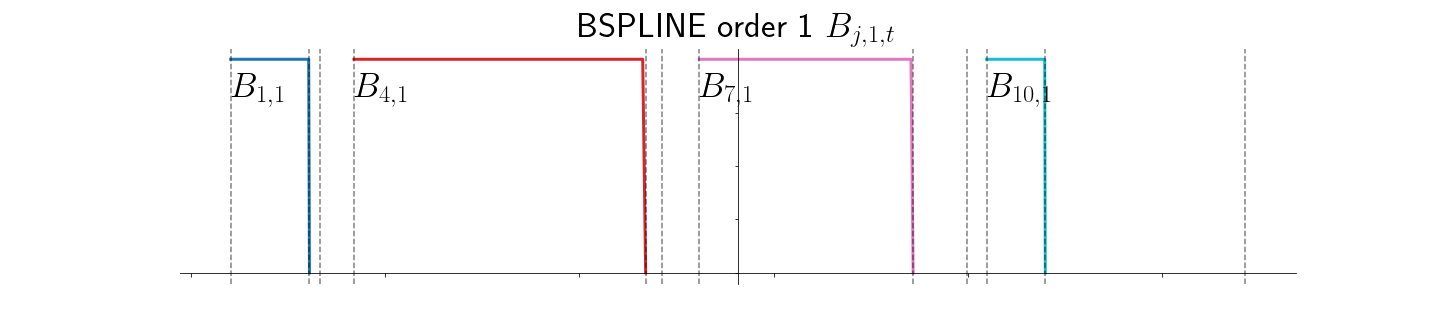
\includegraphics[width=\linewidth]{bspline_order_1.png}
	\caption{Some B-splines of order 1}\label{fig:bspline-order-1}
      \end{figure}
    \item \underline{$k=2$}
      \begin{align*}
        B_{j,2}(t) &= (t_{j+2}-t_j)\frac{[t_{j+1}, t_{j+2}]{(\cdot-t)}_+^1-[t_{j}, 
        t_{j+1}]{(\cdot-t)}_+^1}{t_{j+2}-t_j}\\
        &= \frac{{(t_{j+2}-t)}_+^1-{(t_{j+1}-t)}_+^1}{t_{j+2}-t_{j+1}}- 
        \frac{{(t_{j+1}-t)}_+^1-{(t_{j}-t)}_+^1}{t_{j+1}-t_{j}} \\
        &= 
        \begin{dcases}
	  \frac{t-t_j}{t_{j+1}-t_j} & t_j \leq t < t_{j+1},\\
	  \frac{t_{j+2}-t}{t_{j+2}-t_{j+1}} & t_{j+1} \leq t < t_{j+2}, \\
	0 & \mathrm{elsewhere}.
      \end{dcases}
      \end{align*}
      \begin{figure}[!h]
	\centering
	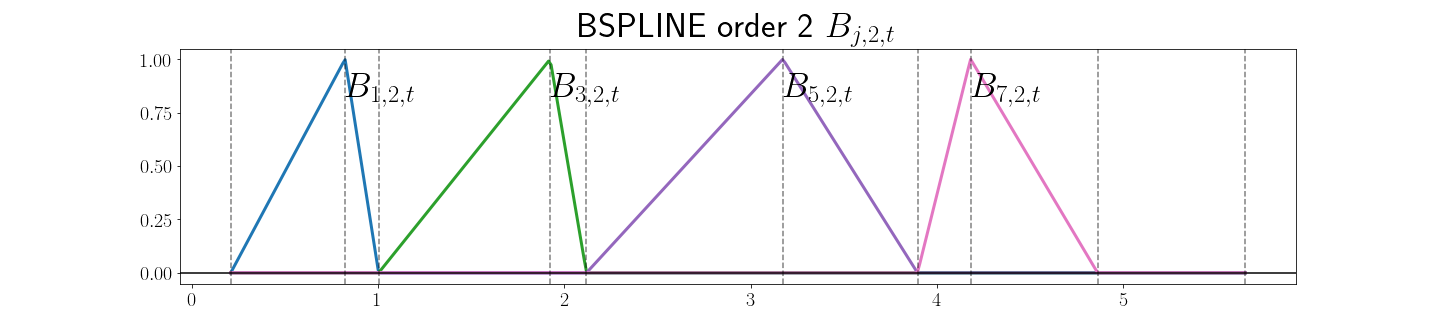
\includegraphics[width=\linewidth]{bspline_order_2.png}
	\caption{Some B-splines of order 2}\label{fig:bspline-order-2}
      \end{figure}
  \end{itemize}
\end{example}

\begin{remark}
  \begin{enumerate}
    \item Schoenberg also defined a general B-spline~\cite[Lecture 1, (2.1)]{schoenberg_cardinal_1973-1}) as
    \begin{equation*}
      M_{j,k,\bm{t}}(t) = k[t_j, \ldots, t_{j+k}]{(\cdot-t)}_+^{k-1}.
    \end{equation*}
    It is related to De Boor's general B-spline as
    \begin{equation*}
      \frac{k}{t_{j+k}-t_j}B_{j,k,\bm{t}},
    \end{equation*}
    which yields to the same definition provided that $t_{j+k} - t_j = k$.
  \item De Boor's \emph{B-splines} are the same as Schoenberg's forward B-splines (\ref{eq:fbspline})  when
    $\bm{t} = \mathbb{Z}$, i.e,
    \begin{equation*}
      B_{j,k,\mathbb{Z}}(t) = Q_k(t-j).
    \end{equation*}
  \end{enumerate}
\end{remark}

From the definition of B-splines in the most general case, a \emph{spline} is defined as follows
\begin{deftn}[{\cite[Chapter IX, (26)]{de_boor_practical_2001}}]\label{def:gen-splines}
  A spline function of order $k$ with knot sequence $\bm{t}$ is a linear combination of B-splines. $\mathscr{S}_{k, 
  \bm{t}}$ denotes the collection of all such splines, i.e,
  \begin{equation*}
    \mathscr{S}_{k, \bm{t}} := \{ \sum_{i=-\infty}^{\infty} c_i B_{i,k,\bm{t}} | \bm{c} \in \mathbb{R}^{\mathbb{Z}}\}
  \end{equation*}
\end{deftn}

\begin{remark}
  In the definition above, the sum is infinite while $\bm{t}$, and therefore the set $(B_{i, k,\bm{t}})$, may be finite 
  by assumption. When $\bm{t}$ is finite, choose $c_i=0$ for every $i$ where $B_{i,k,\bm{t}}$ is not defined. In the 
  properties given afterwards, we will voluntarily leave the limits of the sum unspecified. We could have restricted 
  ourselves to infinite sequences of knots $\bm{t}$, but it is an unnecessary limitation as all results hold for finite 
  sequences, albeit with different notations.
\end{remark}

As suggested in the subsection title, the approach used by De Boor mirrors that of Schoenberg.  Schoenberg first defines 
cardinal splines and then goes on to prove that cardinal B-splines form a basis for the collection formed by the 
cardinal splines. De Boor chooses to start by defining B-splines and later on defines splines as those functions that 
are written as linear combinations of B-splines. In the end, both definitions are equivalent, given 
Theorem~\ref{thm:curry-sch}, proposed by Curry and Schoenberg. Let us define the \textit{basic interval} $I_{k, \bm{t}}$  
as follows
\begin{equation*}
  I_{k, \bm{t}} = (t_-, t_+), \quad t_- := 
  \begin{dcases} t_k & \text{if} \ \bm{t} = (t_1, \ldots) \\ \inf t_j & \text{otherwise} \end{dcases}, 
  \quad t_+ := \begin{dcases} t_{n+1} & \text{if} \ \bm{t} = (\ldots, t_{n+k}) \\ \sup t_j & \text{otherwise} 
  \end{dcases}.
\end{equation*}
In the following proposition, we summarize the most useful properties of B-splines.
\begin{prop}[{\cite[Chapters IX, X, XI]{de_boor_practical_2001}}]
  \begin{enumerate}
    \item (Recurrence relation) \begin{equation*}
	B_{i,k} = \omega_{i,k} B_{i,k-1} + (1-\omega_{i+1,k})B_{i+1, k-1},
      \end{equation*}
      with
      \begin{equation*}
	\omega_{i,k}(t) = \frac{t-t_i}{t_{i+k-1}-t_i}.
      \end{equation*}
    \item (Marsden's identity)
      For any $\tau \in \mathbb{R}$, \begin{equation*}
	{(\cdot-\tau)}^{k-1} = \sum_{i} \psi_{i,k}(\tau) B_{i,k},
      \end{equation*}
      with 
      \begin{equation*}
	\psi_{i,k}(\tau) := (t_{i+1}-\tau)\cdots(t_{i+k-1}-\tau).
      \end{equation*}
    \item (Reproduction capabilities)
      From Marsden's identity,
      \begin{equation*}
	\Pi_{<k} \subset \mathscr{S}_{k, \bm{t}}.
      \end{equation*}
      In particular, $(B_{i,k})$ is a local partition of unity, i.e,
      \begin{equation*}
	\sum_{i} B_{i,k} = 1 \quad \mathrm{on} \ I_{k, \bm{t}}.
      \end{equation*}
    \item (Uniqueness and stability)
      There exists a positive constant $D_{k, \infty}$ independent of $\bm{t}$ such that
      \begin{equation*}
	\forall \bm{c} \in \mathbb{R}^{\mathbb{Z}}, \quad D_{k, \infty}^{-1} {\|\bm{c}\|}_{\infty} \leq {\left\| 
	\sum_{i} c_{i} B_{i,k} \right\|}_{\infty} \leq {\|\bm{c}\|}_{\infty}.
      \end{equation*}
  \end{enumerate}
\end{prop}
The spline space $\mathscr{S}_{k,\bm{t}}$ is finally completely characterized by the Curry-Schoenberg theorem, which 
also unveils its connection with piecewise-polynomial functions.
\begin{thm}[\cite{curry_polya_1966},{\cite[Chapter IX, (44)]{de_boor_practical_2001}}]\label{thm:curry-sch}
  Let $l \in \mathbb{N}^*$. For a given increasing sequence $\bm{\xi} = {(\xi_i)}_{i \in \llbracket1,l+1\rrbracket}$, 
  and a given nonnegative sequence of integers $\bm{\nu} = {(\nu_i)}_{i \in \llbracket2,l\rrbracket}$ with $\nu_i \leq  
  k$, set \begin{equation*}
    n := kl - \sum_{i=2}^{l} k - \nu_i = \dim \Pi_{<k, \bm{\xi}, \bm{\nu}}
  \end{equation*}
  and let $\bm{t} = {(t_i)}_{i \in \llbracket1,n+k\rrbracket}$ a nondecreasing sequence obtained from $\xi$ such that
  \begin{enumerate}
    \item for $i \in \llbracket2,l\rrbracket$, $\xi_i$ appears $k-\nu_i$ times in $\bm{t}$
    \item $t_1 \leq \ldots \leq t_k \leq \xi_1$ and $\xi_{l+1} \leq t_{n+1} \leq \ldots t_{n+k}$
  \end{enumerate}
  Then $B_{1,k}, \ldots, B_{n,k}$ is a basis for $\Pi_{k, \xi, \nu}$ on $I_{k,t} = [t_k,t_{n+1}]$, i.e,
  \begin{equation*}
    {\mathscr{S}_{k, \bm{t}}}_{|I_{k,t}} = {\Pi_{<k, \bm{\xi}. \bm{\nu}}}_{|I_{k,t}}.
  \end{equation*}
\end{thm}


% Include second chapter
\chapter{The Hermite interpolation problem}\label{chapter2}

From a historical perspective, the interpolation problem was intially stated as finding an interpolation function at 
equally-spaced locations, as described in Chapter~\ref{chapter1}. Later on, as the interest in interpolation grew among 
mathematicians, a number of more general formulas were indentified to cover fairly arbitrary point configurations.  
However, configurations with repeated interpolation point locations remained largely unexplored until the general 
problem formulated by Hermite in 1877~\cite{hermite_1877}. There, Hermite sets the task of finding a polynomial of 
degree $n-1$ that satisfies a total of $n$ interpolating conditions in the form of consecutive derivatives at distinct 
locations.  Theorem~\ref{thm:unique_pol} states that there exists a unique such polynomial, and we discussed how the 
interpolating polynomial can be written in \emph{Newton form}, using the extended divided difference operator. However,
the result does not extend to the problem of interpolating at an infinite number of locations, even when only values and 
not derivatives are to be reproduced, as the degree of the interpolating polynomial would then be infinite. Another 
approach to the problem, as previously mentioned at the end of Section~\ref{sec:splines}, is to break it down to an 
infinite number of finite interpolation problems. In that setting, the focus is restricted to a subset of the 
conditions, defining a \emph{piece} of the interpolant, before joining pieces in a smooth fashion.  This is the essence 
of splines, which are fundamental in our formulation of solutions to the so-called \emph{cardinal Hermite interpolation 
problem}.

\section{Schoenberg's theorems}

We here introduce the fundamental results of Schoenberg on the general problem of interpolating a function and a certain 
number of consecutive derivatives on the integer grid. Schoenberg dedicated a good part of his life to his work on 
splines, starting from his landmark paper~\cite{schoenberg_contributions_1946}, and continued with a series of papers 
among 
which~\cite{schoenberg_cardinal_1969},~\cite{schoenberg_cardinal_1972a},~\cite{schoenberg_cardinal_1972b},~\cite{lipow_cardinal_1973} 
and~\cite{schoenberg_cardinal_1973} are of particular relevance to our work. This section is highly inspired by his work 
to which we will refer a lot.  An elegant compilation Schoenberg's work on splines can be found 
in~\cite{schoenberg_cardinal_1973:1}, which contains 10 lectures, each presenting one specific aspect of splines while 
laying the foundations for the lectures that follows. We start by stating the notations that we will use throughout this 
chapter.

\begin{itemize}
  \itemsep0em
  \item $r, m, n \in \mathbb{N}^*$, $r \geq m$;
  \item $\mathbb{Z}_r = {\{ t_j=k | kr \leq j < k(r+1) \}}_{j \in \mathbb{Z}}$ is the set of integers repeated $r$ 
    times;
  \item $\mathscr{S}_{n}$ are the Schoenberg's cardinal splines of \emph{order} $n$    
    (Definition~\ref{def:card-splines});
  \item $\mathscr{S}_{n, \mathbb{Z}_r}$ are the De Boor's splines of order $n$ with knots on $\mathbb{Z}_r$ 
    (Definition~\ref{def:gen-splines});
  \item $\bm{y}^{(0)}, \ldots, \bm{y}^{(r-1)}$ are sequences of real numbers.
\end{itemize}

\subsection{The cardinal Hermite interpolation problem}

\begin{deftn}[C.H.I.P, {\cite[(10)-(12)]{lipow_cardinal_1973}}]
  The $r$ sequences of real numbers $\bm{y}^{(0)}, \ldots, \bm{y}^{(r-1)}$ being prescribed, the cardinal Hermite 
  interpolation problem (C.H.I.P) for the vector space $\mathcal{V}$, ($\bm{y}^{(0)}, \ldots, \bm{y}^{(r-1)}, 
  \mathcal{V}$), is the problem of finding a function $S \in \mathcal{V}$
  that agrees with the sequences $\bm{y}^{(0)}, \ldots, \bm{y}^{(r-1)}$ in the sense that
  \begin{equation}\label{def:chip}
    \forall \rho \in \llbracket0,r-1\rrbracket, \quad \forall k \in \mathbb{Z}, \quad S^{(\rho)}(k) = y^{(\rho)}_k
  \end{equation}
\end{deftn}
\noindent In non-mathematical words, a C.H.I.P aims at interpolating an unknown function for which we only have samples 
of its values and possibly its derivatives on a uniformly-spaced grid. Such questions arise in signal processing and 
image nalysis, where the uniform grid is the array detector of a camera and the samples are the pixels, all of which 
form an image. An image is thus only a discretized version of an underlying continuous reality that we would like to 
approximate from the pixels. One such continuous reality could, for instance, be the surface of a cell, which, when 
successfully modelled, can increase our understanding of its mechanical and biological properties.\\

In Chapter~\ref{chapter1}, the space of cardinal splines of order $n$, $\mathscr{S}_n$, was defined as those functions 
that are polynomials of order $n$ on all intervals $(k, k+1)$ for $k \in \mathbb{Z}$ and that belong to the class 
$\mathcal{C}^{n-2}$. It is possible and relevant for the Hermite interpolation problem to consider similar functions 
with less degrees of continuity at the joining points.
\begin{deftn}[{\cite[Lecture 5]{schoenberg_cardinal_1973-1}}]
  The set $\mathscr{S}_{n, r}$ of cardinal splines of \emph{order} $n$ and \emph{multiplicity} $r$ denotes all functions 
  $S$ such that
  \begin{enumerate}
    \item $S \in \Pi_{<n}$ on $(k, k+1)$ for $k \in \mathbb{Z}$;
    \item $S \in \mathcal{C}^{n-r-1}$.
  \end{enumerate}
  At times, it is convenient to consider the splines halfway between the integers, that is,
  \begin{equation*}
    \mathscr{S}^*_{n,r} = \{S | S(\cdot + \frac{1}{2}) \in \mathscr{S}_{n,r}\}.
  \end{equation*}
\end{deftn}

\begin{remark}
  This new set of splines connects to the sets defined in Definition~\ref{def:ppol-cont},~\ref{def:gen-splines}
  \begin{equation*}
    \mathscr{S}_{n,r} = \mathscr{S}_{n, \mathbb{Z}_r} = \Pi_{<n, \mathbb{Z}, \bm{\nu}},
  \end{equation*}
  where $\bm{\nu}$ is the constant sequence with value $n-r$. Also, splines of order $n$ for the particular case of 
  multiplicity $r=1$ are cardinal splines as in Definition~\ref{def:card-splines}, i.e,
  \begin{equation*}
    \mathscr{S}_n = \mathscr{S}_{n,1}.
  \end{equation*}
\end{remark}
\noindent Solutions for the C.H.I.P~\ref{def:chip} are readily obtained in the form of functions in $S_{n,r}$ or $S_{n, 
r}^*$ as expressed in the following lemma.
\begin{lem}\label{lemma:manifold}
  \begin{enumerate}
    \item The Hermite interpolation problem~\ref{def:chip} with $\mathcal{V}=\mathscr{S}_{n,r}$ has infinitely many 
      solutions that form a linear manifold of dimension $n-2r$.
    \item The Hermite interpolation problem~\ref{def:chip} with $\mathcal{V}=\mathscr{S}_{n,r}^*$ has infinitely many 
      solutions that form a linear manifold of dimension $n-r$.
  \end{enumerate}
\end{lem}

The proof is given in Appendix~\ref{chapter:annexA}, extending Schoenberg's proof of (\cite[Lemma 1.1, Lecture 
4]{schoenberg_cardinal_1973-1}) for cardinal interpolation, which is none other than cardinal Hermite interpolation for 
$r=1$. An immediate corollary of this lemma for the sequences to be interpolated that vanish identically is obtained as 
follows.

\begin{lem}\label{lemma:linear-space}
  Define 
  \begin{align}\label{def:ringsplines}
    \mathring{\mathscr{S}}_{n, r} &= \{S \in \mathscr{S}_{n,r}| S^{(\rho)}(k) = 0, \rho=0, \ldots, r-1, k \in 
    \mathbb{Z}\}; \\
    \mathring{\mathscr{S}}_{n,r}^* &= \{S \in \mathscr{S}_{n,r}^*| S^{(\rho)}(k) = 0, \rho=0, \ldots, r-1, k \in 
    \mathbb{Z}\}.
  \end{align}
  Then, $\mathring{\mathscr{S}}_{n, r},  \mathring{\mathscr{S}}_{n, r}^*$ are linear spaces with
  \begin{equation}
    \dim \mathring{\mathscr{S}}_{n,r} = n-2r, \quad \dim \mathring{\mathscr{S}}_{n,r}^* = n-r.
  \end{equation}
\end{lem}

\begin{proof}
  The proof is immediate using Lemma~\ref{lemma:manifold}. Indeed, $\mathring{\mathscr{S}}_{n,r}$ is exactly the set of 
  solutions to the C.H.I.P ($0, \ldots, 0, \mathscr{S}_{n,r}$), which is not only a linear manifold but also a linear 
  space as it contains the trivial spline. Furthermore, it has dimension $n-2r$. A similar reasoning applies to 
  $\mathring{\mathscr{S}}_{n,r}^*$.
\end{proof}

\subsection{Spline interpolant to sequences of power growth}

Let $\gamma \geq 0$ be a nonnegative real number and let
\begin{align}
  \mathcal{Y}^{\gamma} &= \{\bm{y} \in \mathbb{R}^{\mathbb{Z}} | y_k = \mathcal{O}_{|k| \to \infty}({|k|}^{\gamma})\},\\
  \mathscr{S}_{n, r}^{\gamma} &= \{S \in \mathscr{S}_{n,r} | S(t) = \mathcal{O}_{|t| \to \infty}({|t|}^{\gamma})\},
\end{align}
be respectively the spaces of power growth sequences and power growth splines with power $\gamma$.  As mentioned by in 
after (\cite[(2.1)]{schoenberg_cardinal_1973-1}), application of Markov's theorem on bounds shows that all derivatives 
of $S \in \mathscr{S}_{n,r}^{\gamma}$ satisfy the same decay condition. This is something Schoenberg most probably 
noticed after publishing (\cite{lipow_cardinal_1973}) as, in the latter, he defines $\mathscr{S}_{n, r}^{\gamma}$ as the set of splines 
whose derivatives up to $r-1$ are of power growth $\gamma$. \\

From now on we assume that $n=2m$ is an even number with $m \geq r$. This is the choice made by Lipow and Schoenberg n 
(\cite{lipow_cardinal_1973}) in order to avoid rewriting known results with slightly different notations.  Indeed, all 
results for even values of $n$ are easily extended to the case of odd values of $n$ using the spline space $S_{n,r}^*$ 
and all subsequently defined sets as we did in Lemma~\ref{lemma:manifold}.  This lemma also shows that the 
C.H.I.P~\ref{def:chip} has an infinite number of solutions in the form of splines. However, if we consider functions in 
the set $\mathscr{S}_{2m,r}^{\gamma}$ of splines with power growth $\gamma$, the set of solutions to ($\bm{y^{(0)}}, 
\ldots, \bm{y^{(r-1)}}, \mathscr{S}_{2m,r}^{\gamma}$) reduces to a unique element provided that the sequences satisfy 
the same power growth. This is the topic of the following theorem, which is the main result and is central to the theory 
of Hermite interpolation

\begin{thm}[{\cite[Theorems 1,4]{lipow_cardinal_1973}}]\label{thm:LH-gamma}
  The C.H.I.P ($\bm{y}^{(0)}, \ldots, \bm{y}^{(r-1)}, \mathscr{S}_{2m,r}^{\gamma})$ has a unique solution if and only if 
  $\bm{y}^{(0)}, \ldots, \bm{y}^{(r-1)}$ are in  $\mathcal{Y}^{\gamma}$. In that case, the solution is explicitly given 
  by the Lagrange-Hermite expansion
  \begin{equation}\label{eq:LH}
    S(t) = \sum_{k=-\infty}^{\infty} \sum_{s=0}^{r-1} y_k^{(s)} L_s(t-k)
  \end{equation}
  where $L_0, \ldots, L_{r-1}$ are the fundamental splines as defined in Definition~\ref{def:fundamental-r}. This 
  expansion converges absolutely and locally uniformly.
\end{thm}
\noindent The full proof is provided in~\cite{lipow_cardinal_1973} and~\cite[Lecture 5]{schoenberg_cardinal_1973-1}. We 
hereafter give a sketch of the proof and refer the reader to~\cite{lipow_cardinal_1973} for details. 
  
\begin{proof}[Proof sketch]
  \textbf{(Unicity)} We start by noticing that the difference of two solutions $S$ belongs to 
  $\mathring{\mathscr{S}}_{2m, r}^{\gamma}$.  From Lemma~\ref{lemma:linear-space}, this set is a linear space of 
  dimension $2m-2r$. The $2m-2r$ ``eigensplines'' $\{S_1, \ldots, S_{2m-2r}\}$ (Definition~\ref{def:eigsplines-r}) form 
  a basis of this linear space (\cite[Lemma 3, Lecture 5]{schoenberg_cardinal_1973-1}). As a consequence, there exist 
  coefficients $c_1, \ldots, c_{2m-2r}$ such that
  \begin{equation}\label{eq:diff-expansion}
    S = \sum_{j=1}^{2m-2r} c_j S_{j}.
  \end{equation}
  Eigensplines behaving towards infinity as~\cite[(5.16), (5.17)]{lipow_cardinal_1973}
  \begin{align}
    0 &< \overline{\lim}_{x \to -\infty} \frac{|S_{j}(x)|}{|\lambda_{j}|^x} < \infty \quad j=1, \ldots, m-r, \\
    0 &< \overline{\lim}_{x \to \infty} \frac{|S_{j}(x)|}{|\lambda_{j}|^x} < \infty \quad j=m-r+1, \ldots, 2m-2r,
  \end{align}
  and $S(t) = \mathcal{O}_{|t|\to\infty}(|t|^{\gamma})$ having power growth $\gamma$ at infinity, all the coefficients 
  must vanish and so does $S$.  \\

  \textbf{(Existence)} An explicit solution is constructed using an expansion in terms of \emph{fundamental} splines 
  ${L_s := L_{2m,r,s}}$ for $s \in \llbracket0,r-1\rrbracket$ (Definition~\ref{def:fundamental-r}). They are defined as 
  bounded functions such that $L_s$ and $s$ have the same parity and
  \begin{equation*}
    L_s(t) = \begin{dcases} P_s(t) & \text{if} \ 0 \leq t \leq 1, \\
    \sum_{j=1}^{m-r} c_{j,s} S_j(t) & \text{if} \ t \geq 1, \end{dcases}
  \end{equation*}
  with
  \begin{equation*}\scriptstyle
    P_s(t) = \begin{dcases}\scriptstyle \frac{1}{s!}t^s + a_{1,s}t^r + a_{2,s}t^{r+2} + \cdots + a_{m-r+1,s}t^{2m-r} + 
      a_{m-r+2,s} t^{2m-r+1} + \cdots + a_{m,s} t^{2m-r} & \text{if $2|(r-s)$} \\
      \scriptstyle\frac{1}{s!}t^s + a_{1,s}t^{r+1} + a_{2,s}t^{r+3} + \cdots + a_{m-r,s}t^{2m-r-1} + a_{m-r+1,s} 
      t^{2m-r} + \cdots + a_{m,s} t^{2m-r} & \text{otherwise},
   \end{dcases}
  \end{equation*}
  where the $2m-r$ unknowns $a_{1,s}, \ldots, a_{m,s}, c_{1,s}, \ldots, c_{m-r,s}$ defining $L_s$ are obtained as the 
  unique solution of the linear system of $2m-r$ equations
  \begin{equation*}
    \forall \rho \in \llbracket0,2m-r-1\rrbracket, \qquad P_s^{(\rho)}(1) =\sum_{j=1}^{m-r} c_{j,s} S_j^{(\rho)}(1).
  \end{equation*}
  The solution is unique because the associated homogeneous system (removing the $\frac{1}{s!}t^s$) is non-singular.  
  Indeed, if it were to be singular, there would exist a non trivial bounded spline in $\mathscr{S}_{2m,r}^{0}$
  that vanishes with all its derivatives up to order $r-1$. However, from the proof of unicity we know that there can be 
  at most one such spline. The trivial spline being one of of them leads to a contradiction.\\

  A solution to the C.H.I.P ($\bm{y}^{(0)}, \ldots, \bm{y}^{(r-1)}, \mathscr{S}_{2m,r}^{\gamma})$ is then given by
  \begin{equation*}
    S(t) = \sum_{k=-\infty}^{\infty} \sum_{s=0}^{r-1} y_k^{(s)} L_s(t-k),
  \end{equation*}
  since, by construction, the \emph{fundamental} splines $L_s$ are in $\mathscr{S}_{2m,r}^0 \subset 
  \mathscr{S}_{2m,r}^{\gamma}$ and satisfy
  \begin{equation}\label{eq:fund-prop}
    \forall \rho \in \llbracket0,r-1\rrbracket, \qquad \forall k \in \mathbb{Z}, \quad L_s^{(\rho)}(k) = 
    \delta_{k}\delta_{s-\rho}.
  \end{equation}
  This completes the proof.
\end{proof}

These results have been extended to the cases of sequences in $l^p$ for $1 \leq p \leq \infty$, where the interpolating 
spline is a function in the set 
\begin{equation*}
  \mathcal{L}^p_r = \{F:\mathbb{R} \to \mathbb{C}| F^{(\rho)} \in \mathcal{L}^p(\mathbb{R}, \mathbb{C}), \rho=0, \ldots, 
  r-1\}.
\end{equation*}

\begin{thm}[{\cite[Theorems 2,4]{lipow_cardinal_1973}}]\label{thm:LH-p} Let $1 \leq p \leq \infty$. The C.H.I.P 
  ($\bm{y}^{(0)}, \ldots, \bm{y}^{(r-1)}, \mathscr{S}_{2m,r}\cap L^p_r)$ has a unique solution if and only if 
  $\bm{y}^{(0)}, \ldots, \bm{y}^{(r-1)}$ are in  $l^p$. In that case, the solution is explicitly given by the 
  Lagrange-Hermite expansion
  \begin{equation}
    S(t) = \sum_{k=-\infty}^{\infty} \sum_{s=0}^{r-1} y_k^{(s)} L_s(t-k).
  \end{equation}
  This expansion converges absolutely and locally uniformly.
\end{thm}

\section{Hermite B-splines}

We refer to as \emph{generators} functions that span a given linear space in the usual algebraic sense.  This set of 
functions can be infinite as we shall see. In some cases, it is itself generated as all integer translates of a finite 
set of functions, to which we shall also refer to as \emph{generators} by extension. In that sense, the set of functions 
arising from the Whittaker-Shannon interpolation formula, expressed as
\begin{equation*}
  SW = \{y(t) = \sum_{k=-\infty}^{\infty} y_k \sinc(t-k) | y_k \in \mathcal{Y}\}
\end{equation*}
with $\mathcal{Y}$ all real or complex sequences satisfying $\displaystyle\sum_{k=-\infty, k\neq0}^{\infty} 
|\frac{y_k}{k}|<\infty$ is generated by the infinite set of functions ${\{\sinc(\cdot-k)\}}_{k \in \mathbb{Z}}$. This 
infinite set of functions is itself generated by integer translates of the single function $\{\sinc\}$. We shall thus 
refer to $\sinc$ as a generator for the space $SW$. In that sense also, the $r$ fundamental splines $\{L_0, \ldots, 
L_{r-1}\}$ are generators for the linear space
\begin{equation}\label{eq:def-V}
  V = \{S(t) = \sum_{k=-\infty}^{\infty} \sum_{s=0}^{r-1} c_{k,s} L_s(t-k) | c_0, \ldots, c_{r-1} \in 
\mathbb{R}^{\mathbb{Z}}\}
\end{equation}
The functions appearing as infinite sums in (\ref{eq:def-V}) may not always be properly defined, in which case
conditions must be set on sequences for the series to converge. From Theorem~\ref{thm:LH-gamma} and 
Theorem~\ref{thm:LH-p}, we know that, if the sequences of coefficients are in $\mathcal{Y}^{\gamma}$ or in $l^p$, then 
the series converges locally uniformly to a function in $S_{2m, r}^{\gamma}$ or $S_{2m, r}\cap L^p_r$ respectively. \\

Many questions naturally arise about the properties of the generators and the properties of the generated functions. The 
next section introduces the Hermite B-splines, closely related to $L_{2m,r,0}, \ldots, L_{2m, r, r-1}$, while an 
extensive study of their properties is postponed until Chapter~\ref{chapter3}.

\subsection{Definition from fundamental splines}

The Hermite B-splines were first introduced in an attempt to extend the B-spline representation existing in the set 
$\mathscr{S}_n$ of splines of order $n$ to the set $\mathscr{S}_{n,r}$ of splines of order $n$ and multiplicity $r$.   
As was the case in the previous section, we continue to only consider even values of $n$ with $n=2m$.

\begin{deftn}[Hermite B-splines,{~\cite[Definition 1]{schoenberg_cardinal_1973}}]\label{def:hbsplines}
  The Hermite B-splines are the $r$ elements $N_{2m,r,0}, \ldots, N_{2m,r,r-1}$ of $\mathscr{S}_{2m,r}$ defined by 
  \begin{equation}\label{eq:def-hbsplines}
    N_{2m,r,s}(t) = \sum_{k=-(m-r)}^{m-r} c_k L_{2m,r,s}(t-k),
  \end{equation}
  with $c_k$ the coefficients of the Euler-Frobenius polynomial of multiplicity $r$ (Definition~\ref{def:EF-r}).
\end{deftn}

\begin{example}\label{ex:N0}
  Consider the case of multiplicity 1, \textit{i.e} $r=1$, in order to see how Hermite B-splines relate to $M_{2m}$, 
  B-splines of $S_{2m}$. As $M_{2m}$ is supported in $(-m,m)$, the sequence ${\bm{y} = {(M_{2m}(k))}_{k \in 
  \mathbb{Z}}}$ has at most $2m-1$ non zero elements and is hence bounded. From Theorem~\ref{thm:LH-gamma}, the 
  Lagrange-Hermite expansion for the bounded sequence $\bm{y}$ defines the unique bounded element in $\mathscr{S}_{2m,1} 
  = \mathscr{S}_{2m}$ that interpolates $\bm{y}$.  As $M_{2m}$ itself is one such element, unicity implies that this 
  Lagrange-Hermite expansion equals $M_{2m}$ everywhere, meaning that \begin{equation}\label{eq:expansion-M2m}
    \forall t \in \mathbb{R}, \qquad M_{2m}(t) = \sum_{k=-(m-1)}^{m-1} M_{2m}(k) L_0(t-k).
  \end{equation}
  From Definition~\ref{def:EF} of the Euler-Frobenius polynomial, we have that
  \begin{equation*}
    \Pi_{2m}(t) = (2m-1)! \sum_{k=-(m-1)}^{m-1} Q_{2m}(k+m) t^{k+m-1}.
  \end{equation*}
  However, from (\ref{eq:def-EF-r}), $(2m-1)!Q_{2m}(k+m)=c_k$. From (\ref{eq:cbspline}), ${Q_{2m}(k+m) = M_{2m}(k)}$.  
  Consequently, multiplying (\ref{eq:expansion-M2m}) by $(2m-1)! $ and replacing $(2m-1)!M_{2m}(k)$ by $c_k$ leads to
  \begin{equation*}
    \forall t \in \mathbb{R}, \quad (2m-1)!M_{2m}(t) = N_{2m,1,0}(t).
  \end{equation*}
\end{example}
The central B-spline $M_{2m}$ of order $2m$ is localized in the sense that it is supported within the compact set 
$[-m,m]$. Therefore, so is $N_{2m,1,0}$. The following lemma extends this observation to all Hermite B-splines of 
general multiplicity $r$.

\begin{lem}[{\cite[Lemma 2]{schoenberg_cardinal_1973}}]\label{lemma:supp-hbsplines}
  The Hermite B-splines $N_{2m,r,0}, \ldots, N_{2m,r,r-1}$ have their support in
  \begin{equation*}
    [-(m-r+1), m-r+1].
  \end{equation*}
  Moreover, for $s \in \llbracket0,r-1\rrbracket$, $N_{2m,r,s}$ has the same parity as $s$.
\end{lem}
The proof can be found in~\cite{schoenberg_cardinal_1973} and is reproduced in~\ref{proof:supp-hbsplines}. 

\subsection{Hermite B-splines form a basis}

The ``B'' in B-splines stands for basis. Therefore, the names of $N_{2m,r,0}, \ldots, N_{2m,r,r-1}$ suggest that they 
form a basis of some spline spaces together with their integer translates. This result is true, and we shall prove that, 
for $s \in \llbracket0,r-1\rrbracket$, $N_{2m,r,s}$ and its translates form a basis for the subspace
\begin{equation}\label{def:subspace-s}
  \mathscr{S}_{2m,r}^{(s)} = \{ S \in \mathscr{S}_{2m,r} | S^{(\rho)}(k) = 0, \rho \in \{0, \ldots, r-1\}\setminus 
  \{s\}, k \in \mathbb{Z}\}.
\end{equation}
Let $s \in \llbracket0,r-1\rrbracket$. Observe first that $N_{2m,r,s} \in \mathscr{S}_{2m,r}^{(s)}$. Indeed, combining 
(\ref{eq:fund-prop}) and (\ref{eq:def-hbsplines}) shows that
\begin{equation*}
  \forall \rho \in \llbracket0,r-1\rrbracket, \forall k \in \mathbb{Z}, \qquad N_s^{(\rho)}(k) = \delta_{s-\rho} 
  \sum_{l=-(m-r)}^{m-r} c_k \delta_{l-k}.
\end{equation*}
Thus, only derivatives of order $s$ of $N_{2m,r,s}$ may be non-zero on the integer grid. The definition 
(\ref{def:subspace-s}) indicates that $\mathscr{S}_{2m,r}^{(s)}$ is invariant by integer shift. Therefore, all integer 
translates of $N_{2m,r,s}$ are also in that subspace. The set $\mathscr{S}_{2m,r}^{(s)}$ being a linear space, any 
function $S$ of the form
\begin{equation}\label{eq:lc-hbsplines}
  S = \sum_{k=-\infty}^{\infty} c_{k} N_s(\cdot-k)
\end{equation}
is also in $\mathscr{S}_{2m,r}^{(s)}$, so that
\begin{equation*}
  \Span \{N_s(\cdot-k) | k \in \mathbb{Z} \} \subseteq \mathscr{S}_{2m,r}^{(s)}.
\end{equation*}
The function given by (\ref{eq:lc-hbsplines}) is well-defined for any sequence of coefficients since, at any real $t$,
the value $N_{2m,r,s}(t-k)$ does not vanish only for a finite number of integers $k$.  \\

It remains to be shown that any spline $S \in \mathscr{S}_{2m,r}^{(s)}$ can also be written as (\ref{eq:lc-hbsplines}) 
for a unique sequence $\bm{c}$. If that is the case, then $\{N_{2m,r,s}(\cdot-k) | k \in \mathbb{Z}\}$ is a basis for 
$\mathscr{S}_{2m,r}^{(s)}$ and the names ``Hermite B-splines'' is justified. In order to be able to prove that, 
Schoenberg and Sharma assume that the polynomial $\Pi_{2m,r}$ is irreducible over the rational field~\cite[Assumption 
1]{schoenberg_cardinal_1973}. This assumption is most probably true but is too complex compared to the arguments used so 
far and is therefore slightly unsatisfying. From there, one can then show that $\{N_{2m,r,s}(\cdot-k) | k \in 
\mathbb{Z}\}$ are locally linearly independent, meaning that that the relation 
\begin{equation*}
  \sum_{k=-(2m-2r+1)}^{0} c_k N_s(t-k) = 0, \quad  -(m-r+1) \leq t \leq -(m-r) 
\end{equation*}
can only hold if all the coefficients vanish as
\begin{equation*}
  c_{-(2m-2r+1)} = \cdots = c_0 = 0
\end{equation*}
It was however show~\cite{lee_b-splines_1975} that this assumption is not needed and the local linear independence always holds.
\begin{lem}[{\cite[Lemma 1]{lee_b-splines_1975}}]\label{lemma:lee73}
  For every $s \in \llbracket0, r-1\rrbracket$, the $2m-2r+2$ polynomials
  \begin{equation*}
    N_{2m,r,s}, N_{2m,r,s}(\cdot+1), \ldots, N_{2m,r,s}(\cdot+2m-2r+1)
  \end{equation*}
  are linearly independent over $\left(-(m-r+1), -(m-r)\right)$.
\end{lem}

The proof consists in establishing that the determinant of the matrix of an homogeneous system of equations is non-zero, 
which is quite technical. We refer to~\cite{lee_b-splines_1975} for details. \\

The following theorem can now be established and concludes our discussion.
\begin{thm}[{\cite[Theorem 3]{schoenberg_cardinal_1973}}]
  Every $S \in \mathscr{S}_{2m,r}^{(s)}$ admits a unique representation of the form
  \begin{equation}\label{eq:expansion-Ns}
    S = \sum_{k=-\infty}^{\infty} a_k N_{2m,r,s}(\cdot-k).
  \end{equation}
\end{thm}

\begin{proof} For $s\in \llbracket0,r-1\rrbracket$, let $N_s := N_{2m,r,s}$.
  \begin{enumerate}
    \item Let $S_0 \in \mathscr{S}_{2m,r}^{(s)}$ be such that $S_0(t) = 0$ for $t < 0$. Let $R_s$ be the forward Hermite 
      B-spline, \textit{i.e}, $R_s(t) = N_s(t-(m-r+1))$, so that $R_s$ is supported in $(0, 2m-2r+2)$. Let $a_0 = 
      \frac{S^{(s)}(1)}{R_s^{(s)}(1)}$. Consider the function
      \begin{equation*}
	S_1 = S_0 - a_0 R_s.
      \end{equation*}
      By construction, the function $S_1$ is in $\mathscr{S}_{2m,r}^{(s)} \subset \mathcal{C}^{2m-r-1}$ and vanish 
      identically on $(-\infty, 0)$.  Expanding it about 0 in its Taylor series shows that the order $2m$ polynomial 
      ${S_1}_{|(0,1)}$ can be written as
      \begin{equation*}
	S_1(t) = \sum_{k=2m-r}^{2m-1} \alpha_{k} t^k, \quad 0 < t < 1
      \end{equation*}
      From the definition (\ref{def:subspace-s}) of $\mathscr{S}_{2m,r}^{(s)}$, $S_1^{(\rho)}(1) = 0$ for $\rho=0, 
      \ldots, r-1, \rho \neq s$ but also $S_1^{(s)}(1) = 0$ by construction of $S_1$. These $r$ vanishing derivatives at 
      $1$ can only hold if the coefficients $\alpha_{k}$ vanish altogether, that is, $S_1$ vanishes on $(0,1)$.  
      Considering $a_1 = \frac{S_1^{(s)}(2)}{R_s^{(s)}(1)}$, and the function
      \begin{equation*}
	S_2 = S_1 - a_1 R_s(\cdot-1),
      \end{equation*}
      we see that $S_2$ vanishes on $(1,2)$ and by extension and $(-\infty, 2)$. Continuing in like manner, we have
      \begin{equation*}
	S_0 = \sum_{k=0}^{\infty} a_k R_s(\cdot-k),
      \end{equation*}
      with the coefficients ${(a_k)}_{k \geq 0}$ uniquely determined. \\
    \item Let $S \in \mathscr{S}_{2m,r}^{(s)}$. As 
      \begin{equation*}
	R_s(t), \ldots, R_s(t+2m-2r+1), \qquad 0 \leq t \leq 1,
      \end{equation*}
      are linearly independent on $(0,1)$ (Lemma~\ref{lemma:lee73}), there exist unique coefficients $a_{-2m+2r-1}, 
      \ldots, a_0$ such that
      \begin{equation*}
	S(t) = \sum_{k=-(2m-2r+1)}^{0} a_k R_s(t-k), \qquad 0 < t < 1,
      \end{equation*}
      Indeed, $S_{|(0,1)}$ is a polynomial of order $2m$ satisfying 
      \begin{equation*}
	S^{(\rho)}(0) = S^{(\rho)}(1) = 0, \qquad \rho=0, \ldots, r-1, \rho \neq s.
      \end{equation*}
      This make a total of $2r-2$ constraints. As a consequence, the set of all polynomial or order $2m$ satisfying 
      these constraints is a linear space of dimension $2m-2r+2$. As the $2m-2r+2$ B-splines $R_s$ are linearly 
      independent and satisfy the constraints, they span that linear space. \\ 

      Now, the function
      \begin{equation*}
	S_0(t) = S(t) - \sum_{k=-(2m-2r+1)}^{0} a_k R_s(t-k)
      \end{equation*}
      vanishes on $[0,1]$. Let,
      \begin{equation*}
	S_1(t) = \begin{dcases} S_0(t) &  \text{if} \ t \geq 1 \\
	  0 & \text{otherwise}
	\end{dcases},
	\quad
	S_2(t) = \begin{dcases} S_0(t) &  \text{if} \ t \leq 0 \\
	  0 & \text{otherwise}
	\end{dcases}.
      \end{equation*}
      Applying the first case shows that 
      \begin{equation*}
	S_1(t) = \sum_{k=1}^{\infty} a_k R_s(t-k), \quad S_2(t) = \sum_{k=-\infty}^{-(2m-2r+2)} a_k R_s(t-k)
      \end{equation*}
      for unique coefficients ${(a_k)}_k$. Putting all pieces together, and defining $b_k = a_{k-(m-r+1)}$ we have that
      \begin{equation*}
	\forall t \in \mathbb{R}, \quad S(t) = \sum_{k=-\infty}^{\infty} b_k N_s(t-k).
      \end{equation*}
  \end{enumerate}
\end{proof}

\section{Applications to bio-image analysis}

The past decade saw a multiplication in the number of images recorded and in the number of acquisition techniques.  As a 
consequence, the need for automatic image analysis tools grew significantly in many research communities. More 
precisely, shape-modelling is of particular interest for many purposes, going from image segmentation to interactive 
modelling of curves and surfaces. In all applications of shape-modelling there is a need for intuitive user interaction, 
which is best achieved when the representation is interpolatory. Domains related to interactive curves or shape modelling 
include computer graphics, biomedical imaging, industrial design, modelling of animated surfaces, etc.  Shape-modelling 
techniques can be categorized between discrete and continuous methods.  Discrete methods include polygonal meshes and 
subdivision schemes, which allow to locally refine shapes, but are poorly suited for theoretical modelling.  
Continuous-domain methods in contrast offer good theoretical properties. They usually consist of Bézier shapes or 
splines-based models. The most used splines-based method is the NURBS model, but it generally cannot be smooth and 
interpolatory at the same time. We refer to as \emph{active contour} a computational tool for detecting and outlining 
objects in digital images.  We hereafter present splines-based active contours models, with applications to biomedical 
imaging or computer graphics, that are practically convenient and theoretically powerful. \\

In an ideal setting, the basis functions generating the active contour are smooth, compactly supported, interpolatory 
and allow to vary the resolution of the constructed shape.  

\subsection{Modelling of 2D contours}\label{ssec:2d}

\subsubsection{Hermite polynomial}

In 2016, V.Uhlmann et al\@. published a paper~\cite{uhlmann_hermite_2016} that presents practical use-cases and good 
practical properties of the Hermite fundamental splines $L_0 := L_{4,2,0}$ and $L_1 := L_{4,2,1}$ for active contour 
modelling.  More precisely, if $r[0], \ldots, r[M-1]$, $r'[0], \ldots, r'[M-1]$ are $M$ measurements of the value and 
first derivative value of a M-periodic closed 2D curve, a good interpolatory model for the curve is the Lagrange-Hermite 
expansion~\ref{eq:LH}, that is,
\begin{align*}
  \forall t \in \mathbb{R}, \qquad r(t) &= \sum_{k=-\infty}^{\infty} r[k] L_0(t-k) + r'[k] L_1(t-k) \\
  &= \sum_{k=0}^{M-1} r[k] L_{0,per}(t-k) + r'[k] L_{1,per}(t-k) \end{align*}
with $L_{0,per}, L_{1,per}$ the M-periodizations of the functions $L_0, L_1$ respectively.  

\begin{remark}
  \begin{enumerate}
    \item In contrast to the expansion~\ref{eq:LH}, the terms in front of the fundamental splines are not scalars but 2D 
      vectors. The formula above is in fact short for the interpolation of each coordinate separately $(r_1(t), r_2(t)) 
      = r(t)$, \textit{i.e},
      \begin{align*}
	\forall t \in \mathbb{R}, \qquad r_1(t) &= \sum_{k=0}^{M-1} r_1[k] L_{0, per}(t-k) + r_1'[k] L_{1,per}(t-k) \\
	\qquad r_2(t) &= \sum_{k=0}^{M-1} r_2[k] L_{0,per}(t-k) + r_2'[k] L_{1,per}(t-k)
      \end{align*}
    \item In the vocabulary of active contour modelling, the $(r[k],r'[k])_{k \in \llbracket0,M-1\rrbracket}$ are called 
      the \emph{control points} at the \emph{knots} $(k)_{k \in \llbracket0,M-1\rrbracket}$ respectively.
    \item The set of all functions that are can be written as linear combinations of ${\{L_{4,2,0}(\cdot-k), 
      L_{4,2,1}(\cdot-k)\}}_{k \in \mathbb{Z}}$ are called \emph{cubic Hermite splines}.
  \end{enumerate}
\end{remark}

The functions $L_0$ and $L_1$ are explicitly given by
\begin{equation}
    L_0(t) = \begin{dcases}
      1-3|t|^2 + 2|t|^3 &\text{for } 0 \leq |t| \leq 1,\\
      0 &\text{for } 1 < |t|,\\
    \end{dcases} \quad
    \hfill
    L_1(t) = \begin{dcases}
      t(|t|^2-2|t|+1) &\text{for } 0 \leq |t| \leq 1,\\
      0 &\text{for } 1 < |t|.\\
    \end{dcases}
\end{equation}
The graphs of these functions are displayed in Figure~\ref{fig:fund-r2-m2}. They are by definition Hermite splines of 
order 4 and multiplicity $2$. On top of that, the functions $L_0$, $L_1$ are: compactly supported with support of size 
2; $\mathcal{C}^1$ continuous; interpolatory with multiplicity 2 (value and derivative value) at integers; capable of 
reproducing cubic and quadratic splines; a partition of unity; a Riesz basis with Riesz bounds $A, B = 
(210^{\frac{-1}{2}}, B)$~\cite{uhlmann_hermite_2016}.

\subsubsection{Hermite exponential}

In 2015, Conti et al\@. presented in~\cite{conti_ellipse-preserving_2015} practical uses of a non-polynomial Hermite 
active contour model. The study in the paper was motivated by the observation that usual spline-based deformable models  
were unable to reproduce shapes as elementary as ellipses. More precisely, a lot of control points are needed to 
satisfyingly approximate ellipses. In contrast, in~\cite{conti_ellipse-preserving_2015}, authors devised a new Hermite 
interpolation scheme that perfectly reproduce ellipses but also retain attractive properties of cubic Hermite splines.  
\\

Let $\varphi_1, \varphi_2$ be the new basis functions. In order to have a Hermite interpolatory scheme, it is enough to 
choose the basis functions $\varphi_1, \varphi_2$ so that
\begin{equation*}
  \forall k \in \mathbb{Z}, \forall \rho \in \{0,1\}, \qquad \varphi_1^{(\rho)}(k) = \delta_{\rho}\delta_k, \quad 
  \varphi_2^{(\rho)}(k) = \delta_{\rho-1}\delta_k.
\end{equation*}

In order to reproduce ellipses from $M$ control points, the space spanned by ${\{\varphi_0(\cdot-k), 
\varphi_1(\cdot-k)\}_{k \in \mathbb{Z}}}$ should include the cosinus and sinus functions at frequency $\frac{1}{M}$, 
\textit{i.e},
\begin{align*}
  \cos (wt) &= \sum_{k=-\infty}^{\infty} \cos (wk) \varphi_1(t-k) - w \sin (wk) \varphi_2(t-k), \\
  \sin (wt) &= \sum_{k=-\infty}^{\infty} \sin (wk) \varphi_1(t-k) + w \cos (wk) \varphi_2(t-k),
\end{align*}
with $w = \frac{2\pi}{M}$.

The following functions were found to satisfy all the requirements,
\begin{align*}
  \varphi_{1, w}(x) &=
  \begin{dcases}
    g_{1,w} = a_1(w) + b_1(w)x + c_1(w) e^{jwx} + d_1(w)e^{-jwx} &\text{for } x \geq 0 \\
    g_{1, w}(-x) &\text{for } x < 0\\
  \end{dcases}, \\
  \varphi_{2, w}(x) &=
  \begin{dcases}
    g_{2, w}(x) =  a_2(w) + b_2(w)x + c_2(w) e^{jwx} + d_2(w)e^{-jwx} &\text{for } x \geq 0 \\
    -g_{2, w}(-x) &\text{for } x < 0\\
  \end{dcases},
\end{align*}
with $a_1(w), \ldots, d_1(w), a_2(w), \ldots, d_2(w)$ as in~\cite[(2), (3), (4)]{conti_ellipse-preserving_2015}.

The graphs of these functions are displayed in Figure~\ref{fig:conti_phi_12}.
\begin{figure}[!h]
  \centering
  \includegraphics[width=\textwidth]{conti_phi_12.png}
  \caption{Graphs of $\varphi_{1,w}, \varphi_{2,w}$ for $w=\frac{2\pi}{3}$}\label{fig:conti_phi_12}
\end{figure}

The functions $\varphi_1, \varphi_2$ are exponential splines (Definition~\ref{def:exponential-spline}). On top of that, 
the functions $\varphi_1$, $\varphi_2$ are: compactly supported with support of size 2; $\mathcal{C}^1$ continuous; 
interpolatory with multiplicity 2 (value and derivative value) at integers; capable of reproducing cubic and quadratic 
exponential splines; a partition of unity; a Riesz basis~\cite{conti_ellipse-preserving_2015}.
 
\subsection{Modelling of 3D, sphere-like surfaces}

In order to represent surfaces, an additional continuous parameter is required. Compared to the Section~\ref{ssec:2d}, 
the 2D contour $r$ depending on the parameter $t$ is replaced by the 3D surface $\sigma$ depending on the parameters 
$(u,v)$. The sphere is an elementary surface that appears very often in biology. As a consequence, we shall require that 
our deformable models in 3D can satisfyingly approximate the sphere and surfaces that have a sphere-like topology.  A 
continuous  parametrization of the sphere is given by
\begin{equation*}
  \forall(u, v) \in {[0,1]}^2, \qquad \sigma(u,v) = \begin{bmatrix} \cos(2\pi u)\sin(\pi v) \\ \sin(2\pi u)\sin(\pi v) 
  \\ \cos(\pi v) \end{bmatrix}
\end{equation*}
The sphere has the good property of having a parametrization that is separable in $(u,v)$ i.e it can be written as the 
Schur product
\begin{equation*}
  \forall(u, v) \in {[0,1]}^2, \qquad \sigma(u,v) = \sigma_1(u) \otimes \sigma_2(v)
\end{equation*}
For such surfaces, the active contours of Section~\ref{ssec:2d} for 2D contours can be extended to 3D surfaces.  

\subsubsection{Hermite exponential}

Suppose that we have measurements ${(r[k])}_{k \in \llbracket0,M-1\rrbracket}, {(r'[k])}_{k \in 
\llbracket0,M-1\rrbracket}$ of a $M$-periodic closed 2D curve or an open 2D curve. Then, from Conti et al's work 
in~\cite{conti_ellipse-preserving_2015}, we know that the exponentials splines $\varphi_{1,w}, \varphi_{2,w}$ can be 
used to interpolate these measurements. The corresponding parametrization of the 2D curve is
\begin{equation*}
  \forall t \in \mathbb{R}, \qquad  r(t) = \sum_{k=0}^{M-1} r[k] \varphi_{1,w,per}(t-k) + r'[k] \varphi_{2,w,per}(t-k),
\end{equation*}
for closed curves, or 
\begin{align*}
  \forall t \in [0, M-1] \in \mathbb{R}, \qquad r(t) &= \sum_{k=-\infty}^{\infty} r[k] \varphi_{1,w}(t-k) + r'[k] 
  \varphi_{2, w}(t-k) \\
  & = \sum_{k=0}^{M-1} r[k] \varphi_{1,w}(t-k) + r'[k] \varphi_{2, w}(t-k),
\end{align*}
for open curves. 

Suppose that we have measurements of a 3D surface at $M_1$ locations on latitudes and $M_2+1$ location on meridians.  
Let's see what measurements we need exactly to represent a sphere-like surface. Let $w_1 = \frac{2\pi}{M_1}, w_2 = 
\frac{\pi}{M_2}$.  We know that, by construction, $\varphi_{1,w}, \varphi_{2,w}$ can exactly reproduce ellipses at at 
pulsation $w$, \textit{i.e},
\begin{align*}
  \forall u \in [0, M_1] \quad \cos(w_1u) &= \sum_{k=-\infty}^{\infty} \cos (w_1k) \varphi_{1, w_1}(u-k) - w_1 \sin (w_1k) 
  \varphi_{2, w_1} (u-k) \\
  \forall v \in [0, 2M_2] \quad \cos(w_2v) &= \sum_{l=-\infty}^{\infty} \cos (w_2l) \varphi_{1, w_2}(v-l) - w_2 \sin (w_2l) 
\varphi_{2, w_2} (v-l) \end{align*}
For implementation purposes, the continuous parameters are normalized to lie on $[0,1]$ so that,
\begin{align*}
  \forall u \in [0, 1] \quad \cos(2\pi u) &= \sum_{k=-\infty}^{\infty} \cos (w_1k) \varphi_{1, w_1}(M_1u-k) - w_1 \sin 
  (w_1k) \varphi_{2, w_1} (M_1u-k) \\
  \forall v \in [0, 2] \quad \cos(\pi v) &= \sum_{l=-\infty}^{\infty} \cos (w_2l) \varphi_{1, w_2}(M_2v-l) - w_2 \sin 
  (w_2l)
\varphi_{2, w_2} (M_2v-l)
\end{align*}

Similar parametrizations hold for the sinus function but are omitted here. As a consequence, the four basis functions 
$\varphi_{1,w_1}, \varphi_{2,w_1}, \varphi_{1,w_2}, \varphi_{2,w_2}$ should allows us to perfectly reproduce a sphere, 
\textit{i.e},
\begin{align*}
  \forall (u, v) \in {[0,1]}^2, \qquad \sigma(u,v) &= \sum_{k=0}^{M_1-1} \sum_{l=0}^{M_2} c_1[k,l]\varphi_{1, w_1, 
  per}(M_1u-k)\varphi_{1, w_2}(M_2v-l) \\
  &+ \sum_{k=0}^{M_1-1} \sum_{l=0}^{M_2} c_2[k,l] \varphi_{1, w_1, per}(M_1u-k)\varphi_{2, w_2}(M_2v-l) \\
  &+ \sum_{k=0}^{M_1-1} \sum_{l=0}^{M_2} c_3[k,l] \varphi_{2, w_1, per}(M_1u-k)\varphi_{1, w_2}(M_2v-l) \\
  &+ \sum_{k=0}^{M_1-1} \sum_{l=0}^{M_2} c_4[k,l] \varphi_{2, w_1, per}(M_1u-k)\varphi_{2, w_2}(M_2v-l) \\
\end{align*}
where,
{\footnotesize
\begin{align*}
  c_1[k,l]=\begin{bmatrix} \cos(w_1k)\sin(w_2l) \\ \sin(w_1k)\sin(w_2l) \\ \cos(w_2l) \end{bmatrix} &= 
  \sigma(\frac{k}{M_1},\frac{l}{M_2}) & c_2[k,l]=\begin{bmatrix} w_2\cos(w_1k)\cos(w_2l) \\ w_2\sin(w_1k)\cos(w_2l) \\ 
  -w_2\sin(w_2l) \end{bmatrix} &= \frac{1}{M_2}\frac{\partial \sigma}{\partial v}(\frac{k}{M_1}, \frac{l}{M_2}) \\
  c_3[k,l]=\begin{bmatrix} -w_1\sin(w_1k)\sin(w_2l) \\ w_1\cos(w_1k)\sin(w_2l) \\ 0 \end{bmatrix} &= \frac{1}{M_1} 
  \frac{\partial \sigma}{\partial u}(\frac{k}{M_1}, \frac{l}{M_2}) &
  c_4[k,l]=\begin{bmatrix} -w_1w_2\sin(w_1k)\cos(w_2l) \\ w_1w_2\cos(w_1k)\cos(w_2l) \\ 0 \end{bmatrix} &= \frac{1}{M_1 
  M_2} \frac{\partial^2 \sigma}{\partial u \partial v}(\frac{k}{M_1}, \frac{l}{M_2}),
\end{align*}
}%
and,
\begin{align*}
    \varphi_{1,w_1,per} &= \sum_{k=-\infty}^{\infty} \varphi_{1,w_1}(\cdot-M_1k), & \varphi_{1,w_2,per} &= 
    \sum_{k=-\infty}^{\infty} \varphi_{1,w_2}(\cdot-2M_2k), \\
  \varphi_{2,w_1,per} &= \sum_{k=-\infty}^{\infty} \varphi_{2,w_1}(\cdot-M_1k), & \varphi_{2,w_2,per} &= 
  \sum_{k=-\infty}^{\infty} \varphi_{2,w_2}(\cdot-2M_2k). \\
\end{align*}



\subsection{The problem of cross-derivatives}


% Include third chapter
\chapter{General properties of Hermite B-splines}\label{chapter3}

In Chapter~\ref{chapter1} we presented the first general works on interpolation dating from Newton before laying the 
foundations for the modern theory of splines. In Chapter~\ref{chapter2} we gave general results of existence and unicity 
for solutions to the Hermite interpolation problem, most of them due to I.J Schoenberg. In Theorems~\ref{thm:LH-gamma} 
and~\ref{thm:LH-p}, we saw that the solution is explicitly given by its Lagrange-Hermite expansion which is spanned by 
the fundamental splines $L_0, \ldots, L_{r-1}$ (\ref{def:fundamental-r}). This expansion is on the one hand very 
advantageous because its coefficients are exactly the samples of the function and its derivatives we wish to 
interpolate. On the other hand, it may be numerically impractical for the reason that the fundamental splines are not 
compactly supported in general. This led us to the introduction of Hermite B-splines, the Hermite equivalent to the 
compactly supported B-splines $M_n, Q_n$ we introduced for the cardinal interpolation problem. In the specific case 
where the order of the splines is exactly twice the multiplicity of the interpolation, these Hermite B-splines are just 
rescaled versions of the fundamental splines. We saw that Hermite B-splines are a basis for some specific spline 
subspaces but we yet have to conduct an extensive study of their properties. In this third and last chapter, we wish to 
present the numerous good properties of these Hermite B-splines in order to convince the reader that they are a great 
and effective tool for a lot of practical problems found in image analysis and computer-aided geometrical design. Most 
of the work in this chapter is the result of my own research, which is split between two different aspects. On the one 
hand, it took a lot of time to connect results found by different communities which, while having existed for decades, 
seem to be largely ignored by practitioners interested in splines. This lack of a global picture of Hermite B-splines is 
sometimes confusing and may lead some to publish theorems that are subcases of general results already known in more 
abstract communities. I intend to partially bridge the gap between these communities by presenting general results 
connected to the Hermite splines in a manner that is more familiar to practitioners. On the other hand, largely inspired 
by the very recent paper (\cite{FAUU19}) by J. Fageot et al that formally investigates properties of cubic Hermite 
splines, I dediced to push the investigation of the general properties of Hermite splines. Convinced that all the 
results found at order $2$ and $4$ extend to the general case, I tried to extends the proofs to any order. 

\section{Fourier transforms}

\underline{Notations}
\begin{enumerate}
  \item $r, m \in \mathbb{N}^*$, $m \geq r$
  \item $L_0:=L_{2m,r,0}, \ldots, L_{r-1}=L_{2m,r,r-1}$ are the \emph{fundamental} splines 
    Definition~\ref{def:fundamental-r}.
  \item $N_0:=N_{2m,r,0}, \ldots, N_{r-1}:=N_{2m,r,r-1}$ are the Hermite B-splines Definition~\ref{def:hbsplines}.
  \item $\hat{\phi}$ is the Fourier transform of $\phi \in L^1, L^2$ or Schwartz space $\mathscr{S}$, $u$ denotes the 
    frequency variable, $t$ the temporal variable
\end{enumerate}

\subsection{Lee's general formulas}

The Fourier transform has become such a fundamental tool in signal processing that is hard to find a paper in this 
community where it is not used. Characterizing a function in the frequency domain is very helpful for understanding its 
properties in the time domain. In this perspective, the Fourier transform of Hermite B-splines will prove very useful 
for characterizing their mathematical properties as well as for understanding their connections to other B-splines.  
However, computing the Fourier transform for general $r$ of $L_0, \ldots, L_{r-1}$, or equivalently of $N_0, \ldots, 
N_{r-1}$, is a difficult task for which no explicit formula has yet been reported. A formula in terms of Hankel 
determinant of $r$-dimensional matrices exists though, which was established by S. Lee in his papers 
(\cite{Lee76a},~\cite{Lee76b}) and will be useful for proving that some determinant does not vanish. In the case of 
multiplicity $r=1$ the Fourier transforms of $N_0$ and $L_0$ can be computed as detailed in the following example. 

\begin{example} The Fourier transform of the splines $N_0 := N_{2m, 1, 0}$ and $L_0 := L_{2m,1,0}$ for cardinal 
  interpolation were known to Schoenberg in (\cite[Lecture 2, (1.8)]{Sch73},~\cite[(1.3)]{SS73}) and (\cite[Lecture 10, 
  (1.11)]{Sch73}). More specifically, from Example~\ref{ex:N0}, we know that \begin{equation*}
    N_0 = (2m-1)!M_{2m}
  \end{equation*}
  while the Fourier transform of $M_{2m}$ is given by item 3 of Proposition~\ref{prop:sch-B-splines}. Therefore, 
  \begin{equation}
    \forall u \in \mathbb{R}, \quad \hat{N}_0(u) = (2m-1)! {\left(\frac{2\sin(\frac{u}{2})}{u}\right)}^{2m}
  \end{equation}

  As for $L_0 = L_{2m,1,0}$, note once again that the Lagrange-Hermite expansion is exact for $M_{2m}$ that is 
  \begin{equation*}
    \forall t \in \mathbb{R}, \quad M_{2m}(t) = \sum_{k=-\infty}^{\infty} M_{2m}(k) L_0(t-k)
  \end{equation*}
  The Fourier transform of this mixed convolution is \begin{equation}\label{eq:mixed}
    \hat{M}_{2m}(u) = \hat{M}_{d,2m}(u) \hat{L}_0(u)
  \end{equation}
  where \begin{align*} \hat{M}_{d, 2m}(u) &= \sum_{k=-\infty}^{\infty} M_{2m}(k) e^{-juk} \\
    &= \sum_{k=-\infty}^{\infty} {\left(\frac{2 \sin(\frac{u+2k\pi}{2})}{u+2k\pi}\right)}^{2m}
  \end{align*}
  is the discrete Fourier transform written in two different ways using Poisson summation formula. This last series is 
  the sum of positive terms and therefore can only vanish if the terms of the sum vanish altogether. However, for this 
  to happen $u$ would need to be in $2\pi\mathbb{Z}$ say $u = 2l\pi$ but then the term $\frac{2 
  \sin(\frac{u-2l\pi}{2})}{u-2l\pi}$ is 1 by definition. Therefore we can isolate $\hat{L}_0$ in (\ref{eq:mixed}) and 
  write
  \begin{equation}
    \forall u \in \mathbb{R}, \quad \hat{L}_0(u) = \frac{u^{-2m}}{\displaystyle\sum_{k=-\infty}^{\infty} 
    {(u+2k\pi)}^{-2m}}
  \end{equation}
  after some obvious simplifications.
\end{example}

Inspired by these formulas, Lee computed the Fourier transforms of ${(N_s)}_{s=0}^{r-1}$ and 
${(L_{2m,r,s})}_{s=0}^{r-1}$ for general $r \in \mathbb{N}^*$. To express these we need to introduce

\begin{deftn}[Hankel determinant]\label{def:Hankel}
  The Hankel determinant of order $r$ for the sequence ${(a_n)}_n$, $H_r(a_n)$, is the determinant
  \begin{equation}
      H_r(a_n) = |\matr{H_r(a_n)}|
   \end{equation}
  where
  \begin{equation*}
    \matr{H_r(a_n)} = \begin{bmatrix} a_n & a_{n-1} & \hdots & a_{n-r+1} \\
      a_{n-1} & a_{n-2} & \hdots & a_{n-r} \\
      \vdots & \vdots & \ddots & \vdots \\
      a_{n-r+1} & a_{n-r} & \hdots & a_{n-2r+2}  
    \end{bmatrix}
  \end{equation*}
\end{deftn}

Lee defines the following additional quantities to express the Fourier transforms more compactly.
\begin{enumerate}
  \item $\forall u \in \mathbb{R}\setminus2\pi\mathbb{Z}, \quad \displaystyle \alpha_n(u) = \sum_{k=-\infty}^{\infty} 
    {(u+2k\pi)}^{-n}$
  \item Let $C^{\matr{H_r}(\bm{\alpha_n})}_0, \ldots, C_{r-1}^{\matr{H_r}(\bm{\alpha_n})}$ the columns of 
    $\matr{H_r}(\bm{\alpha_n})$.  Let $C(u)$ the column vector \begin{equation}
      C(u) = \begin{bmatrix} u^{-n} & u^{-n+1} & \hdots & u^{-n+r-1} \end{bmatrix}^T
    \end{equation}
    For $s=0, \ldots, r-1$,  define the matrix
    \begin{equation*}
      \matr{H_{r,s}}(\bm{\alpha}_n) = \begin{bmatrix} C_0^{\matr{H_r}({\bm{\alpha}}_n)} & \ldots & 
	C_{s-1}^{\matr{H_r}({\bm{\alpha}}_n)} & C(u) & C_{s+1}^{\matr{H_r}({\bm{\alpha}}_n)} & \hdots & 
	C_{r-1}^{\matr{H_r}({\bm{\alpha}}_n)}
      \end{bmatrix}
    \end{equation*}
    and the \emph{modified} Hankel determinant
    \begin{equation}\label{eq:modified-Hankel}
    H_{r,s}(\alpha_n(u)) = |\matr{H_{r,s}}({\bm{\alpha}}_n(u))|
  \end{equation}
  \item $K(m,r) = {(-1)}^{m(r+1)} \frac{(2m-1)!(2m-2)!\ldots(2m-r)!}{1!2!\ldots(r-1)!}$
\end{enumerate}

Given these notations, Lee stated and proved the following theorem
\begin{thm}[{\cite[Theorems 1, 2]{Lee76b}}]\label{thm:Lee}
  The Fourier transform of the fundamental splines is
  \begin{equation}\label{eq:Lee1}
    \hat{L}_{2m,r,s}(u) = {(-j)}^{s} \frac{H_{r,s}(\alpha_{2m}(u))}{H_r(\alpha_{2m}(u))}
  \end{equation}
  and that of the Hermite B-splines is
  \begin{equation}\label{eq:Lee2}
    \hat{N}_s(u) = {(-j)}^s K(m,r) {\left(2 \sin \frac{u}{2} \right)}^{2m} H_{r,s}(\alpha_{2m}(u))
  \end{equation}
\end{thm}

The proof is given by Lee in his paper (\cite{Lee76b}) but is short of details for readers not familiar with the 
subject. It is therefore reproduced with additional details in Section~\ref{proof:Lee}. Let's finish this subsection 
with a Lemma that will be useful for the next section.

\begin{lem}\label{lem:Ns}
  The Hermite B-splines $N_0, \ldots, N_{r-1}$ have continuous Fourier transforms $\hat{N}_0, \ldots, \hat{N}_{r-1}$ 
  with the property that
  \begin{equation*}
    \forall s \in \llbracket0,r-1\rrbracket, \quad \hat{N}_s(u) = \mathcal{O}_{|u| \to \infty}\left( 
    \frac{1}{u^{2m-r+1}}\right)
  \end{equation*}
\end{lem}

\begin{proof}
  The Fourier transforms of the Hermite B-splines are continuous as $N_0, \ldots, N_{r-1}$ are continuous and have 
  compact support. Let $\matr{H_r(u)} := \matr{H_r}(\alpha_{2m}(u)), \matr{H_{r,s}(u)} := \matr{H_{r,s}}(\alpha_{2m}(u)) 
  $ the Hankel matrices and $H_r(u), H_{r,s}(u)$ their determinant.  For $(i,j) \in {\llbracket0,r-1\rrbracket}^2$, let 
  $H_r^{(i,j)}(u)$ the determinant of the matrix $\matr{H_r(u)}$ with $(i+1)^{th}$ row  and $(j+1)^{th}$ column deleted.  
  Developing the determinant $H_{r,s}(u)$ around the $(s+1)^{th}$ column leads to
  \begin{equation*}
    H_{r,s}(u)  = \sum_{i=0}^{r-1} (-1)^{i+s+1} H_{r}^{(i, s+1)}(u) \frac{1}{u^{2m-i}}
  \end{equation*}
  Therefore, 
  \begin{equation*}
    \forall u \in \mathbb{R}, \forall s \in \llbracket0,r-1\rrbracket, \quad \hat{N}_s(u) = {(-j)}^s K(m,r) {\left(2 
    \sin \frac{u}{2} \right)}^{2m} \sum_{i=0}^{r-1} (-1)^{i+s+1} H_{r}^{(i, s+1)}(u) \frac{1}{u^{2m-i}}
  \end{equation*}
  The functions $H_{r}^{(i, s+1)}(u)$ are $2\pi$-periodic as they are polynomial in quantities that are $2\pi$-periodic.  
  Therefore there exists a global bound $M$ on these functions and the following holds
  \begin{equation*}
    \forall |u| \geq 1, \forall s \in \llbracket0,r-1\rrbracket, \quad |u^{2m-r+1}\hat{N}_s(u)| \leq 4^m K(m,r) M 
  \end{equation*}
\end{proof}

\subsection{The case of compact fundamental splines}

It is clear from the Definition~\ref{def:fundamental-r} that the fundamental splines $L_0, \ldots, L_{r-1}$ are 
compactly supported when the order of the splines, $2m$, is exactly twice the multiplicity $r$ that is to say $m=r$.  
From this point it is assumed that $m=r$ for the rest of this subsection.  In such a case, the scheme resulting from the 
Hermite-Lagrange expansion (\ref{eq:LH}) becomes local in the sense that a change in the value of one data point has 
only local consequences on the resulting function. On top of that, the scheme is now computationally efficient as the 
infinite sum always reduces to a finite sum of fixed size at any evaluation point. In summary, (\ref{eq:LH}) with $m=r$ 
provides us with an interpolating function that is such that: 

\begin{enumerate}
  \item its parameters are exactly the input
  \item it can evaluated very efficiently at any point.  
  \item it depends only locally on the input data
\end{enumerate}

In view of these features, the Hermite-Lagrange expansion (\ref{eq:LH}) is a perfect candidate for a practical solution 
to a Hermite-type interpolation problem. The scheme has in fact additional good properties that we shall describe in the 
coming sections but before that we need a formula for the Fourier transform of more practical usability than Lee's 
formulas (\ref{eq:Lee1}) and (\ref{eq:Lee2}). Note first that $m=r$ simplifies the definition of fundamental splines in 
the sense that for ${s=0, \ldots, r=1}$, $L_s$ is now the function that satisfies

\begin{equation}
  L_s(t) = \begin{dcases}
    \frac{t^{s}}{s!} + a_{1,s}t^{r} + a_{2,s}t^{r+1} + \cdots + a_{r,s} t^{2r-1} & \text{if} \ 0 \leq t \leq 1 \\
    0 & \text{if} \ t \geq 1 \\
    {(-1)}^s L_s(-t)  & \text{if} \ t < 0
  \end{dcases}
\end{equation}
with
\begin{equation}
  \begin{bmatrix}
    a_{1,s} \\ a_{2,s} \\ \vdots \\ a_{r,s} 
  \end{bmatrix}
  =
  {\begin{bmatrix}
    \frac{r!}{r!} & \frac{(r+1)!}{(r+1)!} & \cdots & \frac{(2r-1)!}{(2r-1)!}  \\
    \frac{r!}{(r-1)!} & \frac{(r+1)!}{r!} & \cdots & \frac{(2r-1)!}{(2r-2)!}  \\
    \vdots & \vdots & \ddots & \vdots \\
    \frac{r!}{1!} & \frac{(r+1)!}{2!} & \cdots & \frac{(2r-1)!}{r!}  \\
  \end{bmatrix}}^{-1}
  \begin{bmatrix} -\frac{1}{s!} \\ \vdots \\ -\frac{1}{0!} \\ 0 \\ \vdots \\ 0 \end{bmatrix}
\end{equation}

The following formulas are based on the empirical observation of repeated patterns in the first Fourier transform of the 
compact fundamental splines $L_0, \ldots, L_{r-1}$ and have yet to be proven. 

\begin{con}
  In the particular case $m=r$, the Fourier transforms of the fundamental splines $L_0, \ldots, L_{r-1}$ are
  \begin{equation}
    \begin{split}
      \hat{L}_{0}(u) &= \frac{(2r)!}{r!u^{2r}} \Big[ (\cos(u)-1) \sum_{k=1}^{\lfloor \frac{r+1}{2} \rfloor} 
	\frac{(2r-2k)!}{(2k-2)!(r+1-2k)!} {(-1)}^k u^{2k-2} \\
      &\quad + \sin(u) \sum_{k=1}^{\lfloor \frac{r}{2} \rfloor} \frac{(2r-1-2k)!}{(2k-1)!(r-2k)!} {(-1)}^k u^{2k-1} 
    \Big]
    \end{split}
  \end{equation}
  \begin{equation}
    \begin{split}
      \hat{L}_1(u) &= \frac{2r(2r-2)!j}{r!u^{2r}} \Big[\cos(u) \sum_{k=1}^{\lfloor \frac{r}{2} 
	\rfloor}\frac{(2r^2-(2k+2)r+1)(2r-2-2k)!}{(2k-1)!(r-2k)!} {(-1)}^k u^{2k-1} \\
      &\quad + \sum_{k=1}^{\lfloor \frac{r}{2} \rfloor}\frac{(2r^2-(2k+2)r+2k)(2r-2-2k)!}{(2k-1)!(r-2k)!} {(-1)}^k 
    u^{2k-1} \\
      &\quad + \sin(u) \sum_{k=1}^{\lfloor \frac{r+1}{2} \rfloor} \frac{(2r^2-(2k+1)r+1)(2r-2k-1)!}{(2k-2)!(r+1-2k)!} 
    {(-1)}^{k+1} u^{2k-2} \Big]
    \end{split}
  \end{equation}
\end{con}

\section{Hermite B-splines \& Riesz-Schauder basis}

We adopt the following notations in this section.
\begin{itemize}
  \item $r, p \in \mathbb{N}^*$
  \item $\mathbb{K}$ designates the field $\mathbb{R}$ of real numbers or the field $\mathbb{C}$ of complex numbers.
  \item $I$ is a set of indices
  \item $\ell^p(I)$ denotes all collections $\bm{c} \in \mathbb{K}^{I}$ such that \begin{equation*}
      \sum_{k \in I} c_k^p < \infty
    \end{equation*}
  \item ${\left(\ell^p(I)\right)}^r$ denotes all $r$-uplet of sequences $\bm{c}=\left(\bm{c_{0}},\ldots 
    \bm{c_{r-1}}\right)$ such that $\bm{c_{s}}$ is in $\ell^{p}(I)$.
  \item $\mu$ is the Lebesgue measure on $\mathbb{R}$
  \item $\mathscr{L}^p := \mathscr{L}^p(\mathbb{R}) := \mathscr{L}^p(\mathbb{R}, \mathbb{K})$ denotes all 
    $\mu$-measurable functions $f: \mathbb{R} \to \mathbb{K}$ such that \begin{equation*}
      \int_{-\infty}^{\infty} f d\mu < \infty
    \end{equation*}
  \item $\mathcal{L}^p := \mathcal{L}^p(\mathbb{R}) := \mathcal{L}^p(\mathbb{R}, \mathbb{K})$ denote the quotient set 
    $\mathscr{L}^p/R$ with $R$ the equivalence relation $f R g$ if $f = g$ $\mu$-a.e.
  \item If $f: \mathbb{R} \to \mathbb{K}$ is a function, $\check{f}: \mathbb{R} \to \mathbb{K}$ is the opposite function 
    i.e $\check{f}(t) = f(-t)$.
\end{itemize} 

The present Section will show that the Hermite B-splines $N_0, \ldots, N_{r-1}$ give rise to a Riesz-Schauder basis, a 
property that is absolutely essential to guarantee safe and sound numerical implementations. It is also a property of a 
high theoretical interest as to quote Ingrid Daubechies, ``a Riesz-Schauder basis is the next-best thing after an 
orthogonal basis''. Before detailing further the benefits of using a Riesz-Schauder basis, let's define it.  
\begin{deftn}[Riesz-Schauder basis]
  Let $\mathcal{H}$ be a Hilbert space over the field $\mathbb{K}$.  A collection of functions ${\{\varphi_k\}}_{k \in 
  I}$ of $\mathcal{H}$ is said to be a Riesz-Schauder basis for the space it spans if there exist positive constants $0 
  < A \leq B$ such that
  \begin{equation}\label{eq:def-Riesz}
    \forall c \in \ell^2(I), \qquad A {\|c\|}_{\ell^2} \leq {\left\| \sum_{k \in I} c_k \varphi_k 
    \right\|}_{\mathcal{H}} \leq B {\|c\|}_{\ell^2}
  \end{equation}
\end{deftn} 

\begin{remark} 
  \begin{enumerate} \item In practical cases, the set of indices $I$ will be the set of all integers $\mathbb{Z}$.  
    \item The expression ``Riesz-Schauder basis'' is usually abbreviated ``Riesz basis''.  
    \item If ${\{\varphi_k\}}_{k \in I}$ is a Riesz basis for $\Span{\{\varphi_k\}}_{k \in I}$, then it is a basis in 
      the usual algebraic sense.  The Riesz basis condition indeed implies linear independence of the function as a 
      linear combination of the $\varphi_k$ can only vanish if the coefficients of that combination also vanish.
  \end{enumerate} 
\end{remark} 


It is numerically essential that the functions $\{L_s(\cdot-k)\}_{s\in \llbracket0,r-1\rrbracket, k \in \mathbb{Z}}$ or 
equivalently, when $m=r$, that the functions $\{N_s(\cdot-k)\}_{s\in \llbracket0,r-1\rrbracket, k \in \mathbb{Z}}$ used 
for representing solutions to the Hermite interpolation problem (\ref{eq:LH}) constitute a Riesz basis. Indeed, if that 
is the case, the representation of the function is unique and stable. Unicity is straightforward while stability means 
that a change in the sequence of coefficients, say  $\bm{\delta c}$, results in a comparative change in the function in 
the sense that \begin{equation}
  A {\|\bm{\delta c}\|}_{\ell^2} \leq {\left\| \sum_{k=-\infty}^{\infty} \delta c_k L_s(\cdot-k) 
  \right\|}_{\mathcal{L}^2} \leq B {\|\bm{\delta c}\|}_{\ell^2}
\end{equation} 

The set $\mathcal{L}^{2}(\mathbb{R})$ endowed with the inner product 
\begin{equation}\label{eq:inner-prod}
  \langle f,g\rangle = \int_{-\infty}^{\infty} f\bar{g} d\mu 
\end{equation}
is a Hilbert space and it is this space that we shall use to write the Riesz basis property of Hermite B-splines.  One 
should indeed observe that the functions $N_0, \ldots, N_{r-1}$ are in $\mathcal{L}^p$ as the functions $L_0, \ldots, 
L_{r-1}$ themselves are in $\mathcal{L}^p$ following Theorem~\ref{thm:LH-p}. As $\mathcal{L}^p$ is a Hilbert space for 
$p=2$, it is that space that we should consider.  Let's provide a series of general results on the Riesz basis property 
that we shall use to prove that the Hermite B-splines form a Riesz-Schauder basis.  

\subsection{Functions in \texorpdfstring{$\mathcal{L}^2$}{g}}\label{ssec:l2}

Let $\varphi_0, \ldots, \varphi_{r-1}$ be functions in $\mathcal{L}^2$ such that the map 

\begin{align}\label{def:mapK}
  K: {(\ell^2)}^r &\longrightarrow  \mathcal{L}^2 \nonumber \\
  \bm{c} &\longmapsto \sum_{k=-\infty}^{\infty} \sum_{s=0}^{r-1} c_{s,k} \varphi_s(\cdot-k)
\end{align} is well-defined.  
  
Let's denote $\bm{\varphi}$ the collection of function ${\{\varphi_s(\cdot-k)| s \in \llbracket0, r-1\rrbracket, k \in 
\mathbb{Z}\}}$. As we shall see in the next theorem, the Fourier transform is very helpful for characterizing the 
properties of the functions in $\bm{\varphi}$ and in particular the Riesz basis property. For that, we will need the 
Gram matrix as defined in
\begin{deftn}[Gram matrix]
  The Gram matrix for $(\varphi_0, \ldots, \varphi_{r-1})$ at $u \in \mathbb{R}$ is the $r \times r$ matrix
  \begin{equation}
    \matr{\hat{G}}(u) = (\matr{\hat{G}}_{i,j}(u))_{(i,j) \in {\llbracket0, r-1\rrbracket}^2}, \quad 
    \matr{\hat{G}}_{i,j}(u) = \sum_{k=-\infty}^{\infty} \hat{\varphi}_i(u+2k\pi)\overline{\hat{\varphi}_j(u+2k\pi)}
  \end{equation}
\end{deftn}

\begin{remark}
  \begin{enumerate}
    \item Why it is well-defined.
    \item At any $u \in \mathbb{R}$, the matrix $\hat{G}(u)$ is hermitian and therefore has $r$ eigenvalues that we will 
      note and order $\lambda_0(u) \leq \ldots \leq \lambda_{r-1}(u)$. Let's denote $\matr{D}(u) = \diag (\lambda_0(u), 
      \ldots, \lambda_{r-1}(u))$ and $\matr{Q}(u)$ the unitary matrix such that
      \begin{equation}\label{eq:spectral}
	\matr{\hat{G}}(u) = \matr{Q}(u) \matr{D}(u) \matr{Q}(u)^*
      \end{equation}
  \end{enumerate}
\end{remark} The following theorem is proved in (\cite[Theorem 2]{AldUns94}) for the case of a single generator 
$\varphi$ ($r=1$), and in (\cite[Theorem 3.1]{GST93}) for the general case. It is interesting to note that  
(\cite[Theorem 2]{AldUns94}) additionally proves which sequence $\bm{c}_{opt}(g)$ achieves the minimum squared-error 
approximation $K(\bm{c}_{opt}(g))$ of a function $g \in \mathcal{L}^2$.

\begin{thm}[{\cite[Theorem 3.1]{GST93}}]\label{thm:Riesz-Gram} The collection of functions $\bm{\varphi}$ is a Riesz 
  basis with Riesz bounds $0 < A \leq B$ if and only if the eigenvalues of $\matr{\hat{G}}$ are essentially bounded by 
  $A^2$ and $B^2$ i.e
  \begin{equation} A^2 \leq \essinf_{u \in [-\pi, \pi]} \lambda_{0}(u) \leq \esssup_{u \in [-\pi, \pi]} \lambda_{r-1}(u) 
    \leq B^2
  \end{equation}
\end{thm}

The proof is reproduced here as it uses key ideas that help understand the theorem and may prove fruitful for other 
proofs.
\begin{proof}
  \begin{enumerate}
    \item
      Let's first establish a relation between the $\mathcal{L}^2$ norm of $K(\bm{c})$ and the Gram matrix. For that, 
      observe that the $\mathcal{L}^2$ norm is induced by the inner product (\ref{eq:inner-prod}) of the Hilbert space 
      $\mathcal{L}^2$, hence the following
      \begin{align*}
	{\left\| \sum_{k=-\infty}^{\infty} \sum_{s=0}^{r-1} c_{s,k} \varphi_s(\cdot-k)\right\|}_{\mathcal{L}^2}^2 &= 
	\left\langle  \sum_{k=-\infty}^{\infty} \sum_{s=0}^{r-1} c_{s,k} \varphi_s(\cdot-k), \sum_{l=-\infty}^{\infty} 
	\sum_{t=0}^{r-1} c_{t,l} \varphi_t(\cdot-l) \right\rangle \\
	& = \sum_{s,t=0}^{r-1} \sum_{k,l=-\infty}^{\infty}  c_{s,k} \left\langle \varphi_s, \varphi_t(\cdot-(l-k)) 
	\right\rangle \overline{c_{t,l}}
      \end{align*}
      For $s \in \llbracket0, r-1\rrbracket$, let $\widehat{\bm{c_s}}$ be the discrete-time Fourier transform of $\bm{c_s}$ 
      i.e
      \begin{equation*}
	\forall u \in \mathbb{R}, \qquad \widehat{\bm{c_s}}(u) = \sum_{k=-\infty}^{\infty} c_{s,k} e^{-juk}
      \end{equation*}
      For $(s,t) \in {\llbracket0, r-1\rrbracket}^2$, let $\bm{g_{s,t}}$ be the sequence ${\left(\langle \varphi_s, 
      \varphi_t(\cdot-(k))\rangle\right)}_{k \in \mathbb{Z}}$ and let $\widehat{\bm{g_{s,t}}}$ be its discrete-time Fourier 
      transform. The calculations above continue in the following manner,
      \begin{align*}
	{\left\| \sum_{k=-\infty}^{\infty} \sum_{s=0}^{r-1} c_{s,k} \varphi_s(\cdot-k)\right\|}_{\mathcal{L}^2}^2
	& = \sum_{s,t=0}^{r-1} \sum_{l=-\infty}^{\infty}  \left(\bm{c_{s}}*\bm{g_{s,t}}\right)(l)\overline{\bm{c_{t}}(l)} \\
	& = \sum_{s,t=0}^{r-1} \frac{1}{2\pi} \int_{-\pi}^{\pi}  \widehat{\bm{c_{s}}}(u)\widehat{\bm{g_{s,t}}}(u) 
	\overline{\widehat{\bm{c_{t}}}(u)} du
      \end{align*}
      where in the last line we made use of Parseval's theorem for discrete-time and the property of Fourier transform on 
      convolution product. It is now time to observe that, using Poisson's summation formula, for any $(s,t) \in 
      {\llbracket0, r-1\rrbracket}^2$ and any $u \in \mathbb{R}$,
      \begin{align*}
	\widehat{\bm{g_{s,t}}}(u) &= \sum_{k=-\infty}^{\infty} \left(\langle \varphi_s, \varphi_t(\cdot-(k))\rangle\right) 
	e^{-juk} \\
	& = \sum_{k=-\infty}^{\infty} (\varphi_s * \check{\varphi_t})(k) e^{-juk} \\
	& = \sum_{k=-\infty}^{\infty} \hat{\varphi_s}(u+2k\pi)\overline{\hat{\varphi_t}(u+2k\pi)} \\
	& = \matr{\hat{G}_{s,t}}(u)
      \end{align*}
      Letting $\hat{\bm{c}}$ the $r$-dimensional row vector $\begin{bmatrix} \widehat{\bm{c_0}} & \hdots & 
      \widehat{\bm{c_{r-1}}} \end{bmatrix}$ (slight abuse of notation as $\bm{c}$ is also a $r$-uplet of sequences), we 
      eventually have
      \begin{equation}\label{eq:rel-fourier}
	{\left\| \sum_{k=-\infty}^{\infty} \sum_{s=0}^{r-1} c_{s,k} \varphi_s(\cdot-k)\right\|}_{\mathcal{L}^2}^2
	= \frac{1}{2\pi} \int_{-\pi}^{\pi}  \widehat{\bm{c}}(u)\hat{\matr{G}}(u)\widehat{\bm{c}}^*(u) du
      \end{equation}
      which is the relation we sought to establish.  

    \item 
      Let $\bm{c} \in {(\ell^{2}(\mathbb{Z}))}^r$ and let $\bm{d} \in {(\ell^{2}(\mathbb{Z}))}^r$ defined in the Fourier 
      domain by  
      \begin{equation}\label{eq:dc}
	\forall u \in \mathbb{R}, \qquad \widehat{\bm{d}}(u) = \widehat{\bm{c}}(u)\matr{Q}(u)
      \end{equation}
      with $\matr{Q}(u)$ the matrix from the spectral decomposition (\ref{eq:spectral}). As $\matr{Q(u)}$ is unitary, we 
      have $\displaystyle \sum_{s=0}^{r-1} |\widehat{c_s}|^2 = \sum_{s=0}^{r-1} |\widehat{d_s}|^2$. Combining it with 
      Parseval theorem leads to
      \begin{equation*}
      {\|\bm{c}\|}_{{(\ell^2)}^r}^2 = {\|\bm{d}\|}_{{(\ell^2)}^r}^2 = \sum_{s=0}^{r-1} \frac{1}{2\pi} \int_{-\pi}^{\pi} 
      |\widehat{d_s}(u)|^2 du
      \end{equation*}
      As $\matr{Q}$ is invertible everywhere, equation (\ref{eq:dc}) is a one-to-one correspondence in 
      ${(\ell^2(\mathbb{Z}))}^r$ and therefore,
      \begin{align*}
	&\forall \bm{c} \in {(\ell^2(\mathbb{Z}))}^r, \qquad A {\|\bm{c}\|}_{{(\ell^2)}^r} \leq {\left\| 
	\sum_{k=-\infty}^{\infty} \sum_{s=0}^{r-1} c_{s,k} \varphi_s(\cdot-k) \right\|}_{\mathcal{L}^2} \leq B 
	{\|\bm{c}\|}_{{(\ell^2)}^r} \\
	  &  \iff \\
	  & \forall \bm{d} \in {(\ell^{2}(\mathbb{Z}))}^r, \quad A^2 \sum_{s=0}^{r-1} \int_{-\pi}^{\pi} 
	  |\widehat{d_s}(u)|^2 du \leq \sum_{s=0}^{r-1} \int_{-\pi}^{\pi} |\widehat{d_s}(u)|^2 \lambda_s(u) du \leq B^2 
	  \sum_{s=0}^{r-1} \int_{-\pi}^{\pi} |\widehat{d_s}(u)|^2 du
      \end{align*}
      This last equation is equivalent to 
      \begin{equation*} A^2 \leq \essinf_{u \in [-\pi, \pi]} \lambda_{0}(u) \leq \esssup_{u \in [-\pi, \pi]} 
	\lambda_{r-1}(u) \leq B^2
      \end{equation*}
    \end{enumerate}
%  $\implies$ Suppose the collection of functions $\bm{\varphi}$ is a Riesz basis with bounds $0 < A \leq B$, that is to 
%  say (\ref{eq:def-Riesz-r}) holds. Suppose by contradiction that $\esssup_{u \in [-\pi, \pi]} \lambda_{r-1}(u) > B^2$.  
%  Then there exists ${B'}^2 > B^2$ and $E \subset [-\pi, \pi]$ such that $\mu(E) > 0$ and \begin{equation*}
%    \forall u \in E, \quad \lambda_{r-1}(u) \geq B'^{2}
%  \end{equation*}
%  Let $\bm{c}\in {(\ell^{2}(\mathbb{Z}))}^r$ defined in the Fourier domain by 
%  \begin{equation*}
%    \forall u \in \mathbb{R}, \qquad \widehat{\bm{c}}(u) = \begin{bmatrix} 0 & \hdots & 0 & 1 \end{bmatrix} 
%    \matr{Q}^*(u) \chi_{E}(u)
%  \end{equation*}
%  Then,
%  \begin{align*}
%    \frac{1}{2\pi} \int_{-\pi}^{\pi}  \widehat{\bm{c}}(u)\hat{\matr{G}}(u)\widehat{\bm{c}}^*(u) du &= \frac{1}{2\pi} 
%    \int_{E} \lambda_{r-1}(u)du  \\
%    &\geq \frac{\mu(E)}{2\pi}B'^{2}
%  \end{align*}
%  while from Parseval theorem we have
%  \begin{align*}
%    {\|\bm{c}\|}_{{(\ell^2(\mathbb{Z}))}^r}^2 &= \sum_{s=0}^{r-1} \frac{1}{2\pi} \int_{-\pi}^{\pi} 
%    |\widehat{\bm{c_s}}(u)|^2 du \\
%    &= \frac{\mu(E)}{2\pi}
%  \end{align*}
%  Combining these with (\ref{eq:rel-fourier}), we have
%  \begin{equation*}
%    {\left\| \sum_{k=-\infty}^{\infty} \sum_{s=0}^{r-1} c_{s,k} \varphi_s(\cdot-k)\right\|}_{\mathcal{L}^2} \geq {B'} 
%    {\|\bm{c}\|}_{{(\ell^2(\mathbb{Z}))}^r} 
%  \end{equation*}
%  which contradicts our hypothesis of Riesz basis for with upper bound $B$. Assuming similarly that  $\essinf_{u \in 
%  [-\pi, \pi]} \lambda_{0}(u) < A^2$ leads to a contradiction. Therefore, the eigenvalues of $\matr{G}$ are essentially 
%  bounded by $A^2$ and $B^2$ respectively.
\end{proof}

The following Proposition links the Riesz basis property to a property of the map $K$.
\begin{prop}\label{prop:Riesz-K}
  The collection of functions $\bm{\varphi}$ is a Riesz basis if and only if the map $K$ defined in (\ref{def:mapK}) is 
  a homeomorphism (continuous isomorphism with continuous inverse) onto a subspace of $\mathcal{L}^2$.
\end{prop}
\begin{proof}
  $\implies$ Suppose $\exists 0 < A \leq B$ such that
  \begin{equation}\label{eq:def-Riesz-r}
    \forall \bm{c} \in {(\ell^2(\mathbb{Z}))}^r, \qquad A {\|\bm{c}\|}_{{(\ell^2)}^r} \leq {\left\| 
    \sum_{k=-\infty}^{\infty} \sum_{s=0}^{r-1} c_{s,k} \varphi_s(\cdot-k) \right\|}_{\mathcal{L}^2} \leq B 
    {\|\bm{c}\|}_{{(\ell^2)}^r}
  \end{equation}
  Then clearly $K(\bm{c}) = 0$ if and only if $\bm{c} = 0$ i.e $K$ is injective. $K$ is thus a bijection on the subspace 
  $K\left({(\ell^2)}^r\right)$. As $K$ is a linear function on the vector space ${(\ell^2)}^r$, the following holds
  \begin{equation*}
    K \ \text{continuous} \ \iff \exists \vertiii{K} \ \text{such that} \qquad \forall \bm{c} \in {(\ell^2)}^r, 
    \|K(c)\|_{\mathcal{L}^2} \leq \vertiii{K} {\|\bm{c}\|}_{{(\ell^2)}^r}
  \end{equation*}
  The rhs is true by hypothesis with $\vertiii{K}=B$ and therefore $K$ is continuous. Similarly, $K^{-1}$ is linear and 
  continuous with $\vertiii{K^{-1}} = A^{-1}$. \\

  $\impliedby$ Assume that $K$ is a homeomorphism. Reversing the arguments just given, the continuity of $K$ and 
  $K^{-1}$ ensures the existence of $A = \vertiii{K^{-1}}^{-1}$, $B=\vertiii{K}$ such that (\ref{eq:def-Riesz-r}) holds.  
\end{proof}

\subsection{Regular functions in \texorpdfstring{$\mathcal{L}^1$}{g}}

In practice, the functions we shall consider are more than functions in $\mathcal{L}^2$ which simplifies the 
requirements for having a Riesz basis. More precisely, consider the functions $\varphi_0, \ldots, \varphi_{r-1}$ such 
that each $\varphi_s$ is in $L^1$ and is \emph{regular} in the sense that $\hat{\varphi_s}$ is continuous and satisfies 
${\hat{\varphi}_s(u) = o_{|u| \to \infty}\left(\frac{1}{|u|}\right)}$. It may not be clear yet why this is more precise 
than considering functions in $\mathcal{L}^2$ so we state and prove in (\ref{proof:lemmal1l2}) the following result.
\begin{lem}\label{lemma:l1l2}
  If $f \in \mathcal{L}^1(\mathbb{R})$ is such that $\hat{f} \in \mathcal{L}^2(\mathbb{R})$ then $f \in \mathcal{L}^2$.
\end{lem}

By hypothesis, the functions $\varphi_{0}, \ldots, \varphi_{r-1}$ are such that $\hat{\varphi}_s(u) = o_{|u|\to 
\infty}\left(\frac{1}{|u|}\right)$ which implies that $\hat{\varphi}_s \in \mathcal{L}^2$. As a consequence of 
Lemma~\ref{lemma:l1l2}, the functions $\varphi_{0}, \ldots, \varphi_{r-1}$ are all in $\mathcal{L}^2$ which means that 
all results of Subsection~\ref{ssec:l2} are valid. \textbf{Is the map $K$ well-defined?} The continuity of the Fourier 
transforms combined with Proposition~\ref{prop:Riesz-K} and Theorem~\ref{thm:Riesz-Gram} yields the following 
result.

\begin{prop}[{\cite[Corollary 3.1]{GST93}}]\label{prop:K-Gram}
  The map $K$ defined by (\ref{def:mapK}) is an homeomorphism if and only if the Gram matrix $\hat{\matr{G}}$ is 
  positive definite everywhere.
\end{prop}

\begin{proof}
  As the the functions $\hat{\varphi}_s$ are continuous, the eigenvalues $\lambda_0, \ldots, \lambda_{r-1}$ of 
  $\hat{\matr{G}}$ are continuous and $2\pi$-periodic functions.  

  $\implies$ Suppose that $K$ is a homeomorphism. Then by Theorem~\ref{thm:Riesz-Gram}, there exists $0 < A \leq B$ such 
  that the Gram matrix $\hat{\matr{G}}$ has eigenvalues essentially bounded by $A^2$ and $B^2$. However the eigenvalues 
  are continuous so that the bounds hold \emph{everywhere} which in turn implies that $\hat{\matr{G}}$ is positive 
  definite \emph{everywhere}.

  $\impliedby$ Suppose the Gram matrix is positive definite everywhere. The functions $\lambda_0, \ldots, \lambda_{r-1}$ 
  are then strictly positive and continuous on the compact $[-\pi, \pi]$. As any continuous function on a compact 
  reaches its bounds, there exists $0 < A \leq B$ such that
  \begin{equation*}
    A^2 = \inf_{u \in [-\pi, \pi]} \lambda_0(u) \leq \sup_{u \in [-\pi, \pi]} \lambda_{r-1}(u) = B^2
  \end{equation*}
  By $2\pi$-periodicity this holds everywhere. As a consequence of Theorem~\ref{thm:Riesz-Gram} and 
  Proposition~\ref{prop:Riesz-K},  $K$ is a homeomorphism.
\end{proof}

Here is an other and final result for characterizing the Riesz basis property.
\begin{prop}[{\cite[Theorem 3.2]{GST93}}]\label{prop:Gram-H}
  Let $u \in \mathbb{R}$. The Gram matrix $\hat{\matr{G}}(u)$ is positive definite if and only if the infinite matrix
  \begin{equation}
    \hat{\matr{Z}}(u) = {\left(\hat{\varphi}_s(u+2k\pi)\right)}_{s \in \llbracket0,r-1\rrbracket, k \in \mathbb{Z}}
  \end{equation}
  has linearly independent rows.
\end{prop}

\begin{proof}
  Let $u \in \mathbb{R}$. Observe that the Gram matrix $\hat{\matr{G}}(u)$ is related to $\hat{\matr{Z}}(u)$ by
  \begin{equation*}
    \hat{\matr{G}}(u) = \hat{\matr{Z}}(u) \hat{\matr{Z}}(u)^*
  \end{equation*}
  Therefore, for any $\bm{v} \in \mathbb{C}^r$, we have
  \begin{equation*}
    \bm{v}\hat{\matr{G}}(u)\bm{v}^* = \sum_{k=-\infty}^{\infty} \left| \sum_{s=0}^{r-1} v_s
    \hat{\varphi}_s(u+2k\pi)\right|^2
  \end{equation*}
  Then,
  \begin{align*}
    \hat{\matr{G}}(u) \ \text{positive definite} \ &\iff \forall v \in \mathbb{C}^r\setminus\{0\}, \quad 
    \sum_{k=-\infty}^{\infty} \left| \sum_{s=0}^{r-1} v_s \hat{\varphi}_s(u+2k\pi)\right|^2  > 0 \\
    & \iff \forall v \in \mathbb{C}^r\setminus\{0\}, \exists k \in \mathbb{Z}, \quad \sum_{s=0}^{r-1} v_s 
    \hat{\varphi}_s(u+2k\pi) \neq 0 \\
    & \iff \text{rows of $\hat{\matr{Z}}(u)$ are linearly independent}
  \end{align*}
\end{proof}

In Theorem~\ref{thm:Lee} an exact formula for the Fourier transform of the Hermite B-splines was found. This formula 
however is unnecessarily complex because the constant term ${(-j)}^s K(m,r)$ does not affect the Riesz basis property.  
More precisely, the following technical lemma holds.

\begin{lem}\label{lem:eqbasis}
  Let $\varphi_0, \ldots, \varphi_{r-1} \in \mathcal{L}^2$ such that $\bm{\varphi} := \{\varphi_s(\cdot-k) | s \in 
  \llbracket0, r-1\rrbracket, k \in \mathbb{Z}\}$ is a Riesz basis for the subspace $V$ of $\mathcal{L}^2$ it spans.  
  Let $\gamma_0, \ldots, \gamma_{r-1}$ non-zero complex numbers and define \begin{equation*}
    \forall s \in \llbracket0,r-1\rrbracket, \quad \tilde{\varphi}_s = \gamma_s \varphi_s
  \end{equation*}
  Then the collection of functions $\bm{\tilde{\varphi}} := \{\tilde{\varphi_s}(\cdot-k) | s \in \llbracket0, 
  r-1\rrbracket, k \in \mathbb{Z}\}$ is a Riesz basis for $V$.
\end{lem}

\begin{proof}
  Let $\bm{c} \in {(\ell^2)}^r$ and let $\tilde{\bm{c}} \in {(\ell^2)}^r$ defined by $\tilde{\bm{c_s}} = \gamma_s 
  \bm{c_s}$ for $s \in \llbracket0,r-1\rrbracket$. As $\bm{\varphi}$ is a Riesz basis there exist constants $0 < A \leq 
  B$ such that
  \begin{equation*}
    A {\|\tilde{\bm{c}}\|}_{{(\ell^2)}^r}\leq {\left\| \sum_{k=-\infty}^{\infty} \sum_{s=0}^{r-1} c_{s,k} 
    \tilde{\varphi}_s(\cdot-k) \right\|}_{\mathcal{L}^2} = {\left\| \sum_{k=-\infty}^{\infty} \sum_{s=0}^{r-1} 
    \tilde{c}_{s,k} \varphi_s(\cdot-k) \right\|}_{\mathcal{L}^2} \leq B{\|\tilde{\bm{c}}\|}_{{(\ell^2)}^r}
  \end{equation*}
  Observe now that
  \begin{align*}
    {\|\tilde{\bm{c}}\|}_{{(\ell^2)}^r}^2 &= \sum_{s=0}^{r-1} \sum_{k=-\infty}^{\infty} \|\tilde{c_{s,k}}\|^2 \\
    &= \sum_{s=0}^{r-1} |\gamma_s|^2 \sum_{k=-\infty}^{\infty} \|\tilde{c_{s,k}}\|^2
  \end{align*}
  which implies that
  \begin{equation*}
    \min_{s=0, \ldots, r-1} |\gamma_s| {\|{\bm{c}}\|}_{{(\ell^2)}^r} \leq {\|\tilde{\bm{c}}\|}_{{(\ell^2)}^r}
   \leq \max_{s=0, \ldots, r-1} |\gamma_s| {\|{\bm{c}}\|}_{{(\ell^2)}^r}
  \end{equation*}
\end{proof}

From Lemma~\ref{lem:Ns}, the Hermite B-splines $N_0, \ldots, N_{r-1}$ are continuous and \emph{regular} i.e they satisfy 
the assumptions we previously had on $\bm{\varphi}$. As a consequence all results of the Subsection
holds. These results allows us to prove that $\bm{N} := \{N_{s}| s\in \llbracket0,r-1\rrbracket, k \in \mathbb{Z}\}$ is 
a Riesz basis, a result that it is central to our work.

\begin{thm}
  The collection of Hermite B-splines $\bm{N} := \{N_{s}| s\in \llbracket0,r-1\rrbracket, k \in \mathbb{Z}\}$ is a Riesz 
  basis for the subspace of $\mathcal{L}^2$
  \begin{equation*}
    V_{\bm{N}} = K_{\bm{N}}\left({(\ell^2)}^r\right)
  \end{equation*}
  with $K_{\bm{N}}$ the map
  \begin{align*}
    {(\ell^2)}^r & \longrightarrow  \mathcal{L}^2 \\
    \bm{c} & \longmapsto \sum_{k=-\infty}^{\infty} \sum_{s=0}^{r-1} c_{s,k} N_s(\cdot-k)
  \end{align*}
\end{thm}

\begin{proof}
  \begin{enumerate}
    \item Given Lemma~\ref{lem:eqbasis}, it is equivalent to prove that the functions $\tilde{N}_0, \ldots, 
      \tilde{N}_{r-1}$ defined in the Fourier domain by
      \begin{equation*}
	\widehat{\tilde{N}}(u) = {\left(2\sin \frac{u}{2}\right)}^{2m} H_{r,s}(\alpha_{2m}(u))
      \end{equation*}
    are such that $\bm{\tilde{N}} := \{\tilde{N}_s(\cdot-k) | s \in \llbracket0, r-1\rrbracket, k \in \mathbb{Z}\}$ is a 
    Riesz basis.
    \item To prove that $\bm{\tilde{N}}$ is a Riesz basis, we shall prove that the infinite matrix 
      $\hat{\matr{Z}}_{\bm{\tilde{N}}}$ given by
      \begin{equation*}
	\forall u \in \mathbb{R}, \quad \hat{\matr{Z}}_{\bm{\tilde{N}}}(u) = 
	{\left(\widehat{\tilde{N}}_s(u+2k\pi)\right)}_{s \in \llbracket0,r-1\rrbracket, k \in \mathbb{Z}}
      \end{equation*}
      has linearly independent rows everywhere. Then, the successive application of 
      Propositions~\ref{prop:Riesz-K},~\ref{prop:K-Gram} and~\ref{prop:Gram-H} will prove the desired result. 

    \item  Let $u \in  \mathbb{R}\setminus{2\pi\mathbb{Z}}$, $s \in \llbracket0,r-1\rrbracket$. Let $\matr{H_r(u)} := 
      \matr{H_r}({\bm{\alpha}}_{2m}(u)), \matr{H_{r,s}(u)} := \matr{H_{r,s}}({\bm{\alpha}}_{2m}(u))$ the Hankel and 
      modified Hankel matrices for $\bm{\alpha}$ and $H_{r}(u), H_{r,s}(u)$ the associated determinants.  For $(i,j) \in 
      {\llbracket0,r-1\rrbracket}^2$, let $H^{(i,j)}_r(u)$ the determinant of the submatrix of $\matr{H_r(u)}$ with the 
      $(i+1)^{th}$ row and the $(j+1)^{th}$ column deleted.  Developing the determinant, the Fourier transform of 
      $\tilde{N}_{s}$ at u is
      \begin{equation*}
	\widehat{\tilde{N}}_s(u) =\left(2\sin \frac{u}{2}\right)^{2m} \sum_{i=0}^{r-1} {(-1)}^{i+s} H_r^{(i,s)}(u) 
	\frac{1}{u^{2m-i}}
      \end{equation*}
      Let's rewrite this with the help of the transpose of the comatrix.
      \begin{align*}
	\left[\com \matr{H_r(u)}^T \begin{bmatrix} \frac{1}{u^{2m}} \\ \vdots \\ \frac{1}{u^{2m-r+1}} 
	\end{bmatrix}\right]_s &= \sum_{i=0}^{r-1} \left[\com \matr{H_r(u)}^T\right]_{s,i} \frac{1}{u^{2m-i}} \\
	&= \sum_{i=0}^{r-1} {(-1)}^{i+s} H_r^{(i,s)}(u) \frac{1}{u^{2m-i}} \\
	&= \widehat{\tilde{N}}_s(u)
    \end{align*}
    From (\ref{eq:relHrPi}), the determinant $H_r(u)$ can only vanish if $\Pi_{2m-1,r}(e^{ju})$ vanish which does not 
    happen for $u \in  \mathbb{R}\setminus{2\pi\mathbb{Z}}$ as none of the roots of $\Pi_{2m-1,r}$ has modulus 1.  
    Consequently, $\matr{H_r}(u)$ is invertible and ${\matr{H_r}(u)}^{-1} = \frac{1}{H_r(u)} \com \matr{H_r}(u)^T$.  
    Eventually, the following holds
    \begin{equation*}
      \begin{bmatrix} \widehat{\tilde{N}}_0(u) \\ \vdots \\ \widehat{\tilde{N}}_{r-1}(u) \end{bmatrix} = \left(2\sin 
      \frac{u}{2}\right)^{2m} {\matr{H_r}(u)}^{-1} H_r(u) \begin{bmatrix} \frac{1}{u^{2m}} \\ \vdots \\ 
      \frac{1}{u^{2m-r+1}} \end{bmatrix}
    \end{equation*}
    Rewriting this equation at $2\pi$-translations of $u$ we have
    \begin{equation*}\scriptstyle
      \begin{bsmallmatrix} \widehat{\tilde{N}}_0(u) & \hdots & \widehat{\tilde{N}}_0(u+2(r-1)\pi)  \\ \vdots & \ddots & 
      \vdots \\ \widehat{\tilde{N}}_{r-1}(u) & \hdots & \widehat{\tilde{N}}_{r-1}(u + 2(r-1)\pi) \end{bsmallmatrix} = 
      \left(2\sin \frac{u}{2}\right)^{2m} {\matr{H_r}(u)}^{-1} H_r(u) \begin{bmatrix} \frac{1}{u^{2m}} & \hdots &  
      \frac{1}{{(u+2(r-1)\pi)}^{2m}} \\ \vdots & \ddots & \vdots \\ \frac{1}{u^{2m-r+1}} & \hdots & 
    \frac{1}{{(u+2(r-1)\pi)}^{2m-r+1}} \end{bmatrix}
    \end{equation*}
    The Vandermondian matrix on the right has full rank and therefore so does the matrix on the left. Noticing that the 
    matrix on the left is a submatrix of $\hat{\matr{Z}}_{\bm{\tilde{N}}}(u)$,  we conclude that 
    $\hat{\matr{Z}}_{\bm{\tilde{N}}}(u)$ must have independent rows at all $u \in \mathbb{R}\setminus{2\pi\mathbb{Z}}$.
  \end{enumerate}
\end{proof}

\subsection{Vectorial sequences of coefficients}

\section{Support and approximation}

\begin{example}
In the Fourier domain the basis functions are expressed by
\begin{align*}
  \hat{L}_0(u) &= \int_{\mathbb{R}} \phi_1(t) e^{-jut} dt = \frac{-12}{u^4}(u\sin(u) + 2\cos(u) - 2) \\
  \hat{L}_1(u) &= \int_{\mathbb{R}} \phi_2(t) e^{-jut} dt = \frac{-4j}{u^4}(u\cos(u) - 3\sin(u) + 2u) \\
\end{align*}
Define $\rho_{D^4}, \rho_{D^3}$ the Green's functions (\ref{def:Green}) of the operators $D^4, D^3$. They are given in 
the Fourier domain by
\begin{align*}
  \hat{\rho}_{D^4}(u) &= \frac{1}{(ju)^4} \\
  \hat{\rho}_{D^3}(u) &= \frac{1}{(ju)^3} \\
\end{align*}
Let $\matr{L} = \begin{bmatrix} L_0 \\ L_1 \end{bmatrix}$, $\bm{\rho} = \begin{bmatrix} \rho_{D^4} \\ \rho_{D^3} 
\end{bmatrix}$.  Then,
\begin{equation*}
  \forall u \in \mathbb{R}, \qquad \hat{\matr{L}}(u) = \hat{\matr{R}}(u) \hat{\bm{\rho}}(u), \quad \hat{\bm{\rho}}(u) = 
  \hat{\matr{S}}(u) \hat{\matr{L}}(u)
\end{equation*}
with $\hat{\matr{S}}=\hat{\matr{R}}^{-1}$ the inverse of $\hat{\matr{R}}$. Decomposing we have
\begin{align*}
  \hat{\rho}_{D^4} &= \hat{s_{0,0}} \hat{L}_0 + \hat{s_{0,1}} \hat{L}_1, \\
  \rho_{D^4} &= s_{0,0} * L_0 + s_{0,1} * L_0.
\end{align*}

\begin{remark}
  The convolutions above are are mixed convolutions, because $s_{0,0}, s_{0,1} : \mathbb{Z} \to \mathbb{C}$ and $L_{0}, 
  L_{1} : \mathbb{R} \to \mathbb{C}$.  Mixed convolution is defined as
  \begin{equation*}
    s_{0,0} * L_0 (t) = \sum_{k \in \mathbb{Z}} s_{0,0}[k] L_0(t-k).  
  \end{equation*}
    The property of Fourier transform over a convolution product holds.
\end{remark}

As the cubic splines are generated by ${(\rho_{D^4}(.-k))}_{k \in \mathbb{Z}}$ and the quadratic are generated by 
${(\rho_{D^2}(.-k))}_{k \in \mathbb{Z}}$, cubic and quadratic splines are reproduced by cubic Hermite splines.

In the same fashion, cubic B-splines $\beta^3_+ = \Delta^4_+ \rho_{D^4}$ and quadratic B-splines $\beta^2_+ = \Delta^3_+ 
\rho_{D^3}$ are readily expressed as finite combinations of $L_0$ and $L_1$.
\end{example}





% Include annex A
\appendix
\chapter{Annex for proofs}\label{chapter:annexA}

\section{Proof of Lemma~\ref{lemma:manifold}}
\begin{proof} We reproduce here the proof given by Schoenberg with slightly more details. The main observation for the 
  proof is that any $S \in \mathscr{S}_{n,r}$ can be uniquely written in the form
  \begin{equation*}
    S(t) = P(t) + \sum_{i=1}^{\infty} \sum_{s=0}^{r-1} c_i^{(s)} {(t-i)}_+^{n-1-s} + \sum_{i=-\infty}^0 \sum_{s=0}^{r-1} 
    c_i^{(s)} {(-t+i)}_+^{n-1-s}
  \end{equation*}
  with $P \in \Pi_{<n}$. For that observe first that $S_{|(0,1)}$ is a polynomial of order $n$ and so $P = S_{|(0,1)}$ 
  is uniquely defined.  Then looking at decreasing derivatives from $n-1$ to $n-r$ at a point in $(1,2)$, say $1.5$ for 
  instance, determines uniquely the constants $c_1^{(s)}$ for $s=0, \ldots, r-1$ as these satisfy \begin{align*}
    c_1^{(0)} (n-1)! &= S^{(n-1)}(1.5) - P^{(n-1)}(1.5) \\
    c_1^{(0)} \frac{1}{2} \frac{(n-1)!}{1!} + c_1^{(1)} (n-2)! &= S^{(n-2)}(1.5) - P^{(n-2)}(1.5) \\
    \vdots & \vdots \\
    \sum_{s=0}^{r-1} c_1^{(s)} \frac{1}{2^{r-1-s}} \frac{(n-s-1)!}{(r-1-s)!} &= S^{(n-r)}(1.5) - P^{(n-r)}(1.5) \\
  \end{align*}
  Conversely, choosing ${\{c_1{(s)}\}}_{s=0, \ldots, r-1}$ as the unique solution to the system above provides us with a 
  polynomial on $(1,2)$
  \begin{equation*}
    P(t) + \sum_{s=0}^{r-1} c_1^{(s)} {(t-1)}^{n-1-s}
  \end{equation*} 
  
  that agrees with $S$ at $(\underbrace{1, \ldots, 1}_{n-r}, \underbrace{1.5, \ldots, 1.5}_r)$. As $S_{|(1,2)}$ is also 
  a polynomial that satisfies the same conditions, unicity leads to 
  \begin{equation*}
    S_{|(1,2)}=P + \sum_{s=0}^{r-1} c_1^{(s)} {(\cdot-1)}^{n-1-s}
  \end{equation*}

  The same reasoning applies to $c_2^{(s)}, \ldots$ and $c_{-1}^{(s)}, \ldots$. Consider now that $P$ is chosen so that 
  \begin{equation*}
    \forall s=0, \ldots, r-1, \quad  P^{(s)}(0) = y^{(s)}_0, \quad P^{(s)}(1) = y^{(s)}_1
  \end{equation*}
  The constants $c_i^{(s)}$ are then uniquely determined by the interpolation conditions at $y^{(s)}_i$. This leaves 
  $n-2r$ free degrees of freedom for $P$ hence the dimension of the manifold of solutions. \\

  Similarly, any $S \in \mathscr{S}_{n,r}^{*}$ can be uniquely written in the form 
  \begin{equation*}
    S(t) = Q(t) + \sum_{i=1}^{\infty} \sum_{s=0}^{r-1} c_i^{(s)} {(t-\frac{2i-1}{2})}_+^{n-1-s} + \sum_{i=-\infty}^{0}
      \sum_{s=0}^{r-1} c_i^{(s)} {(-t+\frac{2i-1}{2})}_+^{n-1-s}
  \end{equation*}
  with $Q$ a polynomial of order $n$ on $(\frac{-1}{2}, \frac{1}{2})$and the coefficients $c_i^{(s)}$ are determined by 
  interpolation conditions once Q is chosen so that \begin{equation*}
    \forall s=0, \ldots, r-1, \quad  Q^{(s)}(0) = y^{(s)}_0
  \end{equation*}
  This leaves $n-r$ free degrees of freedom for $Q$ hence the dimension of the manifold of solutions.
\end{proof}

\section{Proof of Lemma~\ref{lemma:supp-hbsplines}}\label{proof:supp-hbsplines}
\begin{proof}
  Let $s \in \{0, \ldots, r-1\}$ be fixed. The Hermite B-spline $N_s := N_{2m,r,s}$ is by definition
  \begin{equation*}
    N_s = \sum_{k=-(m-r)}^{m-r} c_k L_s(\cdot-k)
  \end{equation*}
  where $c_{-(m-r)}, \ldots, c_{m-r}$ are the coefficients of the Euler-Frobenius polynomial from 
  Proposition~\ref{prop:EF-r} i.e
  \begin{equation*}
    \Pi_{2m-1,r}(t) = \sum_{k = -(m-r)}^{m-r} c_k t^{k+m-r}
  \end{equation*}
  Let $t > m-r+1$. Then $t-k > 1$ for all $k=-(m-r), \ldots, m-r$. However on $(1,\infty)$ the fundamental splines are 
  expressed as linear combination of the $m-r$ decreasing eigensplines i.e
  \begin{equation*}
    L_s = \sum_{l=1}^{m-r} d_l S_l, \quad \text{on} \quad (1, \infty)
  \end{equation*}
  Therefore,
  \begin{align*}
    N_s(t) &= \sum_{l=1}^{m-r} d_l \sum_{k=-(m-r)}^{m-r} c_k S_l(t-k) \\
    &= \sum_{l=1}^{m-r} d_l S_l(t) \sum_{k=-(m-r)}^{m-r} c_k \lambda_l^{-k} & &(S_l(t+1) = \lambda_l S(t))\\
    &= \sum_{l=1}^{m-r} d_l S_l(t) \lambda^{-(m-r)} \sum_{k=-(m-r)}^{m-r} c_k \lambda_l^{k+m-r} & &(c_k = c_{-k}) \\
    &= 0 & &(\Pi_{2m-1,r}(\lambda_l) = 0)
  \end{align*}
  
  We have proved that $N_s$ vanishes on $(1, \infty)$. Let's prove that $N_s(-t) = {(-1)}^{s}N_s(t)$ for all $t$ and the 
  proof of the Lemma will be complete.  For $t \in \mathbb{R}$,
  \begin{align*}
    N_s(-t) &= \sum_{k=-(m-r)}^{m-r} c_k L_s(-t-k) \\
    &= \sum_{k=-(m-r)}^{m-r} {(-1)}^s c_k L_s(t+k)  & &(\text{$L_s$ has same parity as $s$}) \\
    &= \sum_{k=-(m-r)}^{m-r} {(-1)}^s c_k L_s(t-k) & &(c_k = c_{-k})\\
    &= {(-1)}^s N_s(t)
  \end{align*}
\end{proof}

\section{Proof of Theorem~\ref{thm:Lee}}\label{proof:Lee}

\begin{proof}
  \begin{enumerate}
    \item Let's first prove a property of the Hankel determinant that we will use later. For any sequence ${(a_n)}_n$ 
      and any complex $\mu$ the following holds
      \begin{equation}\label{prop:hankel}
	H_r(a_n \mu^n) = \mu^{r(n-r+1)} H_r(a_n)
      \end{equation}
      This is easily proved using the Leibniz formula for the determinant as follows
      \begin{align*}
	H_r(a_n \mu^n) &= \sum_{\sigma \in \mathfrak{S}_r} \epsilon(\sigma) \prod_{j=1}^r \mu^{n-\sigma(j) - j+2} 
	a_{n-\sigma(j)-j+2} \\
	&= \mu^{rn-(\sum_{j=1}^r \sigma(j) + j) + 2r} \sum_{\sigma \in \mathfrak{S}_r} \epsilon(\sigma) \prod_{j=1}^r  
	a_{n-\sigma(j)-j+2} \\
	&= \mu^{rn-r(r+1) + 2r} \sum_{\sigma \in \mathfrak{S}_r} \epsilon(\sigma) \prod_{j=1}^r  a_{n-\sigma(j)-j+2} \\
	&= \mu^{r(n-r+1)} H_r(a_n)
      \end{align*}
    \item Let $m, r \in \mathbb{N}^*$ such that $m \geq r$ and let $s \in \llbracket0, r-1\rrbracket$. The key 
      observation for the proof of the Fourier transform of $L_{2m,r,s}$ is that the $(s+1)^{th}$ fundamental spline can 
      be written as the integral of the $(s+1)^{th}$ exponential Euler-Hermite splines of order $2m$. Let $n=2m-1$k. By 
      Definition~\ref{def:EEH}, the $(s+1)^{th}$ exponential Euler-Hermite splines of order $n$ for the base $\lambda$ 
      ($\Pi_{n,r}(\lambda) \neq 0$) is given by
      \begin{align}
	S_{n+1,r,s}(x;\lambda) &= \frac{A_{n,r,s}(x; \lambda)}{A_{n,r,s}^{(s)}(x; \lambda)}, \quad 0 \leq x \leq 1 \\
	S_{n+1,r,s}(x+1;\lambda) &= \lambda S_{n+1,r,s}(x;\lambda), \quad \forall x \in \mathbb{R}
      \end{align}
	
    Consider the $r$ functions
    \begin{equation}\label{eq:def-I}
      I_{2m,r,s}(x) = \begin{dcases}
	\frac{1}{2\pi} \int_0^{2\pi} S_{2m, r, s}(x;e^{ju}) du & \text{if $r$ even} \\
	\frac{1}{2\pi} \int_{-\pi}^{\pi} S_{2m, r, s}(x;e^{ju}) du & \text{if $r$ odd} \\
      \end{dcases}
    \end{equation}
    The functions $S_{2m,r,s}(\cdot;\lambda)$ being in $\mathscr{S}_{2m,r}^{(s)}$ so is $I_{2m,r,s}$. Given the 
    properties of the derivatives of $S_{2m,r,s}$ at integers in Proposition~\ref{prop:snrs}, the following holds 
    \begin{equation*}
      \forall k \in \mathbb{Z}, \quad 
      \begin{dcases}
	I_{2m,r,s}^{(\rho)}(k) = 0 & \ \rho=0, \ldots, r-1, \rho \neq s,  \\
	I_{2m,r,s}^{(s)}(k) = \delta_k &
      \end{dcases}
    \end{equation*}
    
    However there is only one element in $\mathscr{S}_{2m,r}$ that satisfies such conditions and that element is 
    $L_{2m,r,s}$ by definition. As a consequence,
    \begin{equation}
      L_{2m,r,s} = I_{2m,r,s}, \quad s=0, \ldots, r-1
    \end{equation}

    \item From (\cite[(7.14)]{Sch72b}), the Euler-Frobenius polynomial can be written as 
      \begin{equation}\label{eq:sch-an}
	\frac{A_n(x;e^{ju})}{n!} = (e^{ju}-1)e^{-ju}e^{jux} \sum_{k=-\infty}^{\infty} \frac{e^{2j\pi kx}}{{(ju + 
	2jk\pi)}^{n+1}}, \quad e^{ju} \neq 1, 0 \leq x \leq 1
    \end{equation}

    Using the multilinearity of the determinant $A_{n,r,s}$ (\ref{eq:def-anrs}) and using the equation 
    (\ref{prop:hankel}), the numerator of $S_{n+1,r,s}$ can be written as 
    \begin{align*}
      A_{n,r,s}(x;e^{ju}) &= \frac{(e^{ju}-1)}{e^{ju}}e^{jux} \sum_{k=-\infty}^{\infty} e^{2j\pi kx}
      \begin{vmatrix}
	\frac{A_n(0;e^{ju})}{n!}  &  \hdots & \frac{1}{{(ju+2jk\pi)}^{n+1}} & \hdots &  
	\frac{A_{n-r+1}(0;e^{ju})}{(n-r+1)!} \\
	\vdots & & \vdots & & \vdots \\
	\frac{A_{n-r+1}(0;e^{ju})}{(n-r+1)!}  & \hdots & \frac{1}{{(ju+2jk\pi)}^{n-r+2}} & \hdots &  
	\frac{A_{n-2r+2}(0;e^{ju})}{(n-2r+2)!} \\
      \end{vmatrix} \\
      &= \frac{{(e^{ju}-1)}^r}{e^{jur}}e^{jux} {(-j)}^{s} j^{r(n-r+1)} \sum_{k=-\infty}^{\infty} e^{2j\pi kx} 
      \Delta_{n+1,k,s}(u)
    \end{align*}
    with $\Delta_{n+1,k,s}(u)$ the Hankel determinant of order $r$ of $\alpha_{n+1}(u)$ with its ${(s+1)}^{th}$ column 
    replaced by the vector
    \begin{equation*}
      \begin{bmatrix} \frac{1}{{(u+2k\pi)}^{n+1}} & \frac{1}{{(u+2k\pi)}^{n}} & \hdots & \frac{1}{{(u+2k\pi)}^{n-r+2}} 
      \end{bmatrix}^T
    \end{equation*}
    Similarly, the denominator of $S_{n,r,s}$ can be written as 
    \begin{align*}
      A^{(s)}_{n,r,s}(0;e^{ju}) &= H_r\left(\frac{A_n(0;\lambda)}{n!}\right) \\
      & = \frac{{(e^{ju}-1)}^r}{e^{jur}}{(-j)}^{r(n-r+1)} H_r(\alpha_{n+1}(u))
    \end{align*}

    As a consequence, \begin{equation}\label{eq:exp-s2mrs}
      S_{n+1,r,s}(x;e^{ju}) = {(-j)}^s e^{jux} \sum_{k=-\infty}^{\infty}  e^{2j\pi kx} 
      \frac{\Delta_{n+1,k,s}(u)}{H_r(\alpha_{n+1}(u))}
    \end{equation}

  \item Let now replace the expression (\ref{eq:exp-s2mrs}) into (\ref{eq:def-I}). The details are given for $r$ even as 
    the calculations are similar for $r$ odd.
    \begin{align*}
      I_{2m,r,s}(x) &= \frac{1}{2\pi} \int_0^{2\pi} S_{2m, r, s}(x;e^{ju}) du \\
      &= \frac{{(-j)}^s}{2\pi} \int_0^{2\pi} e^{jux} \sum_{k=-\infty}^{\infty}  e^{2j\pi kx} 
      \frac{\Delta_{2m,k,s}(u)}{H_r(\alpha_{2m}(u))} du \\
      &= \frac{{(-j)}^s}{2\pi} \sum_{k=-\infty}^{\infty} \int_0^{2\pi} e^{j(u+2k\pi) x}  
      \frac{\Delta_{2m,k,s}(u)}{H_r(\alpha_{2m}(u+2k\pi))} du \quad (\alpha_{2m} \text{is $2\pi$-periodic}) \\
      &= \frac{{(-j)}^s}{2\pi} \int_{-\infty}^{\infty} e^{jux} \frac{H_{r, s}(\alpha_{2m}(u))}{H_r(\alpha_{2m}(u))} du
    \end{align*}

    \item  Using the definition of Hermite B-splines
    \begin{equation*}
      N_s(x) = \sum_{k=-(m-r)}^{m-r} c_k L_{2m,r,s}(x-k)
    \end{equation*}
    and given the integral representation of $I_{2m,r,s} = L_{2m,r,s}$, the following holds
    \begin{equation}
      N_s(x) = \frac{{(-j)}^s}{2\pi} \int_{-\infty}^{\infty} e^{-ju(m-r)} \Pi_{2m-1,r}(e^{ju}) e^{jux} \frac{H_{r, 
      s}(\alpha_{2m}(u))}{H_r(\alpha_{2m}(u))} du
    \end{equation}

    It was proven by Lee and Sharma in (\cite[Theorem 4]{LeeSh76}) that the following holds
      \begin{equation}\label{eq:LeeSh}
	H_r\left(\frac{\Pi_{n}(\lambda)}{n!}\right) = {(-1)}^{\lfloor \frac{r}{2}\rfloor} C(n,r) 
	{(1-\lambda)}^{(r-1)(n-r+1)} \Pi_{n,r}(\lambda)
    \end{equation}
    with $C(n,r)$ the quantity
    \begin{equation*}
      C(n,r) = \frac{1!2!\ldots(r-1)!}{n!(n-1)!\ldots(n-r+1)!}
    \end{equation*}
    Therefore,
    \begin{equation*}
      \Pi_{2m-1,r}(e^{ju}) = {(-1)}^{\lfloor \frac{r}{2} \rfloor + m(r+1)} K(m,r) {(1-e^{ju})}^{-(r-1)(2m-r)} H_r\left( 
      \frac{\Pi_{2m-1}(e^{ju})}{(2m-1)!} \right)
    \end{equation*}
    
    From Proposition~\ref{prop:EF}, we have $\Pi_{n}(\lambda) = A_n(0;\lambda){(1-\lambda)}^n$.  Using this and 
    (\ref{prop:hankel}), we have
    \begin{equation*}
      H_r\left(\frac{\Pi_{2m-1}(e^{ju})}{(2m-1)!}\right) = H_r\left(\frac{A_{2m-1}(0;e^{ju})}{(2m-1)!}\right) 
      {(1-e^{ju})}^{r(2m-r)}
    \end{equation*}
    while we previously established
    \begin{equation*}
      H_r\left(\frac{A_{2m-1}(0;e^{ju})}{(2m-1)!}\right) = {(e^{ju}-1)}^{r}e^{-jur} {(-j)}^{r(2m-r)} 
      H_r(\alpha_{2m} (u))
    \end{equation*}
    Combining the previous relations we have
    \begin{equation}\label{eq:relHrPi}
      \Pi_{2m-1,r}(e^{ju}) = {(-1)}^{\lfloor \frac{r}{2} \rfloor + m(r+1) + r} {(-j)}^{r(2m-r)} 
      \frac{{\left(e^{ju}-1\right)}^{2m}}{e^{jur}} K(m,r) H_r(\alpha_{2m}(u))
    \end{equation}

    Eventually,
    \begin{equation}
      N_s(x) = \frac{{(-j)}^{s}}{2\pi} \int_{-\infty}^{\infty} e^{jux} {\left(2\sin \frac{u}{2}\right)}^{2m} K(m,r)   
      H_{r,s}(\alpha_{2m}(u)) du
    \end{equation}
  \end{enumerate}
\end{proof}

\section{Proof of Lemma~\ref{lemma:l1l2}}\label{proof:lemmal1l2}

\begin{proof}
  \begin{enumerate}
    \item
      Let $f \in \mathcal{L}^1(\mathbb{R})$ such that $\hat{f} \in \mathcal{L}^2(\mathbb{R})$. Define $\phi(x) = 
      \frac{1}{\sqrt{2\pi}} e^{-\frac{x^2}{2}}$ and $\phi_{\delta}(x) = \frac{1}{\delta}\phi(\frac{x}{\delta})$ for 
      $\delta > 0$. Then $f_{\delta} = f*\phi_{\delta}$ is in $\mathcal{L}^1 \cap \mathcal{L}^2$ and $f_{\delta} 
      \xrightarrow[\delta \to 0]{\mathcal{L}^1} f$. Indeed,
      \begin{align*}
	{\|f - f_{\delta}\|}_{\mathcal{L}^1} &= \int_{-\infty}^{\infty} |f(x)-f_{\delta}(x)| dx \\
	&= \int_{-\infty}^{\infty} |f(x) - \int_{-\infty}^{\infty} f(x-y) \phi_{\delta}(y) dy |dx \\
	&\leq \int_{-\infty}^{\infty} \left(\int_{-\infty}^{\infty} |f(x)-f(x-y)| dx\right) \phi_{\delta}(y)dy \\
	&\leq \sup_{|y| \leq r} {\|f-f(\cdot-y)\|}_{\mathcal{L}^1} + 2 {\|f\|}_{\mathcal{L}^1} \int_{|y| > r} 
	\phi_{\delta}(y)dy \\
      \end{align*}
      for some $r > 0$ arbitrary. Observe now that for $\epsilon > 0$, there exists $r_{\epsilon} > 0$ such that 
      \begin{equation*}
	\sup_{|y| \leq r_{\epsilon}} {\|f-f(\cdot-y)\|}_{\mathcal{L}^1} \leq \epsilon
      \end{equation*}
      and there exists $\delta_{\epsilon}$ such that 
      \begin{equation*}
	\forall \delta \leq \delta_{\epsilon}, \quad \int_{|y| > r_{\epsilon}} \phi_{\delta}(y) dy \leq  
	\frac{\epsilon}{{\|f\|}_{\mathcal{L}^1}}
      \end{equation*}
    %  Therefore
    %  \begin{equation*}
    %    \forall \epsilon > 0, \exists \delta_{\epsilon}, \forall \delta \leq \delta_{\epsilon}, \qquad  {\|f - 
    %    f_{\delta}\|}_{\mathcal{L}^1} \leq 3 \epsilon
    %  \end{equation*}
    
    \item
      Using Holder's inequality, one can prove that
      \begin{equation*}
	\forall 1 \leq p\leq \infty, \qquad g \in \mathcal{L}^1, h \in \mathcal{L}^p \implies  g*h \in \mathcal{L}^p
      \end{equation*}
      Therefore, as $\phi_{\delta} \in \mathcal{L}^1 \cap \mathcal{L}^2$, also $f*\phi_{\delta} \in \mathcal{L}^1 \cap 
      \mathcal{L}^2$.  In the Fourier domain we have have $\hat{f_{\delta}}(u) = \widehat{f*\phi_{\delta}}(u) = 
      \hat{f}(u)\hat{\phi_{\delta}}(u) = \sqrt{2\pi} \hat{f}(u) \phi(\delta u)$.  Considering $\delta = \frac{1}{k}$ for 
      $k \in \mathbb{N}^*$ and noticing that $|\widehat{f_{1/k}}(u) - \sqrt{2\pi} \hat{f}(u)|^2 \xrightarrow[k \to 
      \infty]{} 0$ while $|\widehat{f_{1/k}}(u) - \sqrt{2\pi} \hat{f}(u)|^2 \leq 4\pi |\hat{f}(u)|^2$, the dominated 
      convergence theorem yields that \begin{equation*}
	\widehat{f_{1/k}} \xrightarrow[k \to \infty]{\mathcal{L}^2}  \sqrt{2\pi} \hat{f}
      \end{equation*}

    \item
      The sequence ${\left(f_{1/k}\right)}_{k \geq 1}$ is a sequence of elements of $\mathcal{L}^1\cap\mathcal{L}^2$ for 
      which $\|\widehat{f_{1/k}}\|_{\mathcal{L}^2} = \sqrt{2\pi} \|f_{1/k}\|_{\mathcal{L}^2}$. As 
      ${\left(\widehat{f_{1/k}}\right)}_{k \geq 1}$ is a Cauchy sequence in $\mathcal{L}^2$, so is 
      ${\left(f_{1/k}\right)}_{k \geq 1}$. As $\mathcal{L}^2$ is complete, $f_{1/k} \xrightarrow[k \to 
      \infty]{\mathcal{L}^2} \tilde{f}$ for some $\tilde{f} \in \mathcal{L}^2$. However we already kwow that $f_{1/k} 
      \xrightarrow[k \to \infty]{\mathcal{L}^1} f$.  To conclude we use the result that convergence in $\mathcal{L}^p$ 
      for some $1 \leq p \leq \infty$ implies convergence $\mu$-a.e for some subsequence.  Therefore $f=\tilde{f}$ 
      $\mu$-a.e and $f$ is in $\mathcal{L}^2$.
  \end{enumerate}
\end{proof}
 


% Include annex B
\chapter{The splines zoo}\label{chapter:annexB}

This appendix aims at putting in one place all the splines that we have encountered in the litterature in order to catch 
a glimpse of their broad diversity and in order to facilitate comparisons. If relevant, connections will be made between 
the different notations and definitions.  In order to have a presentation as coherent as possible, we will stick to the 
following notation rules.

\begin{enumerate}
  \item $n$ or $m$ related quantities denote the \emph{order} of the spline, not to be confused with the \emph{degree}.  
  \item $r$ denotes the multiplicity of the interpolation or in other words the order up to which derivatives are 
    reproduced.
  \item $j,s$ are used for the running index from $0$ to $r-1$
  \item $i,k,l$ are used for running integers
  \item $j$ is used for the purely imaginary number
  \item Calligraphed letters as $\mathscr{S}$ or $\mathcal{C}$ denote functional sets
  \item Bold lowercase letters as $\bm{c}$ denote sequences or vectors
  \item Bold uppercase letters as $\bm{M}$ denote matrices
\end{enumerate}


\section{Polynomial splines}

\subsection{General B-splines}

\begin{deftn}[\cite{Sch73}, Lecture 1, p2]
  The general B-spline of order $n$ with knots $t_0 < \cdots < t_n$ is
  \begin{equation}\label{def:sch-gen-bspline}
    M(t;t_0, \ldots, t_n) = n[t_0, \ldots, t_n]{(\cdot - t)}_+^{n-1}
  \end{equation}
\end{deftn}

\begin{prop}
  \begin{enumerate}
    \item (Peano's theorem) For any $f \in \mathcal{C}^n$, 
      \begin{equation*}
	[t_0, \ldots, t_n]f = \frac{1}{n!}\int_{t_0}^{t_n} M(t;t_0, \ldots, t_n)f^{(n)}(t)dt
      \end{equation*}
  \end{enumerate}
\end{prop}

\subsection{Cardinal splines}

\begin{deftn}[B-splines equidistant knots,~\cite{Sch73}, Lecture 2]
  The forward $B$-spline of order $n$ is
  \begin{equation*}
    Q_n(t) = n[0, 1, \ldots, n]{(\cdot-t)}_{+}^{n-1}
  \end{equation*}
  and the central $B$-spline of order $n$
  \begin{equation*}
    M_n(t) = n\left[\frac{-n}{2}, \frac{-n}{2}+1, \ldots, \frac{n}{2}\right]{(\cdot-t)}_{+}^{n-1} = Q_n(t+\frac{n}{2})
  \end{equation*}
\end{deftn}

\subsection{Exponential splines}

\begin{deftn}[Exponential spline,~{\cite[(4.15), Lecture 2]{Sch73}}]
  Let $t \neq 0, t \neq 1$. The exponential spline of degree $n$ for the base $t$ is the function defined by
  \begin{equation}
    \Phi_n(x;t) = \sum_{k=-\infty}^{\infty} t^k Q_{n+1}(x-k)
  \end{equation}
  It belongs to the space $\mathscr{S}_{n+1}$.
\end{deftn}

\begin{prop}
  The exponential spline satisfies
  \begin{enumerate}
    \item $\Phi_n(x+1;t) = t\Phi_n(x;t)$, $\forall x,t$
    \item $\Phi_n^{(n)}(x;t) = {(1-t^{-1})}^n$, for $0 < x < 1$
  \end{enumerate}
\end{prop}

\begin{deftn}[Euler-Frobenius polynomial,~{\cite[(1.7), Lecture 3]{Sch73}}]\label{def:EF}
  The $n^{th}$ Euler-Frobenius polynomial is
  \begin{equation}
    \Pi_n(t) = n! \sum_{j=1}^n Q_n(j)t^{j-1}
  \end{equation}
  It belongs to the linear space $\Pi_{<n}$ and has $n-1$ simple zeros in reciprocal pairs
  \begin{equation*}
    \lambda_{n-1} < \cdots < \lambda_1 < 0
  \end{equation*}
\end{deftn}

\begin{deftn}[Exponential Euler polynomial,~{\cite[(1.2), Lecture 3]{Sch73}}]\label{def:EE}
  The exponential Euler polynomial of degree $n$ is
  \begin{equation}
    A_n(x;t) = \frac{n!}{{(1-t^{-1})}^n} \Phi_n(x;t), \ 0\leq x\leq 1
  \end{equation}
\end{deftn}

\begin{prop}\label{prop:EF}
  The exponential Euler polynomial satisfies
  \begin{align*}
    \frac{t-1}{t-e^z}e^{xz} &= \sum_{n=0}^{\infty} \frac{A_n(x;t)}{n!}z^n \\
    A_n(x;t) &= x^n + a_1(t) \binom{n}{1} + \cdots + a_n(t), \quad a_n(t) = \frac{\Pi_n(t)}{{(t-1)}^n} \end{align*}
\end{prop}

\begin{deftn}[Exponential Euler spline,~{\cite[(5.4), Lecture 3]{Sch73}}]
  The exponential Euler spline of degree $n$ for base $\lambda$ is
  \begin{equation}
    S_n(x;\lambda) = \frac{\Phi_n(x;\lambda)}{\Phi_n(0;\lambda)} \ \text{for} \ \lambda \not\in\{\lambda_1,\ldots, 
    \lambda_{n-1}\}
  \end{equation}
  It is in $\mathscr{S}_{n+1}$ and has the property of interpolating $\lambda^x$ at integers.
\end{deftn}

\begin{deftn}[Eigensplines,~{\cite[(5.6), Lecture 3]{Sch73}}]
  The eigenspline for base $\lambda_j$ is
  \begin{equation}
    S_j(x) = \Phi_n(x;\lambda_j)
  \end{equation}
  It is in $\mathscr{S}_{n+1}$ and has the property of vanishing at integers.
\end{deftn}

\subsection{Eigensplines \texorpdfstring{$S_1, \ldots, S_{2(m-r)}$}{Lg}, fundamental splines \texorpdfstring{$L_0, 
\ldots, L_{r-1}$}{Lg}}

Let $\matr{P} = {(\binom{i}{j})}_{(i,j) \in \mathbb{Z}^2}$ be an infinite matrix with binomial coefficients and let 
$P\left(\begin{matrix} i_1 & i_2 & \hdots & i_q \\ j_1 & j_2 & \hdots & j_q \end{matrix}; \lambda \right)$ the 
determinant of the submatrix of $\matr{P}-\lambda\matr{I}$ obtained by deleting all rows and columns except $i_1, 
\ldots, i_q$ and $j_1, \ldots, j_q$ respectively.

\begin{deftn}[Euler-Frobenius polynomial multiplicity $r$,~{\cite[(3.10), Lecture 5]{Sch73}}]\label{def:EF-r}
  The $n^{th}$ Euler-Frobenius of multiplicity $r$ is the polynomial
  \begin{equation}\label{eq:def-EF-r}
    \Pi_{n,r}(\lambda) = P\left(\begin{matrix} r & r+1 & \hdots & n \\ 0 & 1 & \hdots & n-r \end{matrix}; \lambda 
    \right)
    \end{equation}
    It belongs to the linear space $\Pi_{<n-2r+2}$.
\end{deftn}

\begin{remark}
  \begin{enumerate}
    \item The $n^{th}$ Euler-Frobenius polynomial of multiplicity $r$ is the determinant of the following matrix whose 
      coefficients depend on $\lambda$ \begin{equation*}
	\begin{vmatrix} 1 & \binom{r}{1} & \hdots & \binom{r}{r-1} & 1- \lambda & 0  & \hdots &  0 \\
	  1 & \binom{r+1}{1} & \hdots & \binom{r+1}{r-1} & \binom{r+1}{r} & 1- \lambda &  \hdots & 0 \\
	  \vdots & & & & & & & \vdots \\
	  1 & \binom{n-r}{1} & & & \hdots &  & \binom{n-r}{n-r-1} &  1- \lambda  \\
	  1 & \binom{n-r+1}{1} & & & \hdots &  & \binom{n-r+1}{n-r-1} &  \binom{n-r+1}{n-r}  \\
	  \vdots & & & & & & & \vdots \\
	  1 & \binom{n}{1} & & & \hdots & & \binom{n}{n-r-1} & \binom{n}{n-r}  \\
	\end{vmatrix}
      \end{equation*}
    \item The $n^{th}$ Euler Frobenius polynomial of multiplicity $r=1$ is the $n^{th}$ Euler Frobenius from 
      Definition~\ref{def:EF} i.e
      \begin{equation*}
	\Pi_{n,1} = \Pi_n
      \end{equation*}
  \end{enumerate}
\end{remark}

It is assumed from now on that $n=2m-1$ is odd.
\begin{prop}[{\cite[Theorem 4]{Sch73}}]\label{prop:EF-r}
  The $(2m-1)^{th}$ Euler-Frobenius polynomial for complicity $r$ is such that
  \begin{equation}
    \Pi_{2m-1,r}(\lambda) = \sum_{k=0}^{2m-2r}   c_{k-(m-r)}\lambda^k
  \end{equation}
  with
  \begin{equation*}
  c_0 > 0, c_{-k} = c_k, c_{-(m-r)} = c_{m-r} = \pm 1
  \end{equation*}
  It is therefore reciprocal and monic, except for the sign. Moreover, it has $n-2r+1 = 2(m-r)$ real simple zeros of 
  sign ${(-1)}^r$
  \begin{equation*}
    0 < |\lambda_1 | < \cdots < |\lambda_{m-r}| < 1 < |\lambda_{m-r+1}| < \cdots < |\lambda_{2(m-r)}|
  \end{equation*}
  which are reciprocal in pairs i.e
  \begin{equation*}
    \lambda_j \lambda_{2m-2r+1-j} = 1, \quad j=1, \ldots, m-r
  \end{equation*}
\end{prop}

\begin{deftn}[Eigensplines for muliplicity $r$,~\cite{Sch73}, Lecture 5]\label{def:eigsplines-r}
  Let $j \in \llbracket1,2(m-r)\rrbracket$. The $j^{th}$ eigenspline for multiplicity $r$ is the spline defined by
  \begin{equation*}
    \begin{dcases}
      S_j(x) = a_{0,j}x^{2m-1} + \binom{2m-1}{1} a_{1,j} x^{2m-2} + \cdots + \binom{2m-1}{2m-r-1} a_{2m-r-1, j}x^r, & 
      \text{if} \ 0 \leq x \leq 1 \\
      S_j(x+1) = \lambda_j S_j(x) & \text{elsewhere}
    \end{dcases}
  \end{equation*}
  with $a_{0,j}, \ldots, a_{2m-r-1,j}$ the unique solution to the system formed of the homogeneous equations 
  (\ref{eq:def-EF-r}) at $\lambda = \lambda_j$ and the equation $S_j^{(r)}(0) = 1$. 
  
  It belongs to the linear space $\mathring{\mathscr{S}}_{2m,r}$.
\end{deftn}

\underline{Examples}
\begin{enumerate}
  \item Let $r=1$. If $m=1$, $\dim \mathring{\mathscr{S}}_{2m,r} = 0$ and the only eigenspline is the trivial 
      function.
      If $m=2$, $P = S_{|[0,1]}$ takes the form \begin{equation*}
	P = a_0 x^3 + 3 a_1 x^2 + 3a_2 x
      \end{equation*}
      with homogeneous system
      \begin{equation*}
      \begin{array}{lcl}
       a_0 + 3a_1 + 3a_2 & = & 0 \\
       3a_0 + 6a_1 + 3(1-\lambda)a_2 & = & 0 \\
       6a_0 + 6a_1(1-\lambda) & = & 0
      \end{array}
      \end{equation*}
     
      $\lambda$ is chosen so that the matrix of the system in singular in order for the eigenspline not to be trivial.  
      Coefficients are then determined up to constant which is fixed by the following constraint $S^{(1)}(0) = 1$, 
      adding the equation
      \begin{equation*}
       3a_2 = 1
      \end{equation*}
      
      The matrix of the homogeneous system is singular if and only if $\lambda$ is a zero of \begin{equation*}
       \Pi_{2m, r}(\lambda) = 1+4\lambda+\lambda^2
      \end{equation*}
      
      that is $\lambda_1 = -2 + \sqrt{3}, \lambda_2 = -2 - \sqrt{3}$.

      \begin{figure}[!h]
	\centering
	\includegraphics[width=\textwidth]{eigsplines_r1_m2.png}
	\caption{Eigensplines for $r=1$, $m=2$}
      \end{figure}
    \item Let $r=2$. If $m=2$, $\dim \mathring{\mathscr{S}}_{2m,r} = 0$ and the only eigenspline is the trivial 
      function. If $m=3$, $P = S_{|[0,1]}$ takes the form   
      \begin{equation*}
          P = a_0 x^5 + 5 a_1 x^4 + 10a_2 x^3 + 10a_3 x^2
      \end{equation*}
      with homogeneous system
      \begin{equation*}
      \begin{array}{lcl}
       a_0 + 5a_1 + 10a_2 + 10a_3 & = & 0 \\
       5a_0 + 20a_1 + 30a_2 + 20a_3 & = & 0 \\
       20a_0 + 60a_1 + 60a_2 + 20a_3(1-\lambda) & = & 0 \\
       60a_0 + 120a_1 + 60a_2(1-\lambda) & = & 0
      \end{array}
      \end{equation*}
	   
      $\lambda$ is chosen so that the matrix of the system in singular in order for the eigenspline not to be trivial.  
      Coefficients are then determined up to constant which is fixed by the following constraint $S^{(2)}(0) = 1$, 
      adding the equation
      \begin{equation*}
       20a_3 = 1
      \end{equation*}
      
      The matrix of the homogeneous system is singular if and only if f $\lambda$ is a zero of \begin{equation*}
       \Pi_{2m, r}(\lambda) = 1-6\lambda+\lambda^2
      \end{equation*}
      that is $\lambda_1 = 3-2\sqrt{2}, \lambda_2 = 3+2\sqrt{2}$.

      \begin{figure}[!h]
	\centering
	\includegraphics[width=\textwidth]{eigsplines_r2_m3.png}
	\caption{Eigensplines for $r=2$, $m=3$}
      \end{figure}
\end{enumerate}

\begin{prop}[\cite{Sch73}, p49]
  To every $S \in \mathring{\mathscr{S}}_{2m,r}$ corresponds a unique sequence $(c_1, \ldots, c_{2m-2r})$ such that
  \begin{equation}
    S = \sum_{j=1}^{2m-2r} c_j S_{j}
  \end{equation}
\end{prop}

\begin{deftn}[Fundamental splines,{~\cite[(5.1)-(5.5), Lecture 5]{Sch73}}]\label{def:fundamental-r}
  Let $s \in \llbracket 0, r-1\rrbracket$. The ${s+1}^{th}$ \emph{fundamental} splines $L_s := L_{2m,r,s}$ is defined by  
  \begin{equation}
    L_s(t) = 
    \begin{dcases} 
      P_s(t) & \text{if} \ 0 \leq t \leq 1 \\
      \sum_{j=1}^{m-r} c_{j,s} S_j(t) & \text{if} \ t \geq 1 \\
      {(-1)}^s L_s(-t) & \text{if} \ t < 0
    \end{dcases}
  \end{equation}
  with~(\cite[(7.13)]{LS73})
  \begin{equation}
    P_s(t) = \begin{dcases} \frac{1}{s!}t^s + a_{1,s}t^r + a_{2,s}t^{r+2} + \cdots + a_{m-r+1,s}t^{2m-r} \\ \quad +  
      a_{m-r+2,s} t^{2m-r+1} + \cdots + a_{m,s} t^{2m-1} & \text{if $r-s \equiv 0[2]$} \\
      \frac{1}{s!}t^s + a_{1,s}t^{r+1} + a_{2,s}t^{r+3} + \cdots + a_{m-r,s}t^{2m-r-1} \\
      \quad + a_{m-r+1,s} t^{2m-r} + \cdots + a_{m,s} t^{2m-1} & \text{otherwise}
   \end{dcases}
  \end{equation}
  and the $2m-r$ unknowns $a_{1,s}, \ldots, a_{m,s}, c_{1,s}, \ldots, c_{m-r,s}$ defining $L_s$ are obtained as the 
  unique solution to the linear system of $2m-r$ equations
  \begin{equation}
   \forall \rho=0, \ldots, 2m-r-1, \quad P_s^{(\rho)}(1) =\sum_{j=1}^{m-r} c_{j,s} S_j^{(\rho)}(1)
  \end{equation}
\end{deftn}

\underline{Examples}
\begin{enumerate}
  \item If $r=1, m=1$, $L_0$ is even, has compact support in $[-1,1]$ with \begin{equation}
      L_0(t) = \begin{cases} 1 + a_{1,0} t & \text{if} \ 0 \leq t \leq 1 \\
	0 & \text{if} \ t \geq 1
      \end{cases}
    \end{equation}
    and the coefficient $a_{1,0}$ satisfies
    \begin{equation}
     1 + a_{1,0} = 0
    \end{equation}
    that is $L_0$ is the hat function.
    \begin{figure}[!h]
      \centering
      \includegraphics[width=\textwidth]{fundspline_r1_m1.png}
      \caption{Fundamental spline for $r=1$, $m=1$}
    \end{figure}
    
  \item If $r=1, m=2$, $L_0$ is even, infinitely supported with
    \begin{equation*}
      L_0(t) =
      \begin{dcases}
	1 + a_{1,0} t^2 + a_{2,0}t^3 & \text{if} \ 0 \leq t \leq 1  \\
	c_{1,0}S_1(t) & \text{if} \ t \geq 1  \\
      \end{dcases}
    \end{equation*}
    and the coefficients satisfy
    \begin{equation}
      \begin{array}{rcl}
       a_{1,0} + a_{2,0} - c_{1,0} S_1(1) & = & -1  \\
       2a_{1,0} + 3a_{2,0} - c_{1,0} S_1^{(1)}(1) & = & 0 \\
       2a_{1,0} + 6a_{2,0} - c_{1,0} S_1^{(2)}(1) & = & 0
      \end{array}
    \end{equation}
    \begin{figure}[!h]
      \centering
      \includegraphics[width=\textwidth]{fundspline_r1_m2.png}
      \caption{Fundamental spline for $r=1$, $m=2$}
    \end{figure}

  \item If $r=2, m=2$, $L_0, L_1$ are compactly supported in $[-1,1]$
    \begin{align*}
      L_0(t) &= 
      \begin{cases}
	 1 + a_{1,0} t^2 + a_{2,0}t^3 & \text{if} \ 0 \leq t \leq 1 \\
         0 & \text{if} \  t \geq 1 \\
      \end{cases} \\
      L_1(t) &= 
      \begin{cases}
         t + a_{1,1} t^2 + a_{2,1}t^3 & \text{if} \ 0 \leq t \leq 1 \\
         0 & \text{if} \  t \geq 1 \\
      \end{cases} \\
    \end{align*}
    and the coefficients satisfy
    \begin{equation*}
     \begin{array}{rcl}
     a_{1,0} + a_{2,0} & = & -1  \\
     2a_{1,0} + 3a_{2,0} & = & 0 \\
    \end{array}
    \end{equation*}
    and 
    \begin{equation*}
    \begin{array}{rcl}
     a_{1,1} + a_{2,1} & = & -1  \\
     2a_{1,1} + 3a_{2,1} & = & -1 \\
    \end{array}
    \end{equation*}
    \begin{figure}[!h]
      \centering
      \includegraphics[width=\textwidth]{fundspline_r2_m2.png}
      \caption{Fundamental splines for $r=2$, $m=2$}\label{fig:fund-r2-m2}
    \end{figure}

  \item If $r=2, m=3$, $L_0, L_1$ are infinitely supported with
    \begin{align*}
      L_0(t) &= 
     \begin{cases}
        1 + a_{1,0} t^2 + a_{2,0}t^4 + a_{3,0}t^5 & \text{if} \ 0 \leq t \leq 1 \\
	c_{1,0} S_1 & \text{if} \  t \geq 1 \\
      \end{cases} \\
     L_1(t) &= 
     \begin{cases}
        t + a_{1,1} t^3 + a_{2,1}t^4 + a_{3,1}t^5 & \text{if} \ 0 \leq t \leq 1 \\
	c_{1,1} S_1 & \text{if} \  t \geq 1 \\
      \end{cases}
    \end{align*}
    and the coefficients satisfy
    \begin{equation*}
      \begin{array}{rcl}
       a_{1,0} + a_{2,0} + a_{3,0} - c_{1,0} S_1(1) & = & -1  \\
       2a_{1,0} + 4a_{2,0} + 5a_{3,0} - c_{1,0} S_1^{(1)}(1) & = & 0 \\
       2a_{1,0} + 12a_{2,0} + 20a_{3,0} - c_{1,0} S_1^{(2)}(1) & = & 0 \\
       24a_{2,0} + 60a_{3,0} - c_{1,0} S_1^{(3)}(1) & = & 0 
      \end{array}
    \end{equation*}
    and 
    \begin{equation*}
      \begin{array}{rcl}
       a_{1,1} + a_{2,1} + a_{3,1} - c_{1,1} S_1(1) & = & -1  \\
       3a_{1,1} + 4a_{2,1} + 5a_{3,1} - c_{1,1} S_1^{(1)}(1) & = & -1 \\
       6a_{1,1} + 12a_{2,1} + 20a_{3,1} - c_{1,1} S_1^{(2)}(1) & = & 0 \\
       a_{1,1} + 24a_{2,1} + 60a_{3,1} - c_{1,1} S_1^{(3)}(1) & = & 0 
      \end{array}
    \end{equation*}
    \begin{figure}[!h]
      \centering
      \includegraphics[width=\textwidth]{fundspline_r2_m3.png}
      \caption{Fundamental splines for $r=2$, $m=3$}
    \end{figure}
\end{enumerate}


\subsection{Exponential Euler-Hermite splines}

Let $s \in \llbracket0,r-1\rrbracket$. Define
\begin{equation}\label{eq:def-anrs}
  A_{n,r,s}(x;\lambda) = \begin{vmatrix}
    \frac{A_n(0;\lambda)}{n!} & \hdots & \frac{A_{n-s+1}}{(n-s+1)!} & \frac{A_n(x;\lambda)}{n!} & \hdots & 
    \frac{A_{n-r+1}(0;\lambda)}{(n-r+1)!} \\
    \vdots & & & \vdots & & \vdots \\
    \frac{A_{n-r+1}(0;\lambda)}{(n-r+1)!} & \hdots & \frac{A_{n-r-s+2}}{(n-r-s+2)!} & \frac{A_n(x;\lambda)}{(n-r+1)!} & 
    \hdots & \frac{A_{n-2r+2}(0;\lambda)}{(n-2r+2)!} \\
  \end{vmatrix}
\end{equation}

As $\frac{A_n'(x;\lambda)}{n!} = \frac{A_{n-1}(x;\lambda)}{(n-1)!}$, one has that 
\begin{equation}\label{eq:anrs}
  A^{(s)}_{n,r,s}(0; \lambda) = H_r\left(\frac{A_n(0;\lambda)}{n!}\right)
\end{equation}
with  $A_n$ the exponential Euler polynomial of degree $n$ (Definition~\ref{def:EE}) and $H_r$ the Hankel determinant of 
order $r$ (Definition~\ref{def:Hankel}).

\begin{prop}
  \begin{align*}
    A_{n,r,s}^{(\rho)}(1;\lambda) &= \lambda A_{n,r,s}^{(\rho)}(0;\lambda), \quad \rho=r, \ldots, n-r  \\
    A_{n,r,s}^{(\rho)}(1;\lambda) &= A_{n,r,s}^{(\rho)}(0;\lambda) = 0, \quad \rho=0, \ldots, r-1, \rho \neq s \\
    A_{n,r,s}^{(s)}(0;\lambda) &= H_r(\frac{A_n(0;\lambda)}{n!})
  \end{align*}
\end{prop}

\begin{deftn}[Exponential Euler-Hermite spline,{\cite[(2.1)]{Lee76a}}]\label{def:EEH}
  Let $s \in \llbracket0, r-1\rrbracket$ and $\lambda \in \mathbb{R}$ such that $\Pi_{n,r}(\lambda) \neq 0$. The 
  ${s+1}^{th}$ exponential Euler-Hermite spline of order $n+1$ for the base $\lambda$ is the function $S_{n+1,r,s}$ 
  defined by \begin{align}
    S_{n+1,r,s}(x) &= \frac{A_{n,r,s}(x; \lambda)}{A_{n,r,s}^{(s)}(0; \lambda)}, \quad 0 \leq x \leq 1 \\
    S_{n+1,r,s}(x+1) &= \lambda S_{s}(x), \quad \forall x \in \mathbb{R}
  \end{align}
  It belongs to the linear space $\mathscr{S}_{n+1,r}$.
\end{deftn}

\begin{prop}[{\cite[(2.2)]{Lee76a}}]\label{prop:snrs}
  For $k \in \mathbb{Z}$,
  \begin{align*}
    S_{n+1,r,s}^{(\rho)}(k) &= 0, \quad \rho=0, \ldots, r-1, \rho \neq s \\
    S_{n+1,r,s}^{(s)}(k) &= \lambda^k, \quad \rho=0, \ldots, r-1, \rho \neq s
  \end{align*}
  hence $S_{n+1,r,s} \in \mathscr{S}_{n+1,r}^{(s)}$ (\ref{def:subspace-s}).
\end{prop}

\subsection{Hermite B-splines}

\section{Exponential splines}

In the first part of this zoo, a lot of different splines and splines basis were introduced, all of which were piecewise 
polynomials. However, it is not necessary to restrict ourselves to polynomials to fulfill all the good properties of 
splines. Other types of splines, more general, exist and provide additional tools in all areas where polynomials were 
already in use, but also in areas where their impact was less significant. More specifically, polynomial splines didn't 
develop much in continuous-time signal processing for the reason that the most prominent functions in this domain are 
the exponentials, not the polynomials. This observation motivated the study of an enlarged class of splines, namely the 
class of \emph{exponential} splines, that contributed a lot to the unification between continuous and discrete-time 
approaches. The kind of splines that are the most convenient are the \emph{cardinal} ones, which are defined on a 
uniform grid. We shall thefore introduce hereafter the theory of \emph{cardinal exponential splines}, following the 
works of Unser~\cite{unser_cardinal_2005},~\cite{unser_cardinal_2005-1}.

\subsection{Green's function of differential operator}
In order to define exponential splines, it is necessary to define what the \emph{Green's} function of a differential 
operator, $L$, is. Let $n \in \mathbb{N}^*$, $L$ be the generic differential operator of order $n$ \begin{equation*}
  L\{f\} = D^n{f} + a_{n-1}D^{n-1}{f} + \cdots + a_0 I{f}
\end{equation*}
with $a_0, \ldots, a_{n-1} \in \mathbb{C}$. Formally, $L$ is an operator from the Schwartz space $\mathcal{S} := 
\mathcal{S}(\mathbb{R})$ into its topological dual $\mathcal{S}' := \mathcal{S}'(\mathbb{R})$, also known as the space 
of \emph{distributions} or \emph{generalized functions} on $\mathbb{R}$. Let $\langle\cdot,\cdot\rangle: 
\mathcal{S}\times\mathcal{S}' \to \mathbb{C}$ that associates to each pair $(\varphi, f) \in 
\mathcal{S}\times\mathcal{S}'$ the complex number $\langle \varphi, f \rangle := f\{\varphi\}$. Let $T_s$ the 
translation operator by $s$, \textit{i.e}, for any $\varphi \in \mathcal{S}$, $T_s\varphi(t) = \varphi(t-s)$. $L$ is a 
continuous, linear and shift-invariant (LSI) operator, where shift-invariance means that
\begin{equation*}
  \forall \varphi \in \mathcal{S}, \forall s \in \mathbb{R}, \qquad L\{T_s\varphi\} = T_sL\{\varphi\},
\end{equation*}
From Schwartz kernel theorem~\cite[Corollary 3.3]{unser_introduction_2014}, we know there exists a generalized function 
$h \in \mathcal{S}'$, called convolution kernel of $L$, such that
\begin{equation*}
  \forall \varphi \in \mathcal{S}, \qquad L\{\varphi\} = \varphi * h
\end{equation*}

\begin{remark}
  \begin{enumerate}
    \item The convolution $\varphi * f$ is also noted $f * \varphi$, mirroring the commutativity of the convolution 
      product on $\mathcal{S}$.
    \item Formally, the convolution $\varphi * f$ between a test function $\varphi$ and a distribution $f$ is a 
      distribution such that
    \begin{equation*}
      \forall \psi \in \mathcal{S}, \qquad f*\varphi\{\psi\} = f\{\check{\varphi}*\psi\}
    \end{equation*}
    This defines a continuous and linear functional (exercise) on $\mathcal{S}$, that is, a distribution.
    \item The Fourier transform of the distribution $f * \varphi$ is the distribution
      \begin{align*}
	\forall \psi \in \mathcal{S}, \qquad \widehat{f*\varphi}\{\psi\} &= f*\varphi\{\hat{\psi}\}, \\
	&= f\{\check{\varphi}*\hat{\psi}\}, \\
	&= f\{\widehat{\hat{\varphi}\psi}\}, \\
	&= \hat{f}\{\hat{\varphi}\psi\}.
      \end{align*}
  \end{enumerate}
\end{remark}

\begin{example}
  \begin{enumerate}
    \item
      For $L := D$, derivation operator, the distribution $h$ is $\delta'$, \textit{i.e}, the distribution that 
      associates to each test function $\varphi$ the complex number $-\varphi'(0)$. Indeed,
      \begin{align*}
	\forall (\varphi,\psi) \in \mathcal{S}^2, \qquad \delta'*\varphi \{\psi\} &= \delta'\{\check{\varphi}*\psi\}, \\
	&= - \left(\check{\varphi}*\psi\right)'(0), \\
	&= \int_{-\infty}^{\infty} \varphi'(t)\psi(t)dt.
      \end{align*}
      The Fourier transform of $D\{\varphi\}$ is by definition the distribution
      \begin{align*}
	\forall \psi \in \mathcal{S}, \qquad \widehat{D\{\varphi\}}\{\psi\} &= \int \varphi'\hat{\psi}, \\
	&= \int \hat{\varphi'} \psi.
      \end{align*}
    There, we use the notation $\hat{D}(u) = ju$ for the distributional equality 
    \begin{equation*}
      \forall \varphi \in \mathcal{S}, \quad \widehat{\hat{D}\{\varphi\}}(u) = ju\varphi(u).
    \end{equation*}
  \item For $L := D-\alpha I$, the distribution $h$ is $\delta' - \alpha id$. The Fourier transform of $(D-\alpha 
    I)\{\varphi\}$ is the distribution
    \begin{equation*}
      \forall \psi \in \mathcal{S}, \qquad \reallywidehat{(D-\alpha I)\{\varphi\}}\{\psi\} = \int (\hat{\varphi'}-\alpha 
      \varphi)\psi.
    \end{equation*}
    Similarly, $\widehat{D-\alpha I}(u) = ju-\alpha$ denotes the distributional equality
    \begin{equation*}
    \forall \varphi \in \mathcal{S}, \quad \reallywidehat{(D-\alpha I)\{\varphi\}}(u) = (ju-\alpha)\varphi(u).
    \end{equation*}
  \end{enumerate}
\end{example}

The operator $L$ is also characterized by the roots $\bm{\alpha}$ of its characteristic polynomial
\begin{equation*}
  s^n + a_{n-1}s^{n-1} + \cdots + a_0 = \prod_{k=1}^{n} (s-\alpha_k)
\end{equation*}
Accordingly, we shall denote $L_{\bm{\alpha}}$ the operator induced by the vector $\bm{\alpha}$. The “Fourier transform” 
of the operator $L_{\bm{\alpha}}$ is
\begin{equation*}
  \hat{L_{\alpha}}(u) = \prod_{k=1}^n (ju-\alpha_k)
\end{equation*}
Let $\{\alpha_{(m)}\}_{m=1,\ldots, n_d}$ be the $n_d$ distinct components of $\bm{\alpha}$ with multiplicity $n_{(m)}$, 
hence ${\sum_{m=1}^{n_d} n_{(m)} = n}$. Then, the null space of $L_{\bm{\alpha}}$ is the set~\cite{unser_cardinal_2005}
\begin{equation*}
  \mathcal{N}_{\bm{\alpha}} = \Span \{t^{k-1}e^{\alpha_{(m)}t}\}_{m \in \llbracket1, n_d\rrbracket, k \in \llbracket1, 
  n_{(m)}\rrbracket}
\end{equation*}

The Fourier multiplier of $L$, is the distribution $\hat{L}$, such that 
\begin{equation*}
  \forall \varphi \in \mathcal{S}, \qquad L\{\varphi\} = \mathscr{F}^{-1}\{\hat{L}\hat{\varphi}\}
\end{equation*}

\begin{deftn}\label{def:Green}
  Let $L:\mathcal{S} \to \mathcal{S}'$ be an operator with smooth Fourier multiplier that is nowhere zero on 
  $\mathbb{R}$ and decaying slowly (as a polynomial at most) at infinity. The following equivalence holds
  \begin{align*}
    \rho &= \mathscr{F}^{-1}\left\{\frac{1}{\hat{L}}\right\} \\
    &\iff \\
    L \{\rho\} &= \delta \quad \text{and} \ \rho \ \text{is causal.}
  \end{align*}
  A function, $\rho_L$, satisfying these is called the \emph{Green} function of the operator $L$. It is the convolution 
  kernel of the LSI inverse operator $L^{-1}: \mathcal{S}\to\mathcal{S}$ given by
  \begin{equation*}
    \forall \varphi \in \mathcal{S}, \qquad 
    L^{-1}\{\varphi\}=\mathscr{F}^{-1}\left\{\frac{\hat{\varphi}}{\hat{L}}\right\}.
  \end{equation*}
 \end{deftn}

\begin{example}
  The Green function of the first-order operator $L_{\alpha} := D-\alpha I$ is the one-sided (or causal) exponential
  \begin{equation*}
    \rho_{\alpha}(t) = 1_+(t)e^{\alpha t}
  \end{equation*}
  It easily verified that $L_{\alpha}\{\rho_{\alpha}\} = \delta$.
\end{example}

\subsection{Exponential splines and B-splines}

An exponential spline is then defined as
\begin{deftn}[{\cite[Definition 1]{unser_cardinal_2005}}]\label{def:exponential-spline}
  An exponential spline with parameter $\bm{\alpha}$ and knots $(t_{k})_{k}$ is a function $S$ such that
  \begin{equation*}
    L_{\bm{\alpha}}\{S\} = \sum_{k} a_k \delta\{\cdot-t_k\}
  \end{equation*}
  with $a_k$ bounded and $\delta\{\cdot-t_k\}$ the shifted Dirac distribution.
\end{deftn}

From the definition of the Green function, the exponential spline $S$ can be explicitly represented as 
\begin{equation*}
  S(t) = \sum_{k} a_k \rho_{\bm{\alpha}}(t-t_k) + p_{\bm{\alpha}}(t)
\end{equation*}
with $p_{\bm{\alpha}} \in \mathcal{N}_{\bm{\alpha}}$. 

For the reason explained in the preamble to the second part of this zoo, the knots are chosen to be the uniform integer 
grid $\mathbb{Z}$. The associated exponential splines are said to be \emph{cardinal}. In the polynomial splines, 
localized function called $B$-splines were defined, with the property that they span the set of all splines. Similarly, 
one can define exponential B-splines as follows

\begin{deftn}[{\cite[(10), (11)]{unser_cardinal_2005}}]\label{def:exponential-B-spline}
  A cardinal exponential B-spline of first-order with parameter $\alpha$ is the function given by
  \begin{equation*}
    \beta_{\alpha}(t) = \rho_{\alpha}(t) - e^{\alpha} \rho_{\alpha}(t-1)
  \end{equation*}
  High-order B-splines are obtained as successive convolution of first-order B-splines
  \begin{equation*}
    \beta_{\bm{\alpha}} = \beta_{\alpha_1}*\cdots*\beta_{\alpha_n}
  \end{equation*}
\end{deftn}


% Include all documents in the bibliography
\nocite{*}
\printbibliography%

\end{document}
